% === Style ==============================

% Comment this line out if you need a4paper
\documentclass[letterpaper, 10 pt, conference]{ieeeconf} 
%\documentclass[a4paper, 10pt, conference]{ieeeconf}  

% Use this line for a4 paper
%\documentclass[a4paper, 10pt, conference]{ieeeconf}     

% This command is only needed if you want to use the \thanks command
\IEEEoverridecommandlockouts                              

% Needed to meet printer requirements.
\overrideIEEEmargins     

\usepackage[a4paper,%
            left=0.75in,right=0.51in,top=1in,bottom=1.44in]{geometry}

% See the \addtolength command later in the file to balance the column lengths
% on the last page of the document

% === Font ===============================
\usepackage[english]{babel}
\usepackage{times} % assumes new font selection scheme installed
\usepackage{cite}
\usepackage[font=footnotesize]{subcaption}
\usepackage{calrsfs}
\usepackage{ulem}


\usepackage{cellspace}
\newcolumntype{D}{>{\hfill}N{3}{2}<{\hfill}}
\newcommand*\cellspacelimit[2]{\setlength{\cellspacetoplimit}{#1}\setlength{\cellspacebottomlimit}{#2}}

\usepackage{xcolor}
\usepackage[%
	colorlinks = false,
	linkcolor = blue,
	urlcolor  = blue,
	citecolor = blue,
	anchorcolor = blue]{hyperref}
	

\makeatletter
\g@addto@macro{\UrlBreaks}{\UrlOrds}
\makeatother

% === Graphics Packages ==================
\usepackage{graphicx} % for pdf, bitmapped graphics files
\usepackage{epsfig} % for postscript graphics files
\usepackage{pgfplots}
\usepackage{caption}
\usepackage{subcaption}
\captionsetup[sub]{font=normalsize}

\pgfplotsset{compat=1.16}
\graphicspath{{./figure/}}

% To cut photos
\usepackage[export]{adjustbox}

\makeatletter
\let\MYcaption\@makecaption
\makeatother


\makeatletter
\let\@makecaption\MYcaption
\makeatother





% === Math Tools =====================
\usepackage{mathptmx} % assumes new font selection scheme installed
\usepackage{amsmath} % assumes amsmath package installed
\usepackage{amssymb}  % assumes amsmath package installed
\usepackage{amsfonts}  % assumes amsmath package installed
\usepackage{nicefrac}
\usepackage{mathtools}
\usepackage{optidef}
\usepackage{leftidx}
\usepackage{bm} % for bold symbols
\usepackage{relsize}
\usepackage{optidef}
%\usepackage{subfigure} 
\usepackage{empheq}
\usepackage{bigints}
\usepackage{float}


\usepackage{algorithm,algpseudocode}


\let\proof\relax
\let\endproof\relax
\usepackage{amsthm}

\DeclareMathOperator{\sign}{sign}


\usepackage{multirow}
\usetikzlibrary{positioning}
\usetikzlibrary{spy} % Load the spy library
\usepgfplotslibrary{fillbetween}% fillbetween library is loaded
\usetikzlibrary{shapes.geometric, arrows}

\usepackage{comment}
\usepackage{url}

% For STL opeators
\def\x#1{\texttt{\expandafter\string\csname#1\endcsname}&\expandafter$\csname#1\endcsname$}

% To user hypertargets
\makeatletter%
\AfterPreamble{%
	\usepackage{hyperref}%
	\let\oldhypertarget\hypertarget%
	\renewcommand{\hypertarget}[2]{%
		\oldhypertarget{#1}{#2}%
		\protected@write\@mainaux{}{%
			\string\expandafter\string\gdef%
			\string\csname\string\detokenize{#1}\string\endcsname{#2}%
		}%
	}%
	\newcommand{\myhyperlink}[1]{%
		\hyperlink{#1}{\csname #1\endcsname}%
	}%
}
\makeatother%



% For DEFINITIONS
\newcounter{Definition}
\setcounter{Definition}{0}

\newcommand{\displayDefinitions}[1][]{%
	\stepcounter{Definition}%
	\hypertarget{#1}{\theDefinition}%
}

\newcommand{\refDefinitions}[1][]{%
	\myhyperlink{#1}%
}




\theoremstyle{definition}
\newtheorem{definition}{Definition}


% Define the custom theorem style without a period
\newtheoremstyle{nopoint}
{3pt} % Space above
{3pt} % Space below
{} % Body font
{} % Indent amount
{\bfseries} % Theorem head font
{} % Punctuation after theorem head
{ } % Space after theorem head
{\thmname{#1}\thmnumber{ #2}\thmnote{ (#3)}} % Theorem head spec

% Apply the custom theorem style
\theoremstyle{nopoint}
\newtheorem{definitionNoPoint}{Definition}

\newtheorem*{remark}{Remark}
\newtheorem{theorem}{Theorem}[section]


\newtheorem{lemma}[theorem]{Lemma}



% For THEOREMS
\newcounter{Theorem}
\setcounter{Theorem}{0}

\newcommand{\displayTheorems}[1][]{%
	\stepcounter{Theorem}%
	\hypertarget{#1}{\theTheorem}%
}

\newcommand{\refTheorems}[1][]{%
	\myhyperlink{#1}%
}

% To obtain missing symbol
\makeatletter
\providecommand{\bigsqcap}{%
	\mathop{%
		\mathpalette\@updown\bigsqcup
	}%
}
\newcommand*{\@updown}[2]{%
	\rotatebox[origin=c]{180}{$\m@th#1#2$}%
}
\makeatother

% === Tikz Packages ==================
\usepackage{tikz}
\pgfdeclarelayer{foreground}
\pgfsetlayers{background,main,foreground}
\usetikzlibrary{calc, trees, positioning, arrows, chains, shapes.geometric, quotes, angles, 
	decorations.pathreplacing, decorations.pathmorphing, shapes, decorations.markings, matrix, 
	shapes.symbols, automata, backgrounds, calc, patterns, shadows.blur, spy, fit}

\tikzstyle{vecArrow} = [thick, decoration={markings,mark=at position
	1 with {\arrow[semithick]{open triangle 60}}},
double distance=1.4pt, shorten >= 5.5pt,
preaction = {decorate},
postaction = {draw,line width=1.4pt, white,shorten >= 4.5pt}]

% === SI Packages ========================
\usepackage{siunitx}
\sisetup{mode = math}
\DeclareSIUnit\pixel{pixel}

% === Miscellaneous ======================
\usepackage{todonotes}
% \usepackage{glossaries}     % For glossaries
\usepackage{glossaries-extra} % Extra facilities for glossaries
                              % Use either one or the other
\usepackage[%                 %
			 inline           % For tracking changes, adding notes and so on...
			]{trackchanges}   %
			\addeditor{vm}

% === Code ===========================

\usepackage{verbatim}


% *** HERE STARTS THE GLOSSARY ENTRIES DEFINITION ***
% \newabbreviation{tag}{displayed acronym}{description/long name}

\setabbreviationstyle{long-short} % \setacronymstyle in glossaries
\newabbreviation{ertms}{ERTMS}{European Railway Traffic Management System}
\newabbreviation{ertmsL1}{L1}{ERTMS Level 1}
\newabbreviation{ertmsL2}{L2}{ERTMS Level 2}
\newabbreviation{l3}{L3}{ERTMS Level 3}
\newabbreviation{l3vc}{\mathrm{L}$3$ $\rightarrow VC$}{\mathrm{L}$3$-VC Transition Level}
\newabbreviation{vcl3}{\mathrm{L}$3$ $\leftarrow VC$}{VC-\mathrm{L}$3$Transition Level}
\newabbreviation{rbc}{\textrm{RBC}}{Radio Block Centre}
\newabbreviation{is}{IS}{Interlocking System}
\newabbreviation{eoa}{EoA}{End of Authority}
\newabbreviation{loa}{LoA}{Limit of Authority}
\newabbreviation{ma}{MA}{Movement Authority}
\newabbreviation{evc}{EVC}{European Vital Computer}
\newabbreviation{rfi}{RFI}{Rete Ferroviaria Italiana}  
\newabbreviation{taliro}{S-TALIRO}{S-TemporAl LogIc RObustness}
\newabbreviation{ato}{ATO}{Automatic Train Operation} 
\newabbreviation{bts}{BTS}{Base Transceiver Station} 
\newabbreviation{etcs}{ETCS}{European Train Control System}  
\newabbreviation{stl}{STL}{Signal Temporal Logic} 
\newabbreviation{pr}{PR}{Position Report} 
\newabbreviation{vc}{VC}{Virtual Coupling} 
\newabbreviation{vcts}{VCTS}{Virtually Coupled Train Sets}
\newabbreviation{rl}{RL}{Reinforcement Learning} 
\newabbreviation{ddpg}{DDPG}{Deep Deterministic Policy Gradient}
\newabbreviation{v2i}{V2I}{Vehicle-to-Infrastructure}
\newabbreviation{v2v}{V2V}{Vehicle-to-Vehicle}

\newabbreviation{ltv-mpc}{LTV-MPC}{Linear Temporal Varying Model Predictive Control}
\newabbreviation{rlp}{RLP}{Robust Lower Proxy}
\newabbreviation{rup}{RUP}{Robust Upper Proxy}

\newabbreviation{mpc}{MPC}{Model Predictive Control} 
\newabbreviation{nmpc}{NMPC}{Nonlinear Model Predictive Control} 
\newabbreviation{h-nmpc}{H-NMPC}{Hybrid-Nonlinear Model Predictive Control} 
\newabbreviation{t-nmpc}{T-NMPC}{Tracking-Nonlinear Model Predictive Control}
\newabbreviation{ecd}{ECD}{Event Collision Detector}  
\newabbreviation{ml}{ML}{Machine Learning} 
\newabbreviation{uc}{UC}{Unsafe Condition} 
\newabbreviation{uc1}{UC1}{Unsafe Condition 1} 
\newabbreviation{uc2}{UC2}{Unsafe Condition 2} 
\newabbreviation{sc}{SC}{Safe Condition} 
\newabbreviation{os}{OS}{Operational Scenario} 


\usepackage{multicol}

%\usepackage[linesnumbered,ruled,vlined]{algorithm2e}


\usepgfplotslibrary{groupplots}

\glsdisablehyper

\makeatletter
\def\BState{\State\hskip-\ALG@thistlm}
\makeatother


% === Color Packages =================
% Persona  command
\newcommand{\red}[1]{% Make the text red
	{\color{red}{#1}}% 
}

\newcommand{\blue}[1]{% Make the text red
	{\color{blue}{#1}}% 
}

\newcommand{\green}[1]{% Make the text red
	{\color{green}{#1}}% 
}

\newcommand{\tildeAdd}{~}
\newcounter{qcounter}

\usepackage{siunitx}

% per non far spezzare le parole sue piu righe
\usepackage[none]{hyphenat}
\sloppy





% === Title of the paper ==============
\title{\LARGE \bf \centering
A Safe and Robust Control System Architecture for Virtual Coupling 
}
% === Author list =====================
\author{Mario Terlizzi, Davide Liuzza and Luigi Glielmo% <-this % stops a space
\thanks{Mario Terlizzi is with RFI S.p.A., Rete Ferroviaria Italiana S.p.A, 
Rome, Italy.}
\thanks{Davide Liuzza is with DING, Dipartimento di Ingegneria, University of Sannio, Benevento, Italy.}
\thanks{Luigi Glielmo is with DIETI, Dipartimento di Ingegneria Elettrica e Tecnologie dell'Informazione, University of Naples Federico II, Naples, Italy.
{\textit{E-mail}:} m.terlizzi@rfi.it, davide.liuzza@unisannio.it, luigi.glielmo@unina.it. }}% <-this % stops a space




\begin{document}
\maketitle
\thispagestyle{empty}
\pagestyle{empty}
%%% START SECTION ==========================================================
\begin{abstract}
The continuous increase in demand for railway transportation is pressing for finding new solutions to increase capacity accordingly. Nowadays, the capacity of high-speed railway lines is saturated, and solutions that allow for an increase are being studied. In this context, the implementation of technology such as \gls{vc} is emerging as a promising prospect to address these challenges and improve the overall operational efficiency of the railway system. In this article, we introduce a control system architecture enabling the transition from European Railway Traffic Management System Level 3 to \gls{vc} and managing \gls{vc} operation. The proposed architecture addresses parameter uncertainty within train models and the variability in data communication, which is often unreliable and affected by delays and packet drops. We establish a robust control framework for safety and reliability despite these challenges. We incorporate a safety control barrier function to certify safety guarantees and prioritize operational safety. The architecture is designed with the possibility of implementing various control laws, safety rules and estimators block still guaranteeing performances. To validate our work, a railway simulation tool for VC scenarios is developed, in collaboration with RFI S.p.A, the Italian railway company, demonstrating its effectiveness and foundational role in advancing railway safety.
\end{abstract}
%% END SECTION ============================================================
%%% START SECTION ==========================================================



\section{Introduction}
%


The railway network is a complex and interconnected system that comprises a multitude of critical components, such as track circuits, switches, signals, and many others. All these elements work together to ensure the safe and efficient operation of the entire network. At the core of a railway infrastructure there are two systems: the \gls{is} and \gls{rbc}.



The \gls{is} plays a crucial role in guaranteeing the efficient and safe operation of the railway network by continuously overseeing and managing the status of all its elements. It ensures their proper functioning and communication. Through real-time monitoring of track circuits, switches, and various railway components, the \gls{is} has the capability to issue commands to signal switches and other essential elements, thereby maintaining optimal railway functionality.

The second important element of the railway network is the \gls{rbc} which serves as the interface between the \gls{is} and the on-board trains. In Europe, it is based on \gls{ertms} a standardized and interoperable train control and command system for railways~\cite{ertms}. In its pursuit of ensuring the secure spacing of trains, the \gls{rbc} leverages real-time insights into the current state of the railway network. This comprehensive understanding is derived from the data received both from the \gls{is} and the dynamic information regarding the positions and velocities of actively circulating trains. The goal of the \gls{rbc} is to manage and optimize the safe distances between trains, thereby contributing to the overall safety and efficiency of railway operations. In this work, the \gls{rbc} will be considered the actor which is in charge to initiate a \gls{vc} operation between trains.
%
%\begin{figure}[!ht]
%\resizebox{\linewidth}{!}{

\pgfplotsset{width=5cm,compat=1.18}

\tikzset{every picture/.style={line width=0.75pt}} %set default line width to 0.75pt        

\begin{tikzpicture}[x=0.75pt,y=0.75pt,yscale=-1,xscale=1]
%uncomment if require: \path (0,300); %set diagram left start at 0, and has height of 300

%Image [id:dp0011035212048724485] 
\draw (307.8,139.93) node  {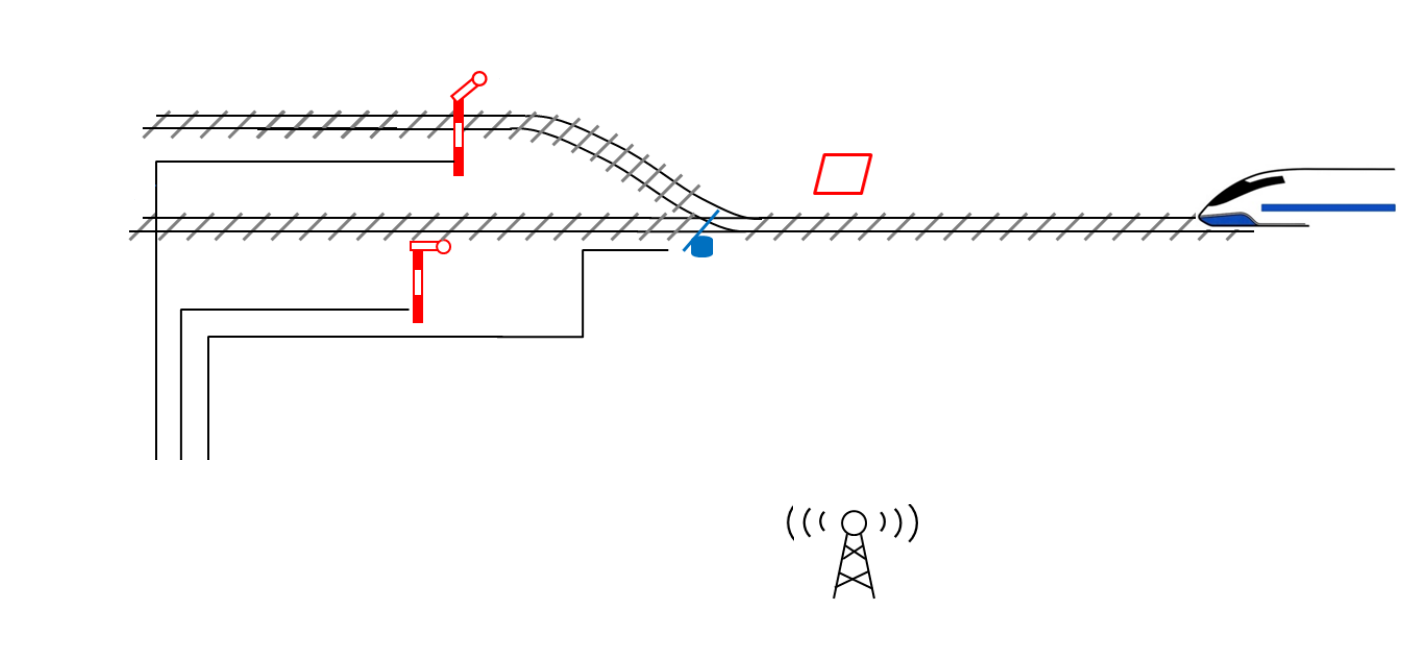
\includegraphics[width=350.8pt,height=176.4pt]{figure/railwayNetwork.png}};
%Rounded Rect [id:dp8635061097341326] 
\draw   (104.33,199.93) .. controls (104.33,192.79) and (110.12,187) .. (117.27,187) -- (156.07,187) .. controls (163.21,187) and (169,192.79) .. (169,199.93) -- (169,245.4) .. controls (169,252.54) and (163.21,258.33) .. (156.07,258.33) -- (117.27,258.33) .. controls (110.12,258.33) and (104.33,252.54) .. (104.33,245.4) -- cycle ;
%Right Arrow [id:dp5902707358380477] 
\draw   (169,199.93) -- (225.4,199.93) -- (225.4,191.7) -- (263,208.17) -- (225.4,224.63) -- (225.4,216.4) -- (169,216.4) -- cycle ;
%Rounded Rect [id:dp6848372643216789] 
\draw   (261.67,195.93) .. controls (261.67,188.79) and (267.46,183) .. (274.6,183) -- (313.4,183) .. controls (320.54,183) and (326.33,188.79) .. (326.33,195.93) -- (326.33,241.4) .. controls (326.33,248.54) and (320.54,254.33) .. (313.4,254.33) -- (274.6,254.33) .. controls (267.46,254.33) and (261.67,248.54) .. (261.67,241.4) -- cycle ;
%Right Arrow [id:dp00995349944529833] 
\draw   (261.74,249.63) -- (205.34,250.14) -- (205.42,258.37) -- (167.67,242.24) -- (205.12,225.44) -- (205.2,233.67) -- (261.59,233.17) -- cycle ;
%Right Arrow [id:dp13455094966677605] 
\draw   (369.29,188.62) -- (418.51,139.44) -- (412.87,133.8) -- (456.96,112.29) -- (435.42,156.36) -- (429.78,150.72) -- (380.57,199.9) -- cycle ;
%Right Arrow [id:dp26740738968744493] 
\draw   (488.46,128.23) -- (428.65,190.74) -- (434.41,196.25) -- (383.01,226.89) -- (411.36,174.2) -- (417.12,179.71) -- (476.94,117.21) -- cycle ;

% Text Node
\draw    (238.6,28.4) -- (277.6,28.4) -- (277.6,49.4) -- (238.6,49.4) -- cycle  ;
\draw (239.6,29.4) node [anchor=north west][inner sep=0.75pt]  [font=\footnotesize] [align=left] {signal};
% Text Node
\draw    (364.6,37.73) -- (404.6,37.73) -- (404.6,75.73) -- (364.6,75.73) -- cycle  ;
\draw (365.6,38.73) node [anchor=north west][inner sep=0.75pt]  [font=\footnotesize] [align=left] {virtual\\signal};
% Text Node
\draw    (311.93,111.07) -- (352.93,111.07) -- (352.93,132.07) -- (311.93,132.07) -- cycle  ;
\draw (312.93,112.07) node [anchor=north west][inner sep=0.75pt]  [font=\footnotesize] [align=left] {switch};
% Text Node
\draw    (123.27,32.4) -- (192.27,32.4) -- (192.27,53.4) -- (123.27,53.4) -- cycle  ;
\draw (124.27,33.4) node [anchor=north west][inner sep=0.75pt]  [font=\footnotesize] [align=left] {track circuit};
% Text Node
\draw    (149.27,147.73) -- (192.27,147.73) -- (192.27,168.73) -- (149.27,168.73) -- cycle  ;
\draw (150.27,148.73) node [anchor=north west][inner sep=0.75pt]  [font=\footnotesize] [align=left] {cables};
% Text Node
\draw (115.33,211.33) node [anchor=north west][inner sep=0.75pt]   [align=left] {IS};
% Text Node
\draw (274.67,209.33) node [anchor=north west][inner sep=0.75pt]   [align=left] {RBC};
% Text Node
\draw (169,199.93) node [anchor=north west][inner sep=0.75pt]  [font=\footnotesize] [align=left] {element states};
% Text Node
\draw (190.67,232) node [anchor=north west][inner sep=0.75pt]  [font=\footnotesize] [align=left] {train data};
% Text Node
\draw (365.02,188.71) node [anchor=north west][inner sep=0.75pt]  [font=\footnotesize,rotate=-315.58] [align=left] {movement authority\\};
% Text Node
\draw (387.02,206.04) node [anchor=north west][inner sep=0.75pt]  [font=\footnotesize,rotate=-315.58] [align=left] {position, track requests\\};


\end{tikzpicture}


}
%\caption{Railway network.}
%\label{fig:railwayNetwork}
%\end{figure}
%%

\begin{comment}
	To better understand the structure and complexity of the railway network, Figure \ref{fig:railwayNetwork} illustrates the various components and their interconnections. As the latter demonstrates, the \gls{is} is the core of the entire system, with all the railway elements and the \gls{rbc} connected to it. This allows for centralized control and real-time monitoring of the entire network, ensuring the safe and efficient operation of the railway system.
\end{comment}


The current communication technology present on the railway infrastructure is \gls{v2i}, namely, the communication between the \gls{rbc} and trains. The existing standard \gls{v2i} is an integral component of the railway communication infrastructure, relying on the GSM-R network. Nowadays, the emergence of the 5G network-based railway communication technology, known as Future Railway Communication and Management System\cite{frmcs}, is a viable \gls{v2v} technology. It is, indeed,  gradually gaining prominence due to its advanced capabilities in data transfer, reliability and  low-latency characteristics, ensuring swift and real-time data exchange among trains within the network.


The growing popularity of trains as a mode of transportation presents a challenge of overburdening the railway system's capacity. As a result, enhancing infrastructure utilization and increasing capacity are two crucial objectives that railways are currently striving to achieve. These goals are being tackled by Shift2Rail~\cite{shift2rail}, an initiative focused on developing innovative technologies and solutions to enhance the efficiency, safety, and sustainability of the railway system.



In the following, we will introduce two \gls{ertms} technology standards, upon which the work is based: \gls{l3} and \gls{vc} which are depicted in Figure~\ref{fig:ertmsl3vc}.
 \begin{figure}[h]
	\resizebox{\linewidth}{!}{


\tikzset{every picture/.style={line width=0.75pt}} %set default line width to 0.75pt        

\begin{tikzpicture}[x=0.75pt,y=0.75pt,yscale=-1,xscale=1]
%uncomment if require: \path (0,300); %set diagram left start at 0, and has height of 300

%Image [id:dp9645385719858803] 
\draw (328.5,141.07) node  {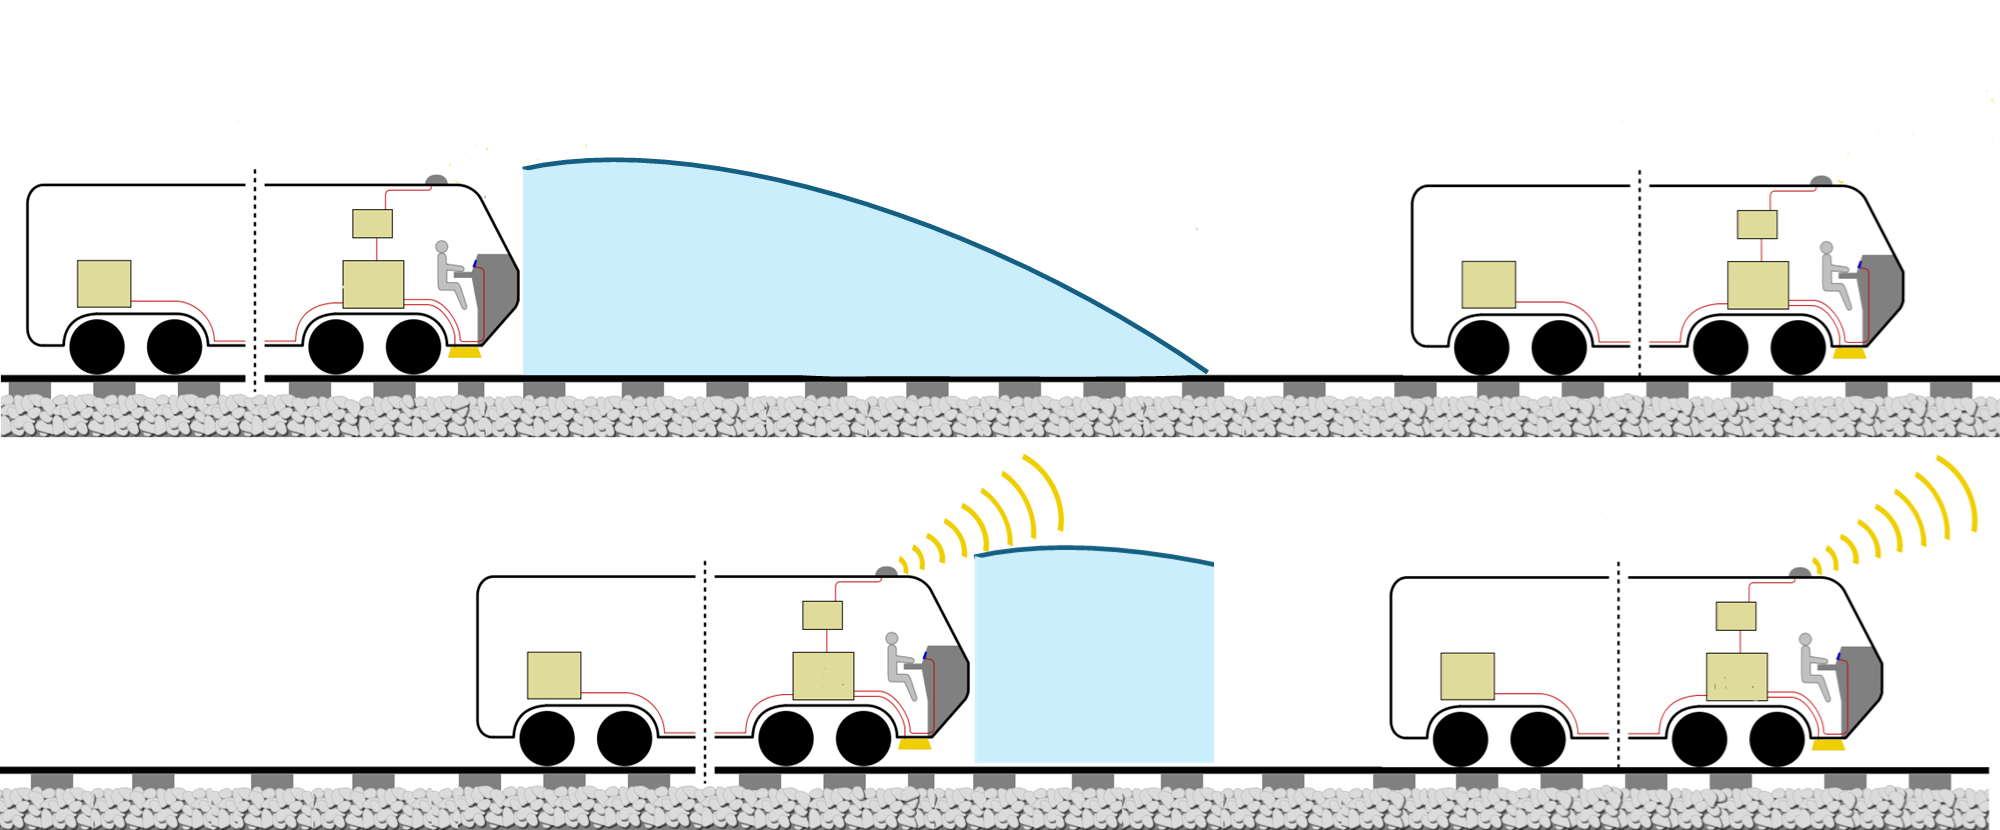
\includegraphics[width=623.25pt,height=272.36pt]{figure/Part3/levels.png}};



% Text Node
\draw (-6.27,5.95) node   [draw, fill= lightgray, line width=0.75 mm, align=left] 
{\Huge {\fontfamily{ptm}\selectfont L3}};

% Text Node
\draw (-4.67,196.95) node   [draw, fill = lightgray, line width=0.75 mm, align=left] 
{\Huge {\fontfamily{ptm}\selectfont VC}};





,\end{tikzpicture}
}
	\caption{Comparison scenarios between \gls{l3} and \gls{vc}.
		The blue area beneath the curve represents the absolute braking distance required to stop the train.}
	\label{fig:ertmsl3vc}
\end{figure} 

 By transitioning from fixed to virtual block systems, \gls{l3} reduces dependence on trackside signals and infrastructure, relying instead on advanced onboard systems and continuous  communication. This shift not only enhances line capacity but also reduces operational costs by optimizing train headways and minimizing the need for trackside maintenance; furthermore, it allows trains to move dynamically within a virtual continuously updated block which  is contingent upon the position of the preceding train~\cite{ertmsl3}.  
 



Nowadays, the technology for \gls{vc} is still in the conception stage, and research is underway to determine the best way to implement it~\cite{flamini2018}. The control field is particularly interested in finding a solution that can provide the necessary velocity, reliability, and safety to support real-time communication between trains. In addition to these technical considerations, research in the control field is also underway to determine the best way to implement \gls{vc} from an operational perspective~\cite{dimeo2020}. This involves studying the impact of the new technology on train operations and identifying the best practices for integrating the technology into the existing railway network~\cite{ertmsl4}.


 In conclusion, \gls{vc} presents a notable advantage in reducing railway delays, particularly in departure times. This innovative system holds the potential to decrease departure delays by optimizing train coordination and spacing. Promoting a more synchronized and efficient operation, \gls{vc} emerges as a valuable solution to increase the capacity and enhance punctuality across the railway network.
%
\subsection{Related Works}
\label{subsec:relatedWorks}

 A fair amount of work exists on the topic of \gls{vc} and in particular regarding the control techniques developed~\cite{wu2023railway}. The main technologies mentioned include: consensus-based control~\cite{wu2023dynamics}, constraint following control~\cite{zhang2023optimal,wang2022constraint}, sliding mode control~\cite{park2022,liu2023method}, \gls{mpc}, and \gls{ml}-based control. Emphasis will be given to the last two types, as they prove to be the most promising in this field; specifically, the latter is the type upon which the control system presented in this paper is based.

The integration of \gls{ml} into control algorithms has gained significant attention in the context of railway systems, particularly concerning virtual coupling~\cite{basile2022roadmap}. In~\cite{wang2021}, the use of \gls{rl} is proposed to obtain an optimal policy for IoT-based \gls{vcts}. The proposed approach combines \gls{rl} and artificial potential field to achieve global optimal policy and increase efficiency. Simulation results demonstrate the effectiveness of the proposed \gls{rl}-based cooperative control approach for IoT-based \gls{vcts}. The control strategy presented in~\cite{BASILE2024108120} shows a decentralized \gls{vc} using a \gls{rl} approach based on the \gls{ddpg} algorithm, with a focus on robustness and safety. The robustness is evaluated solely through Monte Carlo simulations, considering parameter uncertainties of the dynamical system. However, the approach does not provide formal analytical guarantees of robustness or safety. Additionally, the strategy does not account for communication impairments from communication channel, including time-varying delays in \gls{v2v} communication, packet losses, or switching topologies. While Monte Carlo simulations provide empirical insights, formal guarantees remain absent for these challenging scenarios.
%
The bottleneck of this \gls{ml}-based control type lies in the foundations of its theory. Currently, in the railway domain, it is not yet possible to certify an \gls{ml}-based controller according to railway safety standards, therefore making such approaches not realisic.

The approaches most closely related to our solution are the works in~\cite{felez2019model} and~\cite{wu2021virtually}. In~\cite{felez2019model}, a novel train control system utilizing virtual coupling is introduced. This system employs a decentralized model predictive control framework to optimize the control of both leading and following trains in a convoy. Comparative analyses, particularly against the moving block system, reveal improved performance, demonstrating the virtual coupling's efficacy in reducing headway and ensuring safe train separation. A linear \gls{mpc} optimizing goals like track spacing, velocity, and comfort is implemented in~\cite{wu2021virtually}. Constraints, including line velocity, collision avoidance, and traction/braking, are considered. In this work, although  safety constraints are considered inside the controller, no certification of safety is demonstrated. Compared with these two contributions, our control scheme takes into account the intrinsic characteristics of the communication channel and assumes a heterogeneous platoon with parameters uncertainty. In both~\cite{felez2019model} and~\cite{wu2021virtually}, the authors propose decentralized linear \glspl{mpc} to realize the \gls{vc} and assume the two trains can communicate in a reliable sampled framework.
In our framework we also consider (nonlinear) \glspl{mpc} but we do not focus on this aspect in details. 
Rather, in this paper we propose a hybrid/switching control architecture able to robustly satisfy safety constraints and reducing unnecessary follower train brakings, also considering not reliable communication between trains. Our framework is able to cope with diverse (\gls{mpc} based) controller choices, both for the leader and the follower. 

Details on our contribution are provided next.


 %
\subsection{Contribution}
\label{subsec:contribution}
%

In this article, we introduce a control system architecture
allowing the transition from \gls{l3} to \gls{vc} and manage \gls{vc} operations. 

Specifically, the VC is a condition under which two trains are spaced not less than a safety distance $d$ and, in principle, try to be spaced as close as possible to $d$. 
However, in the solution we propose the distance between the two trains may vary during the trains journey according to the operating conditions (but always keeping the prescribed minimum safety distance $d$).



The contributions of our work is articulated through the following key points:

\begin{enumerate}
	
 \item Our architecture addresses the twofold challenge of parameter uncertainty within train system models and the throughput variability in data packet communication channel characteristics. We establish a robust control system framework that is specifically engineered to accommodate these variabilities, always ensuring safety and reliable performance.


\item For ensuring safety, we incorporate into the design of our control architecture a safety control barrier function. This allows to certify safety guarantees and  prioritize operational safety.

\item The control architecture allows to implement very general control laws (we provide a switched controller but other choices are possible), guaranteeing not only safety, but also  avoiding as much as possible follower emergency braking when no information are received from the leader.

\item To validate the applicability and safety of our control system, we have developed a specialized railway simulation tool for \gls{vc}. This tool enables testing and evaluation of the control system across various scenarios. The demonstration of the system's effectiveness in these tests not only proves its operational viability but also solidifies its foundational role in advancing railway safety.
\end{enumerate}
%
The paper is organized as follows: Section \ref{sec:proposedarchitecture} provides an initial overview of the problem and the proposed control system architecture, the principal blocks implemented are reported. Section \ref{sec:Background} introduces safe sets and control barrier functions, ensuring system safety through robust and safety-compliant controllers, which maintain the system within safe operational conditions despite uncertainties. Section \ref{sec:TrainModeling} models the train's longitudinal dynamics defining the uncertain system parameters and ensuring safety with a robustification technique.
  Section \ref{sec:SafetyGuarantee} introduces braking and emergency controller definitions, used to ensure robust safety compliance for the train system.
  Section \ref{sec:controlsystem} provides a detailed description of the control system architecture for trains operating under \gls{vc}. It thoroughly examines the primary components and their interactions, offering insights into the design and functionality of each block within the system. This section highlights the innovative approaches used to manage the complexities of VC, ensuring efficient and safe train operations. Section \ref{sec:Simulations} presents the different operational scenario simulations
  and results. Finally, Section \ref{sec:conclusion} includes the conclusions and future works.
  
   
	
	





%%% END SECTION ============================================================
%%% START SECTION ==========================================================
\section{Addressed problem and proposed control architecture}
 \label{sec:proposedarchitecture}

In this section we provide a preliminary description of the problem addressed in the paper and the proposed control architecture. 
Specifically, we consider asynchronous communication between the leader and the follower over an unreliable communication channel. 
Leader sends packets about its planned trajectory (more precisely it will be a robust information about the planned trajectory). Such packets might be received with delay (or not received at all) by the follower. 

The problem to be addressed is the one of controlling the trains according to a ``virtual coupling'' (\gls{vc}) scheme. Specifically, the follower train should move in a coordinated way with the leader, keeping a safety distance of at least $d$ (which is a provided control parameter). The aim of the \gls{vc} is to reduce the spacing between the trains on the railway and so increase its capacity. 
Often, when referring to \gls{vc} in the literature, the distance between the trains is imposed to be exactly $d$. 

In our control architecture, instead, the inter-trains distance might vary (but never being below $d$) according to the operating condition. Implicitly, the control architecture will  control the inter-train distance guaranteeing safety and avoiding unnecessary train braking. 
This will be achieved through several control blocks simultaneously working. All these blocks run on the follower side. 

Specifically:
\begin{itemize}
\item The {\em Leader robust lower proxy (RLP) predictor block} is responsible of predicting the evolution of a system (namely the RLP) that provides a lower bound of the true leader trajectory subjected to an hypothetical emergency braking (that is, the maximum allowed deceleration). 
This block will be reset at follower packets receptions with the updated state of the leader. 
\item The {\em Safety control block} is fed with the output of the leader RLP predictor and the actual state of the follower. It continuously monitor for the overall system safety via a suitable control barrier function. Such monitoring runs on predicted information even if no updates are received from the leader. If conditions are detected such that safety might be a risk, an emergency braking is imposed to the follower, overlapping any other possible control. The emergency braking is kept until safety conditions are restored (including new leader updates). The safety control block guarantees safety in a certified manner and robustly with respect to follower and leader parameters uncertainties and communication network unreliability. 
\item The {\em Cruise virtual coupling control block} manages the follower during the normal cruise (i.e., when no safety issues are raised). It implements a predictive controller over a receding horizon while keeping the position of the follower at a certain (time-varying) distance from the leader. This distance is such that, if no updates are received, the follower can still move with its planned velocity for a given tunable amount of time before possibly trigger an emergency braking. 
This feature allows to implicitly regulate the inter-train distance according to the characteristics of the communication channel, enlarging or squeezing this dwell time in presence of less or more reliable communication (respectively). 

\item The {\em  Delay estimator block} continuously calculates the communication delay between the leader and follower by analyzing packet arrival times. This real-time estimation allows the control system to adjust reference trajectories based on current delay conditions, ensuring smooth coordination despite channel variability. The block interacts with the Cruise virtual coupling block to maintain system safety and minimize the impact of communication delays on overall performance.
\end{itemize} 
It is worth mentioning that the proposed architecture does not prescribe a specific controller. Rather, it provides an environment enabling several possible controller choices, leaving the specific design to the developer. 
Therefore, while in this paper we propose a switching controller over three possible operational modes (with more or less aggressive maneuvers according to the inter-train distance), several other choices are possible. 
Also, our framework seamless allows the implementation of any additional safety criteria or the integration of other modules/features, such as the online estimation of the channel quality and characteristic delay, so as to adjust in real-time the dwell time in the Cruise virtual coupling control block. Such block is presented in this paper but not strictly necessary for safety and stability. 






%%% END SECTION ============================================================
%%% START SECTION ==========================================================
\section{Background}
 \label{sec:Background}
 





\subsection{Dynamical system and Barrier Function}
\label{subsec:barrier}

Here we introduce the concept of safe set and barrier function. We keep our illustration rather informal and we only provide those concepts which will be useful in the rest of the paper. For this reason we do not always follow a ``standard" notation and cast this background for the specific problem in hand.  Further details can be found in several papers and books in the literature, see for example \cite{belta} and references therein. 


Let us consider a dynamical system described by 
\begin{subequations}\label{eq:dynamical_system}
\begin{align}
	& \dot{x}(t) = f(x(t), u(t)), \label{eq:dynamics}\\
	& \mathcal{C}(x(t),u(t))\leq 0 \label{eq:constraints}\\
	& x_0=x(t_0). \label{eq:initial_condition}
\end{align}
\end{subequations}
where $t \in \mathbb{R}_+
$ is the time, \(x \in \mathbb{R}^n\) is the state of the system, \(u \in \mathbb{R}^m\) the control input, $f: \Bbb{R}^n \times\Bbb{R}^m \rightarrow \Bbb{R}^n $ the (smooth) dynamical function and $\mathcal{C}: \Bbb{R}^n \times\Bbb{R}^m \rightarrow \Bbb{R}^l$ provides static constraints. 





Let us consider a {\em safe set} $\mathcal{S}\subseteq \Bbb{R}^n$, that is a set of the state space where we aim to confine the state of the system. 


\begin{definitionNoPoint}[CBF]
Let us consider a dynamical system \eqref{eq:dynamical_system} and a safe set $\mathcal{S}\subseteq \Bbb{R}^n$. 
A {\em control barrier function on $\mathcal{S}$} is any continuous function $b(x): \Bbb{R}^n \rightarrow \Bbb{R}$ such that 
\begin{equation}\label{eq:barrier_function}
b(x) \leq 0 \iff x \in \mathcal{S}.\\
\end{equation}
\end{definitionNoPoint}



Notice that some authors in the literature reverse the sign of the inequality in the above definition; this, obviously, is only a convention that does not alter its meaning. Also, in the literature a further hypothesis on $b(x)$ is being continuously differentiable. In our paper we do not ask for this requirement and we will consider $b(x)$ continuous only. 




Control barrier function are particularly useful in control theory when there is the need of certifying system safety. Specifically, we give the following definition. 

\begin{definitionNoPoint}
Let us consider a dynamical system \eqref{eq:dynamical_system}
and an initial condition $x_0$ such that $b(x_0)\leq 0$ and a control input $u(t)$, with $t\in [t_0, +\infty)$. 

The trajectory $x(t)=\phi(t,t_0,x_0,u)$ is said to be {\em safe} if $b(x(t))\leq 0$ for all $t\in [t_0, +\infty)$. If $x(t)$ is safe, $u(t)$ is said a {\em safe control trajectory}.

\end{definitionNoPoint}


\begin{definitionNoPoint}
Let us consider a feedback controller \( u = K(x) \) for system\tildeAdd\eqref{eq:dynamical_system} and, with some abuse of notation, let \(\phi(t, t_0; x_0, K(\cdot))\) denote the closed-loop state \( x(t) \). It is said a {\em safe} controller for set $\mathcal{S}$ if for any $x_0$ such that $b(x_0)\leq 0$, the trajectory  $x(t)=\phi(t,t_0,x_0,K(\cdot))$ is safe.
\end{definitionNoPoint}

Roughly speaking, the above definition means that $K(\cdot)$ is safe if, for any safe initial condition, it keeps the system in the safe set forward in time. 

A further (stronger) definition for a feedback controller is provided in what follows.


\begin{definitionNoPoint}\label{def:safety_compliant}
Let us consider a feedback controller $u=K(x)$ for system  \eqref{eq:dynamical_system} and let $x(t)=\phi(t,t_0,x_0,K(\cdot))$ be the system solution. 
The controller is said {\em safety compliant} for set $\mathcal{S}$ if
\begin{itemize}
\item [i.]  $K(\cdot)$ is safe;
\item [ii.] for any $x_0$ such that $b(x_0)>0 $, the function $b(x(t))$ with $t\in [t_0, \bar{t}]$ is monotonically decreasing (not necessarily strictly) for any $\bar{t}$ such that $b(x(\bar{t}))>0$. 
\end{itemize}

\end{definitionNoPoint}

Roughly speaking, the above definition qualifies any controller able to keep safety when the system starts in the safe set and able not to ``increase'' the unsafety (that is, the value of $b(x(\cdot))$ for any unsafe initial condition. 



With respect to Definition\tildeAdd\ref{def:safety_compliant}, let us call $\mathcal{T}\subseteq [t_0, +\infty) $ the set of the time instants where $b(x(t))$ is strictly monotone, that is $b(x(t_1))>b(x(t_2))$ for any $t_1,t_2\in \mathcal{T}$ with $t_1<t_2$.
The following result holds.

\begin{theorem} \label{thm:safety-compliant}
Let us consider a smooth dynamical system  \eqref{eq:dynamical_system}, a smooth feedback controller $K(x)$ and a continuous control barrier function $b(x)$ defined for the safe set $\mathcal{S}$. 
Suppose that the controller is safety compliant and the trajectory
$x(t)=\phi(t,t_0,x_0,K(\cdot))$ is bounded for any valid initial condition $x_0\in\Bbb{R}^n$ (that is, satisfying constraints \eqref{eq:constraints}). Also, suppose  $\mathcal{T}$ unbounded.
Then, the limit set  $\omega(x_0)\subseteq \mathcal{S}$ for all $x_0$, \cite{khalil}.

\end{theorem}

 
 
  \begin{proof}
We need to prove the results only for those $x_0\notin \mathcal{S}$, since for $x_0\in\mathcal{S}$ the result trivially comes from Definition\tildeAdd\ref{def:safety_compliant}.
First of all, consider a sequence of time instants $t_k\in \mathcal{T}$,  with $\lim_{k\rightarrow +\infty} t_k=+\infty$ (this can be done since $\mathcal{T}$ is supposed to be unbounded).
The proof will be conducted with a contradiction argument.
Let us suppose $\lim_{k \rightarrow +\infty} b(x(t_k))=\bar{b}$, with $\bar{b}>0$. Let us call $b^{-1}(	\bar{b}):\{x\in\Bbb{R}^n: b(x)=\bar{b}\}$. 
We obviously have $b^{-1} (\bar{b})\cap \mathcal{S}=\emptyset$. Let us consider the limit set $\omega(x_0)$ (note that such set is not empty since $x(t)$ is bounded, see \cite{khalil}). We trivially have $\omega(x_0)\subseteq b^{-1} (\bar{b})$.

Let us consider a point $\tilde{x}\in\omega(x_0)$, a finite time span $\tau >0$ and an index sequence $h$ such that $t<t_h\leq t+\tau$. By the smoothness of $f(\cdot)$ and $K(\cdot)$, the function $\phi(t+\tau, t, \tilde{x}, K(\cdot))$ is continuous with respect to the variable $\tilde{x}$ for any initial time $t$ {and evolution} length $\tau$.
Calling $\tilde{b}=b(\phi(t+\tau, t, \tilde{x}, K(\cdot)))$, we have $\tilde{b}<\bar{b}$.
Let us choose a $\varepsilon<\bar{b}-\tilde{b}$. Then, by continuity we have that there exists a $\delta >0$ such that any $\hat{x}$ such that $\|\tilde{x}-\hat{x}\|<\delta$ implies 
\begin{equation*}
\|b(\phi(t+\tau, t, \tilde{x}, K(\cdot)))-b(\phi(t+\tau, t, \hat{x}, K(\cdot)))\|<\varepsilon.
\end{equation*}

A direct consequence of the above inequality is that 
$b(\phi(t+\tau, t, \hat{x}, K(\cdot))<\tilde{b}$ which implies that $\tilde{x}$ cannot belong to $\omega(x_0)$. Since this reasoning can be conducted for any point in $\omega(x_0)$, we have that the latter set is empty, leading to a contradiction. The reasoning can be repeated for any $\tilde{b}>0$ implying that $\omega(x_0)\in\mathcal{S}$.
 
\end{proof}








Let us now consider a variation of system \eqref{eq:dynamical_system}, namely 
\begin{subequations}\label{eq:dynamical_system_param}
\begin{align}
	& \dot{x}(t) = f(x(t), u(t),p),\\
	& \mathcal{C}(x(t),u(t),p)\leq 0,\\
	& x_0=x(t_0), \\
	& u = K(x),
\end{align}
\end{subequations}
where we explicitly pointed out the dependency of the system on a parameter vector $p\in \mathcal{P}\subset \Bbb{R}^q$, with $\mathcal{P}$ bounded set. 

Obviously, system \eqref{eq:dynamical_system_param} solution depends on the value of $p$, that is  $x(t)=\phi(t,t_0,x_0,K(\cdot),p)$.
It could be the case (as in our manuscript) that the value of parameter $p$ is not know. For this reason,
we provide the following definitions. 

\begin{definitionNoPoint}
Let us consider a feedback controller $u=K(x)$ for system  \eqref{eq:dynamical_system_param}.
The controller is said {\em robustly safe} if, for any $x_0$ such that $b(x_0)\leq 0$, the trajectory  $x(t)=\phi(t,t_0,x_0,K(\cdot),p)$ is safe for any $p\in \mathcal{P}$.
\end{definitionNoPoint}


\begin{definitionNoPoint}
Let us consider a feedback controller $u=K(x)$ for system  \eqref{eq:dynamical_system_param}.
The controller is said {\em robustly safety compliant} if it is safety compliant for any $p\in \mathcal{P}$.
\end{definitionNoPoint}


The following theorem holds.

\begin{theorem} \label{lemma:safety-enforcing-robust}
Let us consider the dynamical system  \eqref{eq:dynamical_system_param} smooth for any $p\in\mathcal{P}$, a smooth feedback controller $K(\cdot)$ and a continuous control barrier function $b(\cdot)$ defined for the safe set $\mathcal{S}$. 
Suppose that the controller is robustly safety compliant and the trajectory
$x(t)=\phi(t,t_0,x_0,K(\cdot),p)$ is bounded for any $p\in\mathcal{P}$ and any valid initial condition $x_0\in\Bbb{R}^n$. Then, the limit set $\omega(x_0,p)\subseteq \mathcal{S}$ for all $x_0$.

\begin{proof}
The proof is a direct consequence of Theorem \ref{thm:safety-compliant} applied at any dynamical system model for any parameter value $p$.
\end{proof}
\end{theorem}


Finally, we provide the following definition. 

\begin{definitionNoPoint}\label{def:protecting_barrier}
Let us consider a (possibly parameter dependent) dynamical system in the general form \eqref{eq:dynamical_system_param} and suppose $\mathcal{S}^\prime\subseteq \Bbb{R}^n$ is its safe set. Suppose also to consider another set $\mathcal{S}$ such that $\mathcal{S}\subseteq \mathcal{S}^\prime$ and a CBF $b(x)$ on $\mathcal{S}$ (that is, considering $\mathcal{S}$ as safe set). We will say that $b(x)$ {\em protects} $\mathcal{S}^\prime$.
\end{definitionNoPoint}

\begin{lemma}\label{lem:protecting_barrier}
Let us consider a dynamical system  \eqref{eq:dynamical_system_param} and sets $\mathcal{S}\subseteq\mathcal{S}^\prime\subseteq \Bbb{R}^n$, with $\mathcal{S}^\prime$ safe set for the system. Consider a CBF $b(x)$ protecting $\mathcal{S}^\prime$ and a feedback controller $u=K(x)$. The following points hold:
\begin{itemize}
\item [i.] If $K(\cdot)$ is a safe controller for $\mathcal{S}$, it is also a safe controller for $\mathcal{S}^\prime$;
\item [ii.] If $K(\cdot)$ is a safety compliant controller for $\mathcal{S}$, it is also a safety compliant controller for $\mathcal{S}^\prime$.
\end{itemize}

\begin{proof}
The proof trivially derives from the inclusion relation between set  $\mathcal{S}$ and $\mathcal{S}^\prime$.
\end{proof}
\end{lemma}




\subsection{Setting}
\label{subsec:setting}
In this paper, similarly to what done in \cite{felez2019model}, we consider two consecutive trains on the same line, the leader (denoted with superscript $\mathrm{L}$) and the follower (denoted with superscript $\mathrm{F}$) (the extension to more than two trains is not addressed in the paper, although the proposed framework allows for that, which is left as a future work).

Both leader and follower have a dynamical model (whose details are provided later) summarized as 
\begin{subequations}\label{eq:dynamical_system_param_i}
\begin{align}
	& \dot{x}^i(t) = f^i(x^i(t), u^i(t),p^i), \label{eq:dynamical_system_param_i_dynamics}\\
	& \mathcal{C}^i(x^i(t),u^i(t),p^i)\leq 0, \label{eq:dynamical_system_param_i_constraints}\\
	& x_0^i=x^i(t_0), \label{eq:dynamical_system_param_i_initial}
\end{align}
\end{subequations}
with $x^i\in \Bbb{R}^{n_i}$, $u^i\in \Bbb{R}^{m_i}$,  $p^i\in \mathcal{P}^i\subset \Bbb{R}^{q_i}$, $\mathcal{C}^i(\cdot)\in \Bbb{R}^{l_i}$, with $i\in\{\mathrm{L}, \mathrm{F}\}$. 

The controllers of the two trains have generic expressions $K^\mathrm{L}$ and $K^\mathrm{F}$.


Notice that, via stacking $x=[{x^\mathrm{L}}^T, {x^\mathrm{F}}^T]^T$, $u=[{u^\mathrm{L}}^T, {u^\mathrm{F}}^T]^T$, $p=[{p^\mathrm{L}}^T, {p^\mathrm{F}}^T]^T$, $x_0=[{x_0^\mathrm{L}}^T, {x_0^\mathrm{F}}^T]^T$, $f=[{f^\mathrm{L}}^T, {f^\mathrm{F}}^T]^T$, $\mathcal{C}=[{\mathcal{C^\mathrm{L}}}^T, {\mathcal{C^\mathrm{F}}}^T]^T$ and setting $n=n_\mathrm{L}+n_\mathrm{F}$, $m=m_\mathrm{L}+m_\mathrm{F}$, $l=l_\mathrm{L}+l_\mathrm{F}$ and $q=q_\mathrm{L}+q_\mathrm{F}$ the overall dynamical system is formally represented by \eqref{eq:dynamical_system_param}, with controller $K=[{K^\mathrm{L}}^T, {K^\mathrm{F}}^T]^T$. 

Both controller $K^\mathrm{L}$ and $K^\mathrm{F}$ will be applied over a receding horizon (more details about these controllers will be provided later). The overall horizon for the leader is called $H$.



%
\subsection{Channel Communication}
\label{subsec:transmissionEvent}
 %
 %


In this study, we consider the train communication under \gls{ertms} technology, which  utilizes an event-triggered transmission protocol. This approach entails the transmission of signals or messages in response to specific operational events or conditions. We specifically consider the challenges posed by communication delays and packet losses within the \gls{v2v} context.
In this regard, here we abstract how the communication happens on the physical layer and its implementation mechanisms (either via a direct communication between leader and follower or via the railway infrastructure) and focus on all its control related aspects.


Specifically, the leader transmits its information, from the current value up to a horizon \(H\). Transmissions happen at instants \(\{ t_{\kappa^\mathrm{L}} \}_{\kappa^\mathrm{L}=0}^{+\infty}\) via sending the tuple $\left ( t_{\kappa^\mathrm{L}}, x^\mathrm{L}(t_{\kappa^\mathrm{L}}),\underline{\mathbf{x}}^\mathrm{L}(t_{\kappa^\mathrm{L}})\right)$, where $t_{\kappa^\mathrm{L}}$ is the trigger instant, $x^\mathrm{L}(t_{\kappa^\mathrm{L}})$ the state of the leader and 
$\underline{\mathbf{x}}^\mathrm{L}(t_{\kappa^\mathrm{L}})=\underline{x}^\mathrm{L}(t)_{t\in [t_{\kappa^\mathrm{L}}, t_{\kappa^\mathrm{L}} + H]}$ the whole robustly predicted state of the leader (due to its own control trajectory) up to horizon $H$.
More details on  such robust state estimation trajectory and in which sense it can be considered robust will be provided later. 

The leader transmission instants \(\{ t_{\kappa^\mathrm{L}} \}_{\kappa^\mathrm{L}=0}^{+\infty}\) might be generated periodically or asynchronously (due to some event-triggered logic of the leader controller). In the current ERTMS, transmissions happen synchronously on a fixed period base. Therefore, for validating our algorithm we used in Section \ref{sec:Simulations} 
a fixed sampling time transmission. However, the whole framework we are going to develop can perfectly work with non periodic transmissions. 

The follower receives the leader data packets at instants  \(\{ t_{\kappa^\mathrm{LF}} \}_{\kappa^\mathrm{LF}=0}^{+\infty}\).

Notice that, due to packet losses and delays  in the communication or stochastic processing time, leader packets are not received synchronously by the follower (or not received at all), in other words
	\[\{ t_{\kappa^\mathrm{L}} \}_{\kappa^\mathrm{L}=0}^{+\infty} \neq \{ t_{\kappa^\mathrm{LF}} \}_{\kappa^\mathrm{LF}=0}^{+\infty}.\]
	


The following functions are defined to represent the last trigger time for the leader and follower, respectively, enabling a precise analysis of data transmission timing:
\begin{align*}
	\ell_{\kappa^\mathrm{L}}(t) &= \max_{t_{\kappa^\mathrm{L}} \leq t} \left \{ t_{\kappa^\mathrm{L}} \right \}_{\kappa^\mathrm{L}=0}^{+\infty}, \\
	\ell_{\kappa^\mathrm{LF}}(t) &= \max_{t_{\kappa^\mathrm{LF}} \leq t} \left \{ t_{\kappa^\mathrm{LF}} \right \}_{\kappa^\mathrm{LF}=0}^{+\infty}.
\end{align*}


Suppose the leader transmits a packet at time $t_{\kappa^\mathrm{L}}$, and let $\tau(t_{\kappa^\mathrm{L}})\in \Bbb{R}^+ \cup \{+\infty\}$ denote the elapsed time of follower reception of such packet, that is the follower receives the packet at $t_{\kappa^\mathrm{L}} + \tau(t_{\kappa^\mathrm{L}})$. 


The sequence of $ \left\{ \tau(t_{\kappa^\mathrm{L}})\right\}_{\kappa^\mathrm{L}=0}^{+\infty}$ can be modeled as a random process as will be proposed in Section \ref{sec:Simulations}. Nevertheless, as it will be clearer later in the manuscript, our framework does not need a specific transmission packets delay model.











 \section{Train Modeling}
 \label{sec:TrainModeling}

The model employed in this manuscript relies on the principles of longitudinal train dynamics. It treats the train as a singular point mass with one degree of freedom. Additionally, it incorporates aspects such as the propulsion and braking system, the effects of rolling and bearing resistances, air input, the influence of aerodynamic drag, as well as the consideration of grade and curving resistances~\cite{ltdModel}:
%
  \begin{align}  \label{eq:stateDynamic}
 \dot{x}_1^i (t) &= x_2^i(t),  \nonumber \\
  \dot{x}_2^i(t) &= \frac{1}{M^i}(-A^i-B^i x_2^i(t) -  C^i (x_2^i(t))^2)-\mathrm{F}_e^i(t) + \frac{u^i(t)}{M^i}.
\end{align}
%

We utilize the symbols ${x}_1^i(t)$ and ${x}_2^i(t)$ to represent the $i$-th train's position and velocity, respectively, with $i\in\{L, F\}$. By convention, we consider a reference frame at the head of each train (therefore the position is referred to as the train head). 
Also, we consider positive positions, with the origin at the beginning of the railway. Implicitly, both position and velocity will only be nonnegative (the trains cannot move backward during normal operations). The constraints ${x}_1^i(t)\geq 0$ and ${x}_2^i(t)\geq 0$ will be therefore implicitly included in compact term \eqref{eq:dynamical_system_param_i_constraints}.
 
The state vector is compactly written as {$x^i(t)=(x_1^i(t),x_2^i(t))^T$}.
The variable $u^i(t)$ is the control driving or braking force; $\mathrm{F}_e^i$ denotes the external force originating from the track; $M^i$ denotes the mass parameter, while $A^i$ encompasses both rolling resistance and bearing resistance; $B^i$ is a coefficient related to the flange friction, and $C^i$ represents the aerodynamic coefficient.
%
In this model, $\mathrm{F}^i_e(t)$ is the $i$-th external force
%
\begin{equation*}
\mathrm{F}_e^i(t) = g \sigma(x_1^i(t)) + \frac{\gamma}{\rho(x_1^i(t))}, 
\end{equation*}
%
where $\gamma=6\cdot10^6$ is a constant parameter. It encompasses two distinct terms: the first one is the gravity force resulting from the track's slope $\sigma(x_1^i(t))$  at point $x_1^i(t)$, with $g$ representing the gravitational acceleration; the second term designates the curving resistance, with ${\rho(x_1^i(t))}$ representing the curve's radius.

Regarding the constraints on the state and input of the model, they are presented as follows
%
\begin{subequations} \label{eq:modelConstraints}
    \begin{align}
        u^i(t) &\in \left[-M^i a_{\mathrm{br}}^i, \;M^i a_{\mathrm{dr}}^i \right], \label{eq:lim1} \\
         u^i(t) \cdot x_2^i(t)&\in \left[-P^i_{\mathrm{br}}, \;P^i_{\mathrm{dr}}\right], \label{eq:lim2} \\
       x_2^i(t) &\in \left[0, \;\min\{V^{\mathrm{max},i},V^{\mathrm{line}}(x_1^i(t))\}\right], \label{eq:lim5} \\
        x_1^i(t) &\in \mathbb{R}_{+}. \label{eq:lim4}  
    \end{align}
\end{subequations}
%

All the above parameters are nonnegative and are constructional characteristics unique to each individual train and the railway.  Specifically,  $a_{\mathrm{br}}^i $ and $a_{\mathrm{dr}}^i$ correspond to the maximum braking and acceleration admitted, $P^i_{\mathrm{br}}$ and $P^i_{\mathrm{dr}}$ represent the minimum and maximum mechanical power, and $V^{\mathrm{max},i}$ and $V^{\mathrm{line}}$ denotes the maximum attainable velocity for the train and railway velocity limit at position $x_1^i$, respectively.



\subsection{Robust Modeling}
\label{subsec:robustModeling}
%
In the context of railway control, safety is of utmost importance and must be guaranteed even with parametric uncertainties. 

In this paper, the following model parameters are supposed uncertain in a given range
%
\begin{eqnarray}\label{eq:train_intervals}
   &a_{\mathrm{br}}^i \in [\underline{a}_{\mathrm{br}}^i , \overline{a}_{\mathrm{br}}^i], \;
      a_{\mathrm{dr}}^i \in [\underline{a}_{\mathrm{dr}}^i , \overline{a}_{\mathrm{dr}}^i],  \;
   P^i_{\mathrm{br}} \in [\underline{P}_{\mathrm{br}}^i , \overline{P}_{\mathrm{br}}^i]  , \nonumber \\
   &P^i_{\mathrm{dr}} \in [\underline{P}_{\mathrm{dr}}^i , \overline{P}_{\mathrm{dr}}^i],   \;
   C^i \in [\underline{C}^i , \overline{C}^i ] , M^i \in [\underline{M}^i , \overline{M}^i], \;\nonumber \\
    & A^i \in [\underline{A}^i , \overline{A}^i] ,  \;
     B^i \in [\underline{B}^i , \overline{B}^i] .
\end{eqnarray}



Compactly, we call $\mathcal{P}^i$ the Cartesian product of the above intervals.  With such a choice, and taking into account~\eqref{eq:stateDynamic}~and~\eqref{eq:modelConstraints}, the train model can be compactly  written as \eqref{eq:dynamical_system_param_i}.






\subsection{Robust Proxies}
\label{subsec:robustProxies}
%
To derive a control architecture robust against any possible parameter choice of the two trains, 
the notions of \gls{rlp} and \gls{rup} are  introduced as simple (yet effective) robustification technique. 
%
\begin{definitionNoPoint}[\gls{rlp}]\label{def:rlp}
A \gls{rlp} for the system \eqref{eq:dynamical_system_param_i} is any dynamical system of the form
%
\begin{equation} \label{eq:rlp}
     \underline{\dot{x}}^i(t) = \underline{f}^i(\underline{x}^i(t),u^i(t)),
\end{equation}
with $\underline{x}\in \Bbb{R}^{n_i}$ and $u\in\Bbb{R}^{m_i}$ and such that its dynamical flow $\underline{\phi}^i\left(t,t_0,x_0^i,u^i\right)$ satisfies 
\begin{equation}\label{lemma:rlpProxy}
\underline{\phi}^i\left(t,t_0,x_0^i,u^i\right) \leq \phi^i\left(t,t_0,x_0^i,u^i,p^i\right), 
\end{equation}
for all $x_0\in\Bbb{R}^{n_i}$, for all $u_i \in \Bbb{R}^{m_i}$, for all $t\in [t_0, +\infty)$ and for all $p^i\in\mathcal{P}^i$ and where the inequality is meant component-wise.
\end{definitionNoPoint}

Similarly, we provide the following definition. 

\begin{definitionNoPoint}[\gls{rup}]\label{def:rup}
	
A \gls{rup} for the system \eqref{eq:dynamical_system_param_i} is any dynamical system of the form
\begin{equation} \label{eq:rup}
     \dot{\overline{x}}^i(t) = \overline{f}^i(\overline{x}^i(t),u^i(t)),
\end{equation}
with $\overline{x}\in \Bbb{R}^{n_i}$ and $u\in\Bbb{R}^{m_i}$ and such that its dynamical flow $\overline{\phi}^i\left(t,t_0,x_0^i,u^i\right)$ satisfies 
\begin{equation}\label{lemma:rupProxy}
\overline{\phi}^i\left(t,t_0,x_0^i,u^i\right) \geq \phi^i\left(t,t_0,x_0^i,u^i,p^i\right)
\end{equation}
for all $x_0\in\Bbb{R}^{n_i}$, for all $u_i \in \Bbb{R}^{m_i}$, for all $t\in [t_0, +\infty)$ and for all $p^i\in\mathcal{P}^i$  and where the inequality is meant component-wise.
\end{definitionNoPoint}




As evident from the two definitions, there might exist several proxies for  \eqref{eq:dynamical_system_param_i}. In this work, we will consider the following piece-wise smooth systems.


The following system has been chosen as \gls{rlp}:
\begin{equation}\label{eq:rlp_train}
\begin{cases}
\underline{\dot{x}}_1^i(t) =   \underline{x}_2^i(t), \qquad  \qquad \qquad \qquad \qquad \qquad  \qquad  \text{if} \; u^i(t) < 0,  \\
    \underline{\dot{x}}_2^i(t) =  \frac{1}{\underline{M}^i} \left(-\overline{A}^i - \overline{B}^i \underline{x}^i_2(t) -  \overline{C}^i \left(\underline{x}^i_2(t_0)\right)^2 \right) \\ 
    \qquad \qquad \qquad  \qquad \qquad \qquad  -\overline{F}_e^i(\underline{x}^i_1(t_0)) + \frac{u^i(t)}{\underline{M}^i}, \\ \noalign{\vskip3pt}
     \textrm{with } \overline{F}_e^i(\underline{x}^i_1(t_0)) =  g \sigma_{\sup}\left(\underline{x}^i_1(t_0)\right)+ \frac{\gamma}{\rho_{\inf}\left(\underline{x}^i_1(t_0)\right)}, \\
    \noalign{\vskip9pt}
        \underline{\dot{x}}_1^i(t) =   \underline{x}_2^i(t), \qquad \qquad \qquad  \qquad \qquad \qquad \qquad \text{if} \; u^i(t) \geq 0,  \\
    \underline{\dot{x}}_2^i(t) =  \frac{1}{\underline{M}^i} \left(-\overline{A}^i - \overline{B}^i \underline{x}^i_2(t) -  \overline{C}^i \left(\underline{x}^i_2(t)\right)^2 \right) \\ 
    \qquad \qquad \qquad  \qquad \qquad \qquad-\overline{\mathrm{F}}_e^i(\underline{x}^i_1(t_0))  + \frac{u^i(t)}{\overline{M}^i}, \\
    \sigma_{\sup}\left(\underline{x}^i_1(t_0)\right) = \underset{s \in [\underline{x}_1^i(t_0),s^{H,i}]}{\max} \sigma(s), \\
    \rho_{\inf}\left(\underline{x}^i_1(t_0)\right) = \underset{s \in [\underline{x}_1^i(t_0),s^{H,i}]}{\min} \rho(s).
\end{cases}
\end{equation}
Above, $t_0$ is a time instant upon which we consider the proxy time evolution and $s^{H,i}$ is a far enough ahead train  position. Details on $t_0$ and $s^{H,i}$ will be provided later in the paper. 


Similarly, we consider the following piece-wise system as \gls{rup}:
\begin{equation}\label{eq:rup_train}
	\begin{cases}
		\dot{\overline{x}}_1^i(t) =   \overline{x}_2^i(t), \qquad  \qquad \qquad \qquad \qquad \qquad  \qquad  \text{if} \; u^i(t) < 0,  \\
		\dot{\overline{x}}_2^i(t) =  -\frac{\underline{A}^i}{\overline{M}^i}-\underline{F}_e^i(\overline{x}^i_1(t_0)) + \frac{u^i(t)}{\overline{M}^i}, \\
		\textrm{with } \underline{F}_e^i(\overline{x}^i_1(t_0)) =  g \sigma_{\inf}\left(\overline{x}^i_1(t_0)\right)+ \frac{\gamma}{\rho_{\sup}\left(\overline{x}^i_1t_0)\right)}, \\
		\noalign{\vskip9pt}
		\dot{\overline{x}}_1^i(t) =   \overline{x}_2^i(t), \qquad \qquad \qquad  \qquad \qquad \qquad \qquad \text{if} \; u^i(t) \geq 0,  \\
		\dot{\overline{x}}_2^i(t) =  \frac{1}{\overline{M}^i} \left(-\underline{A}^i - \underline{B}^i \overline{x}^i_2(t) -  \underline{C}^i \left(\overline{x}^i_2(t)\right)^2 \right) \\
		-  \underline{\mathrm{F}}_e^i(\overline{x}^i_1(t_0))  + \frac{u^i(t)}{\underline{M}^i}, \\
		\sigma_{\inf}\left(\overline{x}^i_1(t_0)\right) = \underset{s \in [\overline{x}_1^i(t_0),s^{H,i}]}{\min} \sigma(s), \\
		\rho_{\sup}\left(\overline{x}^i_1(t_0)\right) = \underset{s \in [\overline{x}_1^i(t_0),s^{H,i}]}{\max} \rho(s),
	\end{cases}
\end{equation}
where again as before $t_0$ and $s^{H,i}$ are an initial time and a position ahead to be determined later.   


 
  
The following lemma states the validity of our choice. 
  
\begin{lemma} \label{lemma:Proxies}
Systems \eqref{eq:rlp_train} and \eqref{eq:rup_train} are valid \gls{rlp} and \gls{rup} for the train dynamics \eqref{eq:stateDynamic}\--\eqref{eq:train_intervals}. 
  \begin{proof}
The proof is immediate since it suffices to consider the 
following differential equations
\begin{align*}
	\dot{\tilde{x}}^i = \overline{f}\left(\tilde{x}^i, u^i \right) - f\left(\tilde{x}^i, u^i, p^i \right), \\
	\dot{\hat{x}}^i = f\left(\hat{x}^i, u^i \right) - \underline{f}\left(\hat{x}^i, u^i, p^i \right).
\end{align*}

Since all component terms are non-negative, this ensures the positivity of the systems.

  \end{proof}
\end{lemma}

  

  
  
 \section{Safety Guarantee}
 \label{sec:SafetyGuarantee}


\begin{comment}
	\begin{definition}[Braking Controller] \label{def:brakingController}
		Given the model present in \eqref{eq:dynamical_system_param_i} we define  $u^i(t)= K_\mathrm{B}(x^i(t))$ the braking controller as follows
		\begin{equation*}
			K_\mathrm{B}(x^i(t))=
			\begin{cases}
				\tilde{u}^i(x^i(t)) \leq 0 \qquad \mathit{if}\;  x_2^i(t) \geq 0\\
				0 \qquad\qquad\qquad \mathit{if}\;  x_2^i(t) = 0.
			\end{cases}     
		\end{equation*}
	\end{definition}
\end{comment}




One of the objectives of the train control system we propose in this paper is to ensure that the two trains maintain a safety separation distance. In other words, the goal is to guarantee that the distance between the leader and follower never falls below the predefined safety threshold $d$. Remembering that the overall state is $x=[{x^\mathrm{L}}^T,{x^\mathrm{F}}^T]^T$, this is formally modeled through the safe set
%
\begin{equation} \label{eq:distance}
\mathcal{S}^\prime(x)=\{x: x_1^\mathrm{L}- x_1^\mathrm{F} \geq  L^\mathrm{L} +d\},
\end{equation}
where $L^\mathrm{L}$ is the leader's length. 

In order to ensure that the system solution always stays in $\mathcal{S}^\prime(x)$, we consider for this paper another safe set $\mathcal{S}$ such that $\mathcal{S}\subseteq \mathcal{S}^\prime$ and a protecting CBF for $\mathcal{S}^\prime(x)$, as for Definition \ref{def:protecting_barrier}. 


To do so, let us first define $\underline{\alpha}^i \left( x_2^i\right)=\min \left\{\underline{a}^i_\mathrm{br},\frac{\underline{P}^i_\mathrm{br}}{\bar{M}^i x_2^i} \right\}$. Also, considering an $\varepsilon<1$ (the latter is a tuning parameter that can be chosen slightly less than one to reduce conservatism), let us compute a ``large" deceleration of the follower
\begin{equation*}
\underline{e}^\mathrm{L}\left(x_2^\mathrm{L}\right)=-\frac{1}{\underline{M}^\mathrm{L}}  \left(-\overline{A}^\mathrm{L}-\overline{B}^\mathrm{L} (x_2^\mathrm{L})- \overline{C}^\mathrm{L}\left(x_2^\mathrm{L}\right)^2\right)+ \overline{F}_e^\mathrm{L}(x_2^\mathrm{L})+\overline{a}^\mathrm{L}_\mathrm{br}, 
\end{equation*}

and a ``small" deceleration of the follower
\begin{equation*}
\overline{e}^\mathrm{F} (x^\mathrm{F}) = \frac{\underline{A}^\mathrm{F}}{\overline{M}^\mathrm{F}}  + \underline{F}_e^\mathrm{F}(x_1^\mathrm{F})  +\varepsilon \underline{\alpha}^\mathrm{F} (x_2^\mathrm{F}).
\end{equation*}




We define the functions

\begin{subequations}
	\begin{equation}
		\centering
		b'(x) = L^\mathrm{L} + d - (x_1^\mathrm{L} - x_1^\mathrm{F}) - \frac{1}{2}\left(\frac{{x_2^\mathrm{L}}^2}{\underline{e}^\mathrm{L}(x_2^\mathrm{L})} - \frac{{x_2^\mathrm{F}}^2}{\overline{e}^\mathrm{F}(x_2^\mathrm{F})}\right),
		\label{eq:b_prime}
	\end{equation}
	\begin{equation}
		\centering
		b''(x) = L^\mathrm{L} + d - (x_1^\mathrm{L} - x_1^\mathrm{F}),
		\label{eq:barriere_function_trains}
	\end{equation}
	\begin{equation}
		\centering
		b(x) = \max\{b'(x), b''(x)\}.
		\label{eq:b_trains}
	\end{equation}
\end{subequations}



The safe set $\mathcal{S}$ corresponds to those states resulting in $ b(x)\leq 0$, that is $\mathcal{S}=\{x: b(x)\leq 0\}$ as defined in\tildeAdd\eqref{eq:barrier_function}. The following lemma holds.

\begin{lemma}\label{lem:b_trains}
Function $b(x)$ in \eqref{eq:b_trains} is a CBF protecting the set $\mathcal{S}^\prime$ in \eqref{eq:distance}.

\begin{proof}
The set $\mathcal{S}^\prime$ corresponds to those states where $b''(x)\leq 0$. Due to \eqref{eq:b_trains}, $b(x) \leq 0 \Rightarrow b''(x)\leq 0$. 
\end{proof}

\end{lemma}


Before showing further properties of the CBF $b(x)$, we first provide some definitions. 

Let us first call $\mathcal{U}^i(x^i)$ the  { \em robust set of all the admissible control inputs at state $x^i$ } for system \eqref{eq:dynamical_system_param_i}, that is 
\begin{equation}\label{eq:admissible_inputs}
\mathcal{U}^i(x^i)=\left\{u^i\in\Bbb{R}^{m_i}: \eqref{eq:dynamical_system_param_i_constraints},  \eqref{eq:lim1},  \eqref{eq:lim2} \textrm{ are satisfied }\forall p^i \in \mathcal{P}^i\right\}.
\end{equation}

Together with the above, we call the {\em robust set of all admissible braking control input at state $x^i$} for system \eqref{eq:dynamical_system_param_i} the set
\begin{equation}\label{eq:admissible_braking_inputs}
\underline{\mathcal{U}}^i(x^i)=\left\{u^i\in\mathcal{U}^i(x^i): u^i\leq 0 \right\}.
\end{equation}

We are ready to provide the following definition.
\begin{definitionNoPoint}[Braking  Controller]
We define a {\em braking  controller} $u^i= K^i_\mathrm{B}(x^i)$ any feedback function such that
\begin{itemize}
\item $u^i \in \underline{\mathcal{U}}^i(x^i)$, \, \quad if $x_2^i >0$;
\item $u^i=0$, \qquad \quad \; if $x_2^i =0$.
\end{itemize} 
\end{definitionNoPoint}


Roughly speaking, a braking controller is any controller providing a nonpositive control input whenever the velocity is greater than zero and a null control input in case of null velocity.\footnote{The case of null control input for null velocity could, in principle, be omitted since it is implicitly deducible by the positive constraint $x_2^i\geq 0$ of the system. Nevertheless, we prefer to keep it for the sake of clarity.}

Among the braking  controllers, the emergency controller is a peculiar case, where the controller attains the highest allowed braking  action.

\begin{definitionNoPoint}[Emergency Controller]\label{def:emergency_controller}
We define  {\em the emergency controller} $u^i(t)= K^i_\mathrm{E}(x^i)$ a braking  controller with
\begin{itemize}
\item $u^i = \min \underline{\mathcal{U}}^i(x^i)$, \, \, \quad if $x_2^i >0$;
\item $u^i=0$, \qquad \qquad \quad \, \, if $x_2^i =0$.
\end{itemize} 
\end{definitionNoPoint}



We are now ready for the following result. 
\begin{theorem}\label{thm:trains_barrier}
Let us consider the trains system of form \eqref{eq:dynamical_system_param_i} with $i\in\{\mathrm{L},\mathrm{F}\}$ in their stack form \eqref{eq:dynamical_system_param}. 
Let us consider any valid (that is, outputting values satisfying the system constraints) leader controller $K^\mathrm{L}$. Let us consider that $x_2^\mathrm{F}(t_0)>0$ (the follower is not standing at the initial time $t_0$).
Then, the controller $K=[{K^\mathrm{L}}^T, {K^\mathrm{F}_E}^T]^T$ is robustly safety compliant for $\mathcal{S}$ (and therefore also for $\mathcal{S}^\prime$ according to Lemma \ref{lem:protecting_barrier}).

\begin{proof}
	see Appendix\ref{appendix:proofTheorem}.
\end{proof}
%\begin{proof}
%To prove the result, let us first consider two special choices for the leader and follower controller, namely: 
%\begin{equation*}
%\hat{K}^\mathrm{L}(x^\mathrm{L})=\begin{cases}
%\overline{a}^\mathrm{L}_{\mathrm{br}} \qquad \text{if}\; x_2^\mathrm{L}>0,\\
%0 \qquad  \text{if} \; x_2^\mathrm{L}=0,
%\end{cases}
%\end{equation*}
%\begin{equation*}
%\hat{K}^\mathrm{F}(x^\mathrm{F})=\begin{cases}
%\varepsilon \underline{\alpha}^\mathrm{F}(x_2^\mathrm{F})\qquad  \text{if} \; x_2^\mathrm{F}>0,\\
%0\qquad  \text{if} \; x_2^\mathrm{F}=0,
%\end{cases}
%\end{equation*}
%with, as said, $\varepsilon<1$ (a good choice is slightly less than one). 
%
%
%
%
%Now, let us suppose to apply from the initial time $t_0$ controller $\hat{K}^\mathrm{L}(\cdot)$  and  $\hat{K}^\mathrm{F}(\cdot)$ at the leader's RLP and at the follower's RUP, respectively (evaluated on the leader and follower states). 
%
%
%Also, let us suppose for the moment that at the considered initial time $t_0$ the leader is not stopped, that $x_2^\mathrm{L}(t_0)>0$ (this hypothesis will be removed later).
%
%Notice that the assumption $x_2^\mathrm{F}(t_0)>0$  and the technical one $x_2^\mathrm{L}(t_0)>0$ are only meant to allow these two controllers, since in case a train is stopped set $\mathcal{U}^i(x^i)=\{0\}$ is the only available controller satisfying \eqref{eq:modelConstraints}.
%
%With such a choice, it is immediate to verify that the  
%leader RLP dynamics are
%\begin{subequations}\label{eq:RLP_dynamics_K_hat}
%\begin{align}
%& \dot{\underline{x}}_1^\mathrm{L}=\underline{x}_2^\mathrm{L} \label{eq:RLP_dynamics_K_hat_dynamics}\\
%& \dot{\underline{x}}_2^\mathrm{L}=-\underline{e}^\mathrm{L}\left(x_2^\mathrm{L}(t_0)\right),\label{eq:RLP_dynamics_K_hat_constraints}\\
%& \underline{x}^\mathrm{L}(t_0)=x^\mathrm{L}(t_0), \label{eq:RLP_dynamics_K_hat_initial}
%\end{align}
%\end{subequations}
%while the follower RUP dynamics are
%\begin{subequations}\label{eq:RUP_dynamics_K_hat}
%\begin{align}
%& \dot{\overline{x}}_1^\mathrm{F}=\overline{x}_2^\mathrm{F} \label{eq:RUP_dynamics_K_hat_dynamics}\\
%& \dot{\overline{x}}_2^\mathrm{F}=-\overline{e}^\mathrm{F}\left(x^\mathrm{F}(t_0)\right),\label{eq:RUP_dynamics_K_hat_constraints}\\
%& \overline{x}^\mathrm{F}(t_0)=x^\mathrm{F}(t_0).
%\label{eq:RUP_dynamics_K_hat_initial}
%\end{align}
%\end{subequations}
%
%Let us define $t_{\mathrm{st}}^{L,p}(t_0 |\hat{K}^\mathrm{L})= \min\{t\in[t_0, +\infty): \underline{x}_2^\mathrm{L}=0\}$ the stopping time of the leader RLP subjected to controller $\hat{K}^\mathrm{L}(\cdot)$ applied from time $t_0$ and, similarly, let us define $t_{\mathrm{st}}^{F,p}(t_0 |\hat{K}^\mathrm{F})= \min\{t\in[t_0, +\infty): \overline{x}_2^\mathrm{F}=0\}$ the stopping time of the follower RUP subjected to $\hat{K}^\mathrm{F}(\cdot)$ from $t_0$. 
%
%
%From the dynamics  \eqref{eq:RLP_dynamics_K_hat} and \eqref{eq:RUP_dynamics_K_hat}, we have 
%\begin{equation}\label{eq:t_stop_L_P}
%t_{\mathrm{st}}^{L,p}(t_0 |\hat{K}^\mathrm{L}) = \frac{x_2^\mathrm{L}(t_0)}{\underline{e}^\mathrm{L}\left(x_2^\mathrm{L}(t_0)\right)} + t_0
%\end{equation}
%at position (we omit the dependencies of $t_{\mathrm{st}}^{L,p}$ for the sake of brevity)
%\begin{equation}\label{eq:leader_RLP_stop_position}
%\underline{x}_1^\mathrm{L}(t_{\mathrm{st}}^{L,p} )=x_1^\mathrm{L}(t_0)+\frac{1}{2} \frac{{x_2^\mathrm{L}(t_0)}^2}{\underline{e}^\mathrm{L}\left(x_2^\mathrm{L}(t_0)\right)},
%\end{equation}
%while the follower's \gls{rup} stops at time $t_{\mathrm{st}}^{F,p}(t_0 |\hat{K}^\mathrm{F})= \frac{x_2^\mathrm{F}(t_0)}{\overline{e}^\mathrm{F}\left(x^\mathrm{F}(t_0)\right)} + t_0$ at position (again omitting the dependencies of $t_{\mathrm{st}}^{F,p}$)
%\begin{equation}\label{eq:follower_RUP_stop_position}
%\blue{MT:\overline{x}}\underline{x}_1^\mathrm{F}(t_{\mathrm{st}}^{F,p} )=x_1^\mathrm{F}(t_0)+\frac{1}{2} \frac{{x_2^\mathrm{F}(t_0)}^2}{\overline{e}^\mathrm{F}\left(x^\mathrm{F}(t_0)\right)}.
%\end{equation}
%
%
%The position difference of the two trains proxies when they are both stopped is, therefore
%\begin{equation}\label{eq:proxy_difference}
%\begin{aligned}
%\underline{x}_1^\mathrm{L}(t_{\mathrm{st}}^{L,p} ) - \blue{MT}\overline{x}_1^{F,p}(t_{\mathrm{st}}^{F,p}  )=&
%x_1^\mathrm{L}(t_0)-x_1^\mathrm{F}(t_0)\\
%&+\frac{1}{2}
%\left(\frac{{x_2^\mathrm{L}(t_0)}^2}{\underline{e}^\mathrm{L}\left(x_2^\mathrm{L}(t_0)\right)}
%-
%\frac{{x_2^\mathrm{F}(t_0)}^2}{\overline{e}^\mathrm{F}\left(x^\mathrm{F}(t_0)\right)}
%\right).
%\end{aligned}
%\end{equation}
%
%It is worth noticing that when both the proxies are stopped, being $\mathcal{U}^\mathrm{L}(\underline{x}_1^\mathrm{L}(t_{\mathrm{st}}^{L,p} ))=\{0\}$ and $\mathcal{U}^\mathrm{F}(\overline{x}_1^\mathrm{F}(t_{\mathrm{st}}^{F,p}  ))=\{0\}$, we have that $\underline{x}_1^\mathrm{L}(t)=\underline{x}_1^\mathrm{L}(t_{\mathrm{st}}^{L,p} )$ at any $t\geq t_{\mathrm{st}}^{L,p}$ and, similarly, 
%$\overline{x}_1^\mathrm{F}(t)=\overline{x}_1^\mathrm{F}(t_{\mathrm{st}}^{F,p})$ at any time $t\geq t_{\mathrm{st}}^{F,p}$. 
%
%When comparing \eqref{eq:proxy_difference} with $b^\prime(x)$ in \eqref{eq:b_prime}, it is immediate to notice that 
%\begin{equation}\label{eq:equality_b_prime}
%b^\prime([{\underline{x}^\mathrm{L}}^T(t_0),{\overline{x}^\mathrm{F}}^T(t_0)]^T)=L^\mathrm{L}+d-\left(\underline{x}_1^\mathrm{L}(t_{\mathrm{st}}^{L,p} ) -\overline{x}_1^\mathrm{F}(t_{\mathrm{st}}^{F,p}  )\right).
%\end{equation}
%
%From the above equation we have that, when evaluated at $x=[{\underline{x}^\mathrm{L}}^T(t_0),{\overline{x}^\mathrm{F}}^T(t_0)]^T$,  $b^\prime(x)$ can be interpreted as the difference between the minimum required inter-trains distance $L^\mathrm{L}+d$ and the proxy leader-follower distance achieved when considering that, at a generic initial time instant $t_0$, the two proxies engage controllers $\hat{K}^\mathrm{L}(\cdot)$ and $\hat{K}^\mathrm{F}(\cdot)$, respectively, until they stop. 
%Notice also that, in view of this interpretation, the following equality holds\footnote{To ease the notation we will write $b^\prime(\underline{x}^\mathrm{L}(t),\overline{x}^\mathrm{F}(t))$ instead of $b^\prime([{\underline{x}^\mathrm{L}}^T(t),{\overline{x}^\mathrm{F}}^T(t)]^T)$ (and similarly mutatis mutandis for the other terms on which $b(\cdot)$ is evaluated).}
%\begin{equation}\label{eq:constantb_prime}
% b^\prime(\underline{x}^\mathrm{L}(t),\overline{x}^\mathrm{F}(t))=b^\prime(\underline{x}^\mathrm{L}(t_0),\overline{x}^\mathrm{F}(t_0)),
%\end{equation}
%at any time instant $t>t_0$ with  $\underline{x}^\mathrm{L}(t)=\underline{\phi}^\mathrm{L}(t,t_0,x^\mathrm{L}(t_0),\hat{K}^\mathrm{L}(\cdot))$ and $\overline{x}^\mathrm{F}(t)=\overline{\phi}^\mathrm{F}(t,t_0,x^\mathrm{F}(t_0),\hat{K}^\mathrm{F}(\cdot))$, that is evaluated on the dynamical flow of the two proxies subjected to the controllers $\hat{K}^\mathrm{L}(\cdot))$ and $\hat{K}^\mathrm{F}(\cdot))$.
%
%For shorting the notation, let us rewrite $\underline{x}^\mathrm{L}(t | \hat{K}^\mathrm{L})$ to denote the RLP trajectory of the leader under controller $\hat{K}^\mathrm{L}(\cdot)$ and initial condition $x^\mathrm{L}(t_0)$ and, similarly  $\overline{x}^\mathrm{F}(t | \hat{K}^\mathrm{F})$ to denote the RUP trajectory of the follower under controller $\hat{K}^\mathrm{F}(\cdot)$ and initial condition $x^\mathrm{F}(t_0)$. 
%
%
%Analogously (and still considering the initial conditions $x^\mathrm{L}(t_0)$ and $x^\mathrm{F}(t_0)$), let us denote with $x^\mathrm{L}(t | \hat{K}^\mathrm{L})$  and $x^\mathrm{F}(t | \hat{K}^\mathrm{F})$ the trajectory of the leader and the follower under the controllers $\hat{K}^\mathrm{L}(\cdot)$ and $\hat{K}^\mathrm{F}(\cdot)$, respectively.
%By the definition of RLP and RUP (Definition \ref{def:rlp} and Definition \ref{def:rup}) the following inequalities hold
%\begin{eqnarray}
%&x^\mathrm{L}(t | \hat{K}^\mathrm{L})\geq \underline{x}^\mathrm{L}(t | \hat{K}^\mathrm{L}), \label{eq:inequality1_leader}\\
%& x^\mathrm{F}(t | \hat{K}^\mathrm{F})\leq \overline{x}^\mathrm{F}(t | \hat{K}^\mathrm{F}),\label{eq:inequality1_follower}
%\end{eqnarray}
%for any $t>t_0$.
%
%Notice also that, so far, we considered the technical assumption that the initial velocity of the leader is not null, so as to apply the controller $\hat{K}^\mathrm{L}(\cdot)$. Nevertheless, inequality \eqref{eq:inequality1_leader} still holds (with the equality relation) also in case the leader has null initial velocity. In that case, being the null input the only allowed, we have $\hat{K}^\mathrm{L}(\underline{x}_L)=0$.
%
%From \eqref{eq:inequality1_leader} and \eqref{eq:inequality1_follower} we have 
%\begin{equation}\label{eq:decrease_b_prime_proxies}
% b^\prime(x^\mathrm{L}(t | \hat{K}^\mathrm{L}),x^\mathrm{F}(t |\hat{K}^\mathrm{F})])\leq  b^\prime(\underline{x}^\mathrm{L}(t | \hat{K}^\mathrm{L}),\overline{x}^\mathrm{F}(t | \hat{K}^\mathrm{F})), \qquad \forall t>t_0. 
%\end{equation}
%
%Furthermore, calling $t_{\mathrm{st}}^{F}(t_0 |\hat{K}^\mathrm{F})= \min\{t\in[t_0, +\infty): x_2^\mathrm{F}=0\}$ the stopping time of the follower under control $\hat{K}^\mathrm{F}$ applied from $t_0$ and noticing that (for brevity we omit the dependencies of $t_{\mathrm{st}}^{F}$) $t_{\mathrm{st}}^{F}\leq t_{\mathrm{st}}^{F,p}$, for the above formula it holds
%\begin{equation*}
% b^\prime(x^\mathrm{L}(t | \hat{K}^\mathrm{L}),x^\mathrm{F}(t |\hat{K}^\mathrm{F}))<  b^\prime(\underline{x}^\mathrm{L}(t | \hat{K}^\mathrm{L}),\overline{x}^\mathrm{F}(t | \hat{K}^\mathrm{F})), \,\, \forall t_0\geq t\geq t_{\mathrm{st}}^{F} \\ \blue{MT}. 
%\end{equation*}
%
%
%Combining \eqref{eq:decrease_b_prime_proxies}  with \eqref{eq:constantb_prime}, we obtain 
%\begin{equation}\label{eq:decrease_b_prime_hat_K}
% b^\prime(x^\mathrm{L}(t | \hat{K}^\mathrm{L}),x^\mathrm{F}(t | \hat{K}^\mathrm{F}))\leq b^\prime(\underline{x}^\mathrm{L}(t_0),\overline{x}^\mathrm{F}(t_0))), \qquad \forall t>t_0. 
%\end{equation}
%
%Being $t$ and $t_0$ two generic instants, inequality \eqref{eq:decrease_b_prime_hat_K} shows that $b'(x)$ is monotonically decreasing on the trains system under the control provided by $\hat{K}^\mathrm{L}(\cdot)$ and  $\hat{K}^\mathrm{F}(\cdot)$.
% 
%To show that the special controller $\hat{K}^\mathrm{L}(\cdot)$ $\hat{K}^\mathrm{F}(\cdot)$ is robustly safety compliant
%we need to analyze the evolution of $b(x)$ along the system trajectory also when $b(x)$ attains its maximum on $b''(x)$. 
%To do so, let us consider the case that $b(\underline{x}^\mathrm{L}(t_0),\overline{x}^\mathrm{F}(t_0))=b''(\underline{x}^\mathrm{L}(t_0),\overline{x}^\mathrm{F}(t_0))$ which, equivalently, reads as
%\begin{equation}\label{eq:comparison_b_prime_b_second}
%b'(\underline{x}^\mathrm{L}(t_0),\overline{x}^\mathrm{F}(t_0)) <b''(\underline{x}^\mathrm{L}(t_0),\overline{x}^\mathrm{F}(t_0)).
%\end{equation} 
%
%Let us again consider the evolution of the two proxies $\underline{x}_1^\mathrm{L}(t_{\mathrm{st}}^{L,p} )$ and $\overline{x}_1^\mathrm{F}(t_{\mathrm{st}}^{F,p} )$. 
%By considering \eqref{eq:proxy_difference} and \eqref{eq:equality_b_prime}, from \eqref{eq:comparison_b_prime_b_second} it follows that  
%\begin{equation}\label{eq:position_comparison}
%\underline{x}_1^\mathrm{L}(t_{\mathrm{st}}^{L,p} ) -\overline{x}_1^\mathrm{F}(t_{\mathrm{st}}^{F,p}  )>
%x_1^\mathrm{L}(t_0)-x_1^\mathrm{F}(t_0).
%\end{equation}
%
%Therefore, from the above equation, the case \eqref{eq:comparison_b_prime_b_second} yields an inter proxies distance when both are stopped greater than the initial one.  
%Furthermore, by considering the position error dynamics, from \eqref{eq:RLP_dynamics_K_hat} and \eqref{eq:RUP_dynamics_K_hat} we have 
%\begin{align}\label{eq:position_error_derivative}
%&\dot{\underline{x}}_1^\mathrm{L}(t)-\dot{\overline{x}}_1^\mathrm{F}(t)= \nonumber \\
%& x_2^\mathrm{L}(t_0)-x_2^\mathrm{F}(t_0)-
%\left(
%\underline{e}^\mathrm{L}\left(x_2^\mathrm{L}(t_0)\right)-
%\overline{e}^\mathrm{F}\left(x^\mathrm{F}(t_0)\right)
%\right)(t-t_0).
%\end{align}
%
%\blue{controllare $x^F $ dell'ultima euqazione forse ci vuole il pedice}
%
%
%It is immediate to observe from \eqref{eq:position_error_derivative} that the proxies distance is monotone and, by considering \eqref{eq:position_comparison} we have that $\dot{\underline{x}}_1^\mathrm{L}(t)-\dot{\overline{x}}_1^\mathrm{F}(t)>0$ for any $t< \max\{t_{\mathrm{st}}^{L,p},t_{\mathrm{st}}^{F,p} \}$, while remaining constant otherwise. Therefore, it is monotone increasing. This leads  to 
%\begin{equation}\label{eq:decrease_b_second_hat_K}
% b''(x^\mathrm{L}(t | \hat{K}^\mathrm{L}),x^\mathrm{F}(t | \hat{K}^\mathrm{F}))< b''(\underline{x}^\mathrm{L}(t_0),\overline{x}^\mathrm{F}(t_0)). 
%\end{equation}
%
%Combining \eqref{eq:decrease_b_prime_hat_K} and \eqref{eq:decrease_b_second_hat_K} we prove the  monotonicity of $b(x^\mathrm{L}(t | \hat{K}^\mathrm{L}),x^\mathrm{F}(t | \hat{K}^\mathrm{F}))$ and, hence, that the special controller we considered it robustly safety compliant. 
%
%To prove that the controller $K=[{K^\mathrm{L}}^T, {K^\mathrm{F}_E}^T]^T$ is robustly safe compliant, let us denote with
%$x^\mathrm{L}(t | K^\mathrm{L})$ the trajectory of the leader under any controller $K^\mathrm{L}(\cdot)$ and with $x^\mathrm{F}(t | K_E^\mathrm{F})$ the trajectory of the follower under the emergency controller $K_E^\mathrm{F}(\cdot)$.  
%By again considering the definition of RLP and RUP and 
%the definition of emergency controller (Definition \ref{def:emergency_controller}) the following inequalities hold
%\begin{eqnarray}
%&x^\mathrm{L}(t | K^\mathrm{L})\geq x^\mathrm{L}(t | \hat{K}^\mathrm{L}), \label{eq:inequality2_leader}\\
%& x^\mathrm{F}(t | K_E^\mathrm{F})\leq x^\mathrm{F}(t | \hat{K}^\mathrm{F}),\label{eq:inequality2_follower}
%\end{eqnarray}
%for any $t>t_0$.
%
%Hence, $x^\mathrm{L}(t | K^\mathrm{L})-x^\mathrm{F}(t | K_E^\mathrm{F}) \geq x^\mathrm{L}(t | \hat{K}^\mathrm{L})-x^\mathrm{F}(t | \hat{K}^\mathrm{F})$ and, therefore, 
%\begin{equation*}
% b([x^\mathrm{L}(t | K^\mathrm{L}),x^\mathrm{F}(t |K_E^\mathrm{F})]^T)\leq  b([x^\mathrm{L}(t | \hat{K}^\mathrm{L}),x^\mathrm{F}(t |\hat{K}^\mathrm{F})]^T) \qquad \forall t>t_0. 
%\end{equation*}
%
%
%
%
%
%\end{proof}
\end{theorem}







%%% END SECTION ============================================================
%%% START SECTION ==========================================================
\section{Control system}
 \label{sec:controlsystem}

\begin{comment}
	\textcolor{red}{Mettere qui la parte di descrizione dell'archiettura di controllo. Questa parte va aggiustata e uniformata a quello che segue. Eviterei nomi troppo pomposi. L'architettura di controllo comprende: leader RLP predictor block, safety control block, cruise virtual coupling control block (che noi ipotizziamo come switching a livelli). Questi tre blocchi sono studiati in tre diverse sezioni del paper. Qui si dà un'introduzione generale all'architettura. Questo pezzo va quindi riscritto secondo quanto sviluppato nel seguito.} 
\end{comment}


In this section, we introduce the four blocks of the proposed control architecture which are depicted in \ref{fig:controlSystem}: the Leader RLP predictor, the Safety control, the Cruise virtual coupling and the Delay estimator.
 
 
 \begin{figure}[H]
 	\resizebox{\linewidth}{!}{
\tikzstyle{block} = [rectangle, rounded corners, minimum width=3cm, minimum height=1cm, text centered, draw=black, fill=gray!30]
\tikzstyle{arrow} = [thick,->,>=stealth]
\tikzstyle{line} = [thick]



	
%	\begin{tikzpicture}[node distance=2cm]
%		% Blocchi
%		\node (A) [block, xshift=-4.5cm, text width=3cm] {{ \large Leader RLP Predictor} \\ {\small Section VI-A} };
%		\node (B) [block, right of=A, xshift=4.5cm, yshift=1.5cm, text width=3cm] {{ \large Safety control}  \\ {\small Section VI-B}};
%		\node (C) [block, below of=B, yshift=-1cm, text width=3.5cm] { {\large Cruise virtual coupling } \\ {\small Section VI-D}};
%		\node (input) [above of=A, yshift=+1cm] {$\left( t_{\kappa ^{\mathrm{L}}} ,x^{\mathrm{L}}( t_{\kappa ^{\mathrm{L}}}) ,\underline{\mathbf{x}}^{\mathrm{L}}( t_{\kappa ^{\mathrm{L}}})\right)$};
%		\node (midpoint) [right of=A, xshift=4.5cm] {};
%		% Testo aggiuntivo
%		\node [above of=midpoint, yshift=-1.7cm, xshift=-2.6cm] {$\left(\underline{x}^{\mathrm{L}}\left( t|K_{E}^{\mathrm{L}}( \cdot )\right) ,t_{\mathrm{last}} ,\underline{x}^{\mathrm{L}}( t_{\mathrm{last}})\right)$};
%		
%		
%		\node[draw, line width=0.75 mm, fill opacity=0.5,inner xsep=2mm,inner  
%		ysep=3mm,fit=(A)(B)(C)]{};
%		
%		\node[below of=A, ]{{\Large Follower}};
%		
%		% Frecce
%		\draw [arrow, line width=0.5 mm] (input) -- node[anchor=south] {} (A);
%		\draw [line, line width=0.5 mm] (A.east) -| node[anchor=south] {} (midpoint);
%		\draw [arrow, line width=0.5 mm] (midpoint) -| (B.south);
%		\draw [arrow, line width=0.5 mm] (midpoint) -| (C.north);
%	\end{tikzpicture}

	\begin{tikzpicture}[node distance=4cm]
	% Blocchi
	\node (A) [block, xshift=-4.5cm, text width=2.3cm] {{ \large Leader RLP Predictor} \\ {\small Section\tildeAdd\ref{subsec:leaderRLPpredictor}} };
	\node (B) [block, below of=A, yshift=2cm,   text width=3cm] {{ \large Cruise virtual coupling }  \\ {\small Section\tildeAdd\ref{subsec:switchedvitrualcouplingblock}}};
	\node (C) [block, right of=A, xshift=1cm, yshift=-2cm, text width=2.5cm] { {\large Safety control } \\ {\small Section\tildeAdd\ref{subsec:safetycontrolblock}}};
	\node (D) [block, below of=B, yshift=1.5cm,  text width=2.5cm] { {\large Delay estimator } \\ {\small Section\tildeAdd\ref{subsec:delayEstimator}}};
	\node (input) [left of=B, xshift=1.5cm, rotate=90, yshift=+1cm] {$\left( t_{\kappa ^{\mathrm{L}}} ,x^{\mathrm{L}}( t_{\kappa ^{\mathrm{L}}}) ,\underline{\mathbf{x}}^{\mathrm{L}}( t_{\kappa ^{\mathrm{L}}})\right)$};
	\node (midpointInput) [right of=input, xshift=-3.1cm] {};
	\node (midpointInput1) [above of=midpointInput,  yshift=-1.8cm] {};
	\node (midpointInput2) [below of=midpointInput,  yshift=1.3cm] {};
	\node (midpointSafety) [right of=A,  xshift=0.5cm, yshift=-1.5cm] {};
%	% Testo aggiuntivo
	\node [above of=C, yshift=-1.7cm, xshift=-1.4cm] {$\left(\underline{x}^{\mathrm{L}}\left( t|K_{E}^{\mathrm{L}}( \cdot )\right) ,t_{\mathrm{last}} ,\underline{x}^{\mathrm{L}}( t_{\mathrm{last}})\right)$};
	\node [above of=D, yshift=-2.8cm, xshift=1.1cm] {$F_d(t; \hat{\lambda}, T_{\text{min}})$};
	\node[circle,above of=midpointInput, yshift=-4cm, fill=black, draw, minimum size=1.5mm]{};
%	
%	
	\node[draw, line width=0.75 mm, fill opacity=0.5,inner xsep=5mm,inner  
	ysep=3mm,fit=(A)(B)(C)(D)]{};
%	
	\node[below of=C, yshift=2.3cm ]{{\Large Follower }};
		\node[below of=C, yshift=1.8cm ]{{\Large control system }};
%	
%	% Frecce
	\draw [line, line width=1 mm] (input) -- node[anchor=west] {} (midpointInput);
	\draw [arrow, line width=1 mm] (A) -| node[anchor=west] {} (C);
%	\draw [line, line width=0.5 mm] (midpointInput) -| node[anchor=north] {} (midpointInput1);
%	\draw [line, line width=0.5 mm] (midpointInput) -| node[anchor=south] {} (midpointInput2);
%	\draw [line, line width=0.5 mm] (A.east) -| node[anchor=south] {} (midpoint);
\draw [arrow, line width=1 mm] (midpointInput) |- (B.west);
	\draw [arrow, line width=1 mm] (midpointInput) |- (A.west);
	\draw [arrow, line width=1 mm] (midpointInput) |- (D.west);
	\draw [arrow, line width=1 mm] (D.north) -- (B.south);
	
%	\draw [arrow, line width=0.5 mm] (midpoint) -| (C.north);
\end{tikzpicture}
}
 	\caption{Follower control system architecture for \gls{vc} operation. }
 	\label{fig:controlSystem}
 \end{figure}
 
The Leader RLP predictor block is crucial for the follower train, as it processes data packets from the leader, received at irregular intervals. It continuously updates the follower's predictions of the leader's state, starting from the last received packet and projecting forward using the leader’s dynamical model, supposing (for unknown future control inputs) the activation of an emergency brake. The overall safety is managed by the Safety control block which continuously monitors the state of the follower and the predicted leader \gls{rlp} state. The block uses specific safety conditions to determine when to enforce the emergency controller on the follower train. When safety conditions are not met the emergency controller is activated to ensure the follower train maintains a safe distance from the leader. The Cruise virtual coupling block synchronizes the follower train with the leader, maintaining a safe distance using the predicted trajectory data. This block adjusts the follower's control strategy to match the leader's state, avoids unnecessary braking by keeping an appropriate gap based on communication delays, and employs a switched controller architecture to manage performances under varying conditions. This ensures efficient and safe operation of the follower train in response to the leader's movements. The last block, the Delay estimator, is responsible for estimating the communication delay, which is expected to vary along the route. This estimator continuously monitors and analyzes the communication signals to accurately predict the latency, allowing the control system to adjust accordingly. We wish to emphasize that this block is not necessary, and a fixed delay estimation could be assumed (at the expense, in general, of a more conservative inter-trains gap). The architecture we are going to develop is indeed very general and can be particularized for several design control choices including different possible delay estimators, different follower controllers, different safety rules. As it will be clearer later, the control system architecture we propose guarantees safety, robustness and some important performances on the emergency braking, leaving degrees of freedom to such control choices.
 
The following subsections will introduce the aforementioned control system blocks in detail. 




  
\subsection{Leader RLP predictor}
 \label{subsec:leaderRLPpredictor}

As  already reported in Section \ref{subsec:transmissionEvent}, the follower receives at instants \(\{ t_{\kappa^\mathrm{LF}} \}_{\kappa^\mathrm{LF}=0}^{+\infty}\)
the asynchronous data from the leader (transmission time, state at the transmission time and a robust prediction of the state trajectory). 


Since the follower is not aware of what  actual control input  the leader is adopting in the time between consecutive message receptions, the follower does not know of the real leader state. It is worth mentioning that among the control input options available to the leader, the emergency control is the most important to be considered. Indeed, right after a communication at time $\ell_{\kappa^\mathrm{L}}(t)$, the leader might start an emergency braking which could lead, if not adequately addressed, to safety hazards. 

To avoid this,  Algorithm \ref{alg:leaderRLPpredictor} is run by the follower and executes a Leader RLP predictor in presence of possible emergency braking. Such prediction block will then be used in the next section for the safety control.

For consistency, we assume Algorithm \ref{alg:leaderRLPpredictor} to be started the first time a follower receives its first packet, with initial conditions $t_{\mathrm{last}}=-\infty$, $\underline{x}^\mathrm{L}(t_{\mathrm{last}})=+\infty$.


\begin{algorithm}
\caption{Leader RLP predictor. Outputs: $\underline{x}^\mathrm{L}(t|K_\mathrm{E}^\mathrm{L})$ , $t_{\mathrm{last}}$, $\underline{x}^\mathrm{L}(t_{\mathrm{last}})$. }\label{alg:leaderRLPpredictor}
\begin{algorithmic}[1]
\Loop

\State Listen to possible transmission of information from the leader;

\If{ A packet $\left ( t_{\kappa^\mathrm{L}}, x^\mathrm{L}(t_{\kappa^\mathrm{L}}),\underline{\mathbf{x}}^\mathrm{L}(t_{\kappa^\mathrm{L}})\right)$ is received with $t_{\kappa^\mathrm{L}}> t_{\mathrm{last}}$}
 
\State $t_{\mathrm{last}} \leftarrow t_{\kappa^\mathrm{L}}$

\State $\underline{x}^\mathrm{L}(t_{\mathrm{last}}) \leftarrow x^\mathrm{L}(t_{\kappa^\mathrm{L}})$

\EndIf


\State Integrate the dynamical model  $\underline{\dot{x}}^\mathrm{L}(t) = \underline{f}^\mathrm{L}(\underline{x}^\mathrm{L}(t),K_\mathrm{E}^\mathrm{L}(\underline{x}^\mathrm{L}(t)))$ from the initial time $t_{\mathrm{last}}$ and initial condition $\underline{x}^\mathrm{L}(t_{\mathrm{last}})$  up to current time (the resulting trajectory will be denoted
with $\underline{x}^\mathrm{L}(t|K_\mathrm{E}^\mathrm{L})$);



\EndLoop

\end{algorithmic}
\end{algorithm}


As it is possible to see, Algorithm \ref{alg:leaderRLPpredictor} is continuously run in background, integrating the leader RLP under an emergency controller, resetting the initial time and initial condition on an event triggered basis at the most recent received values. 
The outputs of the algorithm are the predicted leader RLP state subjected to the emergency controller and here denoted as $\underline{x}^\mathrm{L}(t|K_\mathrm{E}^\mathrm{L})$ at the current time $t$, and the time of the most recent information from the leader, together with its state, respectively $t_{\mathrm{last}}$, and $\underline{x}^\mathrm{L}(t_{\mathrm{last}})$. These two latter information, together with $\underline{x}^\mathrm{L}(t|K_\mathrm{E}^\mathrm{L})$, might be useful for some safety enforcing condition as described in the next section. 


Notice that Algorithm \ref{alg:leaderRLPpredictor} does not use the robust leader predicted trajectory estimation $\underline{\mathbf{x}}^\mathrm{L}(t_{\kappa^\mathrm{L}})$.
Notice also that so far we did not describe yet how $\underline{\mathbf{x}}^\mathrm{L}(t_{\kappa^\mathrm{L}})$ is computed. This will be done later since $\underline{\mathbf{x}}^\mathrm{L}(t_{\kappa^\mathrm{L}})$ will be exploited in the Cruise virtual coupling control block. 

 
\subsection{Safety control block}
 \label{subsec:safetycontrolblock} 

This block allows to constantly keep the system safe by monitoring the follower state $x^\mathrm{F}(t)$ and the leader RLP prediction from the corresponding block outputs described in Section \ref{subsec:leaderRLPpredictor}. This block receives in input, together with $x^\mathrm{F} (t)$, the $t_\mathrm{last}$ and $\underline{x}^\mathrm{L}(t| K_\mathrm{E}^\mathrm{L})$ from the RLP predictor block. To ease the notation, we denote in this subsection $\underline{x}^\mathrm{L}(t| K_\mathrm{E}^\mathrm{L})$ as $ \underline{x}^\mathrm{L}(t)$, omitting the fact that the trjectory of the RLP in Algorithm\tildeAdd\ref{alg:leaderRLPpredictor} is generated supposing an emergency braking.


Specifically, considering $c(x^\mathrm{F}(t),\underline{x}^\mathrm{L}(t),t_{\mathrm{last}},\underline{x}^\mathrm{L}(t_{\mathrm{last}}))$ any possible safety rule (further details on this will be provided later), the Safety control block is implemented by Algorithm \ref{alg:safetycontrol} which continuously runs in background.

\begin{algorithm}
\caption{Safety control}\label{alg:safetycontrol}
\begin{algorithmic}[1]
\Loop

\State Continuously monitor $b({\underline{x}^\mathrm{L}} (t),{x^\mathrm{F}}(t))$ and $c(x^\mathrm{F}(t),\underline{x}^\mathrm{L}(t),t_{\mathrm{last}},\underline{x}^\mathrm{L}(t_{\mathrm{last}}))$, with $b(x)$ given in \eqref{eq:b_trains};

\If{ $b({\underline{x}^\mathrm{L}} (t),{x^\mathrm{F}}(t))\geq 0$ \textbf{or} $c(x^\mathrm{F}(t),\underline{x}^\mathrm{L}(t),t_{\mathrm{last}},\underline{x}^\mathrm{L}(t_{\mathrm{last}})) \geq 0$}
 
\State Enforce the emergency controller for the follower, that is $K_\mathrm{E}^\mathrm{F}$;

\Else  

Do not enforce/stop enforcing the follower emergency controller $K_\mathrm{E}^\mathrm{F}$;

\EndIf


\EndLoop

\end{algorithmic}
\end{algorithm}


In practice, Algorithm \ref{alg:safetycontrol} continuously monitor the train system safety condition and, in case it is violated (or at the boundary of its violation) enforce the follower emergency controller. When no safety violation is detected, the emergency controller is turned off. 

This is formally stated in the next result. 


\begin{theorem}\label{thm:safetycontrol} 
Consider the trains system of form \eqref{eq:dynamical_system_param_i} with $i\in\{\mathrm{L},\mathrm{F}\}$ and the safe set $\mathcal{S}(x)=\{x: b(x)\leq 0\}$. 
If the system starts in a safe state, that is $[{x^\mathrm{L}}^T(t_0),{x^\mathrm{F}}^T(t_0)]^T\in\mathcal{S}$, then the Safety control block of Algorithm \ref{alg:safetycontrol} keeps the system safe forward in time, that is $[{x^\mathrm{L}}^T(t),{x^\mathrm{F}}^T(t)]^T\in\mathcal{S}$ for any $t\geq t_0$.
\begin{proof}
By hypothesis the system starts in the safe set. Being $\underline{x}^\mathrm{L}(t)$ and ${x^\mathrm{F}}(t)$ continuous time curves and taking into account that $x^\mathrm{L}(t)\geq  \underline{x}^\mathrm{L}(t)$, safety is preserved until $b({\underline{x}^\mathrm{L}}(t),{x^\mathrm{F}}(t))=0$ and, therefore,  $b({x^\mathrm{L}}(t),{x^\mathrm{F}}(t)^T)\leq b({\underline{x}^\mathrm{L}}(t),{x^\mathrm{F}}(t))$. Since when $b({\underline{x}^\mathrm{L}}(t),{x^\mathrm{F}}(t))=0$ controller $K_\mathrm{E}^\mathrm{F}$ is activated, by Theorem\tildeAdd\ref{thm:trains_barrier} safety is kept. 
\end{proof}
\end{theorem}

\begin{remark}
As it is possible to notice, the activation of $K_\mathrm{E}^\mathrm{F}$ due to the triggers generated by 
the violation of condition $c(x^\mathrm{F}(t),\underline{x}^\mathrm{L}(t),t_{\mathrm{last}},\underline{x}^\mathrm{L}(t_{\mathrm{last}})) \geq 0$
does not play any role in the proof of Theorem \ref{thm:safetycontrol}. For this reason, rule $c(x^\mathrm{F}(t),\underline{x}^\mathrm{L}(t),t_{\mathrm{last}},\underline{x}^\mathrm{L}(t_{\mathrm{last}}))$ can be omitted by trivially setting $c(x^\mathrm{F}(t),\underline{x}^\mathrm{L}(t),t_{\mathrm{last}},\underline{x}^\mathrm{L}(t_{\mathrm{last}}))=-\infty$ without harming the system safety. Therefore, any other choice of $c(\cdot)$ is allowed. 
The reason why we decided to report rule $c(\cdot)$ is motivated by the peculiar application we are considering. In train control, extra/redundant safety conditions are often adopted, even though they do not look necessary from a strict mathematical analysis. 
Specifically, being this paper developed under the collaboration with personnel from the Italian railway company, the condition
\begin{equation}\label{eq:max_waiting_time}
c(x^\mathrm{F}(t),\underline{x}^\mathrm{L}(t),t_{\mathrm{last}},\underline{x}^\mathrm{L}(t_{\mathrm{last}}))= t-t_{\mathrm{last}}-T^{\max},
\end{equation}
is adopted, where $T^{\max}$ is a prescribed maximum allowed time to wait for a new transmission update. 
As said, despite not necessary for keeping the system safe, the railway operator prefers to stop the follower train if no updates on the leader position are received after $T^{\max}$. Therefore, in this paper we will consider \eqref{eq:max_waiting_time}.
\end{remark}

A good choice for $T^{\max}$ is having it bigger than the statistically relevant delay experienced by the communication channel.
Its adoption turns to be useful in setting $s^{H,i}$ in \eqref{eq:rlp_train} and \eqref{eq:rup_train}, with the easy choice $s^{H,i}=x_1^i(t_0)+V^i_{\max} T^{\max}$.

Algorithm \ref{alg:safetycontrol} implicitly provides a sequence of events in which the emergency braking is activated (and a sequence in which it is deactivated). We denote with 
$\{ t_{\kappa^\mathrm{E}} \}_{\kappa^\mathrm{E} =0}^{+\infty}$ the sequence of time instants of emergency braking activation. 





\subsection{Delay estimator block}
\label{subsec:delayEstimator}  


Given the variability in channel communication along railway lines, it is advantageous to introduce a block that estimates the communication delay between the leader and follower. The leader transmits at synchronous sampling interval of $\Delta T^\mathrm{ch}$ but, due to the unreliable network the follower receives data asynchronously. The sequence of delays $ \left\{ \tau(t_{\kappa^\mathrm{L}})\right\}_{\kappa^\mathrm{L}=0}^{+\infty}$ is influenced by various factors, e.g. stochastic properties of channel communication and hardware processing time. To this end, it has been treated as a random variable,  is  approximated with the following exponential probability distribution 
%
\begin{equation} \label{eq:pdfDelay}
	\tau \sim f_{\mathrm{d}} (t;\lambda, T^\mathrm{min}) = \begin{cases}\lambda e^{-\lambda (t-T^{\min})} & t \geq T^{\min}, \\ 0 & \text{otherwise},\end{cases}
\end{equation}
where $T^\mathrm{min}$ is the minimum time of arrival and $\lambda$ is the distribution's parameter.
Moreover, the communication channel is modeled to be subject to packet loss, which follows a Bernoulli distribution \( f_{\mathrm{l}} \sim \textrm{Bernoulli}(p_\mathrm{loss}) \). As a result, there is a possibility that the follower train may fail to receive the transmitted packets from the leader.


The estimated delay is computed in \ref{alg:delayEstimator}, where $N_{\hat{\tau}}$ represents the samples of past arrival times stored in a buffer.

\begin{algorithm}
	\caption{Delay estimator. Output: $\hat{\tau}(t_{\kappa^\mathrm{L}})$. }\label{alg:delayEstimator}
	\begin{algorithmic}[1]
		\Loop
		
		\State Listen to possible transmission of information from the leader;
		
		\If{ A packet $\left ( t_{\kappa^\mathrm{L}}, x^\mathrm{L}(t_{\kappa^\mathrm{L}}),\underline{\mathbf{x}}^\mathrm{L}(t_{\kappa^\mathrm{L}})\right)$ is received with $t_{\kappa^\mathrm{L}}> t_{\mathrm{last}}$}
		
		\State Estimate $\hat{\lambda}$ and $\hat{T}^\mathrm{min}$
		
		\State Compute $\hat{\tau}(t_{\kappa^\mathrm{L}}) = F_{\mathrm{d}} (\bar{p}; \hat{\lambda}, \hat{T}^\mathrm{min})$
		
		\EndIf
		
		
		
		\EndLoop
		
	\end{algorithmic}
\end{algorithm}


This estimation is calculated each time a new packet from the leader arrives. Subsequently, the Cruise virtual coupling block, as described in\tildeAdd\ref{subsec:switchedvitrualcouplingblock}, sets $\bar{\tau}=\hat{\tau}(t_{\kappa^\mathrm{L}})$. This process allows for the generation of delay-dependent reference trajectories\tildeAdd\eqref{eq:reference_z_F_tau_1}-\eqref{eq:reference_z_F_tau_3}.

As already said, this block might be omitted since the proposed architecture guarantees safety and a minimum time before an emergency braking is triggered. However, the presence of a Delay estimator allows to better chose such minimum time so as to reduce unnecessary braking. 
We also emphasize that, thanks to the generality of the proposed framework, several other possible choices can be adopted for the Delay estimator, such as weighted mobile average or mean and variance estimation (ad higher order statistical moments). 

In Section\tildeAdd\ref{sec:Simulations}, we will demonstrate the benefits of incorporating this block within the control architecture through simulations.



 
\subsection{Cruise virtual coupling block: fixed controller}
 \label{subsec:vitrualcouplingblock} 
 
It is worth to observe that the safety condition in line\tildeAdd$3$ of  Algorithm \ref{alg:safetycontrol} might be restored either because the follower, while braking, is increasing its distance from $\underline{x}^\mathrm{L}(t)$ and/or because a new update of the leader position is received, thus resulting in new initialization update of the Leader RLP predictor (line $7$ of Algorithm \ref{alg:leaderRLPpredictor}.)
This latter case is probably the most interesting in practice, since in normal (desirable) conditions, the leader train proceeds at constant or smoothly variable velocity without incurring in aggressive braking. Similarly, the desired virtual coupling condition is that the follower proceeds at nearly the same velocity of the leader at a certain (obviously safe) distance from it. 


The Safety control block is designed to always preserve safety via enforcing the follower to brake in the worst possible condition, that is supposing that from the last transmission the leader starts a maximum braking. Since, as said, this condition in practice will be rare, a good choice for the follower distance from the leader during \gls{vc} cruise is such that it could proceed at the same velocity the leader has planned for a given amount of time $\bar{\tau}$ before the condition of line  $3$ of  Algorithm \ref{alg:safetycontrol} is met. In this way, at least a time $\bar{\tau}$ is wait before a follower emergency braking occurs. 
With the realistic hypothesis of having a statistical description of the communication delay process $ \left\{ \tau(t_{\kappa^\mathrm{L}})\right\}_{\kappa^\mathrm{L}=0}^{+\infty}$, 
choosing a $\bar{\tau}$ so as that  $P( \tau(t_{\kappa^\mathrm{L}})\leq \bar{\tau})=\bar{p}$ with a $\bar{p}\in [0,1]$, ensures that $100 \bar{p}$ percent of the times a leader state update is received before triggering any follower braking (which will proceed roughly maintaining the leader velocity).
 
In this section we formally describe a control block able to guarantee the behaviour described before and implement \gls{vc} between the two trains.  
To do so, let us first recall that the follower receives asynchronous packets $\left ( t_{\kappa^\mathrm{L}}, x^\mathrm{L}(t_{\kappa^\mathrm{L}}),\underline{\mathbf{x}}^\mathrm{L}(t_{\kappa^\mathrm{L}})\right)$ with $\underline{\mathbf{x}}^\mathrm{L}(t_{\kappa^\mathrm{L}})$, as said, robust leader' state trajectory estimation up to horizon $H$. Specifically, the latter is computed via any valid MPC embedded on the leader over its nominal model. The computed control $\mathbf{u}^\mathrm{L}(t)$ for the time interval  $[t_{\kappa^\mathrm{L}},t_{\kappa^\mathrm{L}}+H)$ is then applied open loop to the leader RLP (initialized at state $x^\mathrm{L}(t_{\kappa^\mathrm{L}})$) to compute $\underline{\mathbf{x}}^\mathrm{L}(t_{\kappa^\mathrm{L}})$, which results in a robust estimated leader trajectory. 
In the framework we are going to propose, we consider the choice
\begin{equation}\label{eq:tau_H_inequality}
\bar{\tau} < T^{\max}\ll H.
\end{equation}

Let us consider again controller $\hat{K}^\mathrm{L}$ as defined in the proof of Theorem \ref{thm:trains_barrier} and $t_{\mathrm{st}}^{\mathrm{L},p}(t |\hat{K}^\mathrm{L})$ as defined in \eqref{eq:t_stop_L_P} (here for a generic time $t$). For brevity, from now on we will omit the dependency on the controller $\hat{K}^\mathrm{L}$ and we will write $t_{\mathrm{st}}^{\mathrm{L},p}(t)$.
We define
\begin{equation}\label{eq:v_tau_L}
 	v_{\bar{\tau}}^\mathrm{L}\left( t,\underline{x}^\mathrm{L} \right)=
 	\begin{cases}
 		0, \qquad \qquad \qquad \quad  \quad \; \, \text{if} \;  t_{\mathrm{st}}^{\mathrm{L},p}(t) \leq t+\bar{\tau}, \\
 		\underline{x}_2^\mathrm{L}-\underline{e}^\mathrm{L}\left(\underline{x}_2^\mathrm{L}\right)\bar{\tau}, \qquad \quad \; \, \text{if} \; t_{\mathrm{st}}^{\mathrm{L},p}(t) > t+\bar{\tau},
 	\end{cases}
\end{equation}
and
 \begin{multline}\label{eq:s_tau_L}
 	s_{\bar{\tau}}^\mathrm{L}\left( t,\underline{x}^\mathrm{L} \right)=\\
 	\begin{cases}
 		\underline{x}_1^\mathrm{L}+ \underline{x}_2^\mathrm{L}\left( t_{\mathrm{st}}^{\mathrm{L},p}(t) -t \right) \qquad \qquad \qquad    \text{if} \; t_{\mathrm{st}}^{\mathrm{L},p}(t) \leq t+\bar{\tau}, \\ \qquad \qquad  -\frac{1}{2}\underline{e}^\mathrm{L}\left(\underline{x}_2^\mathrm{L} \right)\left(t_{\mathrm{st}}^{\mathrm{L},p}(t) -t \right)^2,  \\
 		\underline{x}_1^\mathrm{L}+ \underline{x}_2^\mathrm{L}\bar{\tau} - \frac{1}{2}\underline{e}^\mathrm{L}\left(\underline{x}_2^\mathrm{L} \right)\bar{\tau}^2, \quad \qquad \qquad \text{if}  \; t_{\mathrm{st}}^{\mathrm{L},p}(t) > t+\bar{\tau}.
 	\end{cases}
 \end{multline}

Quantities \eqref{eq:v_tau_L} and \eqref{eq:s_tau_L} represent the velocity and the position of the leader RLP at time $t+\bar{\tau}$ under a braking with controller $\hat{K}^\mathrm{L}$ starting at time $t$  from the leader state $x^\mathrm{L}(t)$ and a time duration $\bar{\tau}$. 


We also define  $V_{\bar{\tau}}^{\mathrm{line},*}(t,x_1^\mathrm{F},\underline{x}^\mathrm{L})=\min_{s\in \left[x_1^\mathrm{F} ,s_{\bar{\tau}}^\mathrm{L}\left(t,\underline{x}^\mathrm{L}\right)\right]} V^{\mathrm{line}}(s)$
and 
\begin{equation}\label{eq:v_tau_F_max}
v_{\bar{\tau}}^{\max, \mathrm{F}}\left( t,x^\mathrm{F},\underline{x}^\mathrm{L} \right)=\min\left\{x_2^\mathrm{F}+\overline{a}_{\mathrm{dr}}^\mathrm{F}\Delta T,V^{\mathrm{max},\mathrm{F}},V_{\bar{\tau}}^{\mathrm{line},*}(t,x_1^\mathrm{F},\underline{x}^\mathrm{L})\right\},
\end{equation}
where $\Delta T =  t_{\mathrm{last}}+H-\bar{\tau}$, where we remember $t_{\mathrm{last}}$ being an output of Algoritm \ref{alg:leaderRLPpredictor}.


The term \eqref{eq:v_tau_F_max} is an upper bound on the maximum velocity the follower can assume along the railway interval $\left[x_1^\mathrm{F} ,s_{\bar{\tau}}^\mathrm{L}\left(t,\underline{x}^\mathrm{L}\right)\right]$.

Furthermore, since the state trajectory of the leader RLP is available up to time $t_{\mathrm{last}}+H$, the follower can compute the leader's average velocity
\begin{equation}\label{eq:average_velocity}
v_{\mathrm{ave}}^\mathrm{L}(t)=\int_{t}^{t+\bar{\tau}} \underline{x}_2^\mathrm{L}(r)\, dr.
\end{equation} 


In view of the \eqref{eq:v_tau_L}\--\eqref{eq:average_velocity} we can define 
\begin{equation*}\label{eq:z_tilde_prime}
\begin{aligned}
\tilde{z}^{\mathrm{F},1}_{\bar{\tau}} (t,\underline{x}^\mathrm{L}(t),x^\mathrm{F}(t))=& -\left[L^d +d -\left(s_{\bar{\tau}}^\mathrm{L}(t,\underline{x}^\mathrm{L}(t))-v_{\mathrm{ave}}^\mathrm{L}(t)\bar{\tau}\right)\right. \\
& \left. -\frac{1}{2}\left(\frac{{v_{\bar{\tau}}^\mathrm{L}}^2(t,\underline{x}^\mathrm{L}(t))}{\underline{e}^\mathrm{L}(\underline{x}_2^\mathrm{L}(t))}-\frac{{v_{\bar{\tau}}^{\max, \mathrm{F}}}^2\left( t,x^\mathrm{F},\underline{x}^\mathrm{L} \right)}{\overline{e}^\mathrm{F}(x^\mathrm{F}(t))}\right)\right],
\end{aligned}
\end{equation*}
\begin{equation*}\label{eq:z_tilde_second}
\begin{aligned}
\tilde{z}^{\mathrm{F},2}_{\bar{\tau}} (t,\underline{x}^\mathrm{L}(t))=& -\left[L^d +d -\left(s_{\bar{\tau}}^\mathrm{L}(t,\underline{x}^\mathrm{L}(t))-v_{\mathrm{ave}}^\mathrm{L}(t)\bar{\tau}\right)\right],
\end{aligned}
\end{equation*}
\begin{equation}\label{eq:z_tilde}
	\tilde{z}^{\mathrm{F}}_{\bar{\tau}} (t,\underline{x}^\mathrm{L}(t),x^\mathrm{F}(t)) = \min \left\{ \tilde{z}^{\mathrm{F},1}_{\bar{\tau}} (t,\underline{x}^\mathrm{L}(t),x^\mathrm{F}(t)), \tilde{z}^{\mathrm{F},2}_{\bar{\tau}} (t,\underline{x}^\mathrm{L}(t)) \right\}
\end{equation}
and
\begin{equation}\label{eq:z_tilde_LF_tau}
\tilde{z}^{\mathrm{FL}}_{\bar{\tau}} (t,\underline{x}^\mathrm{L}(t),x^\mathrm{F}(t))=\underline{x}^\mathrm{L}-\tilde{z}^{\mathrm{F}}_{\bar{\tau}} (t,\underline{x}^\mathrm{L}(t),x^\mathrm{F}(t)). 
\end{equation} 
 
The above \eqref{eq:z_tilde_LF_tau} is therefore exploited in  what follow to define
\begin{equation}\label{eq:z_LF_tau}
\begin{aligned}
& z^{\mathrm{FL}}_{\bar{\tau}} (t,\underline{x}^\mathrm{L}(t),x^\mathrm{F}(t),t_0)= \\
& \begin{cases}
\max_{t' \in [t_0,\, t]} \tilde{z}^{\mathrm{FL}}_{\bar{\tau}} (t',\underline{x}^\mathrm{L}(t'),x^\mathrm{F}(t'))\quad \; \; \; \mathrm{if }\; t-t_0\leq \bar{\tau}, \\
\max_{t' \in [t-\bar{\tau},\, t]} \tilde{z}^{\mathrm{FL}}_\tau (t',\underline{x}^\mathrm{L}(t'),x^\mathrm{F}(t'))\quad \mathrm{if }\; t-t_0> \bar{\tau},
\end{cases}
\end{aligned}
\end{equation}
where $t_0$ is a generic time that will be assigned later.  

Finally, we define 
\begin{equation}\label{eq:z_F_tau}
z_{\bar{\tau}}^\mathrm{F}(t,\underline{x}^\mathrm{L}(t),x_1^\mathrm{F}(t),t_0)=\underline{x}_1^\mathrm{L}(t)-z^{\mathrm{FL}}_{\bar{\tau}} (t,\underline{x}^\mathrm{L}(t),x^\mathrm{F}(t),t_0).
\end{equation}

 
The above formulas allow to run Algorithm \ref{alg:reference_z_F_tau} which provides the reference trajectory $\mathbf{z}_{\bar{\tau}}^\mathrm{F}(t_{\mathrm{last}})$ for the follower predictive controller. The algorithm is initialized with $t_{\mathrm{last}}=-\infty$ and  $\mathbf{z}_{\bar{\tau}}^\mathrm{F}(t_{\mathrm{last}})$ null trajectory. 
 
 

\begin{algorithm}
\caption{Position reference generator. Output: $\mathbf{z}_{\bar{\tau}}^\mathrm{F}(t_{\mathrm{last}})$. }\label{alg:reference_z_F_tau}
\begin{algorithmic}[1]
\Loop

\State Listen to possible transmission of information from the leader;

\If{ A packet $\left ( t_{\kappa^\mathrm{L}}, x^\mathrm{L}(t_{\kappa^\mathrm{L}}),\underline{\mathbf{x}}^\mathrm{L}(t_{\kappa^\mathrm{L}})\right)$ is received with $t_{\kappa^\mathrm{L}}> t_{\mathrm{last}}$}
 
\State $t_{\mathrm{last}} \leftarrow t_{\kappa^\mathrm{L}}$

\State Compute
\begin{equation}\label{eq:reference_z_F_tau}
 \mathbf{z}_{\bar{\tau}}^\mathrm{F}(t_{\mathrm{last}})={z_{\bar{\tau}}^\mathrm{F}(t,\underline{x}^\mathrm{L}(t),x^\mathrm{F}(t),t_{\mathrm{last}})}_{t\in [t_{\mathrm{last}}, \, t_{\mathrm{last}}+H-\bar{\tau} )},
\end{equation}
with $z_{\bar{\tau}}^\mathrm{F}(t,\underline{x}^\mathrm{L}(t),x^\mathrm{F}(t),t_{\mathrm{last}})$ computed according to \eqref{eq:z_F_tau} with the help of \eqref{eq:v_tau_L}\--\eqref{eq:z_LF_tau}.


\EndIf


\EndLoop

\end{algorithmic}
\end{algorithm}

 
Let us denote with  $\mathbf{z}_{\bar{\tau}}^\mathrm{F}(t_{\mathrm{last}})[t]$ the value of trajectory $\mathbf{z}_{\bar{\tau}}^\mathrm{F}(t_{\mathrm{last}})[t]$ at time $t$.
The following theorem formalizes the role of reference $\mathbf{z}_{\bar{\tau}}^\mathrm{F}(t_{\mathrm{last}})$. 

\begin{theorem}\label{thm:tau_far_control}
Consider the trains system of form \eqref{eq:dynamical_system_param_i} with $i\in\{\mathrm{L},\mathrm{F}\}$ and the safe set $\mathcal{S}(x)=\{x: b(x)\leq 0\}$, with $b(x)$ defined in \eqref{eq:b_trains}. 
Suppose the system starts in a safe state, that is $[{x^\mathrm{L}}^T(t_0),{x^\mathrm{F}}^T(t_0)]^T\in\mathcal{S}$. Consider the control architecture encompassing  the Safety control block (Algorithm \ref{alg:safetycontrol}) and the Position reference generator (Algorithm \ref{alg:reference_z_F_tau}), with $\bar{\tau}$ satisfying \eqref{eq:tau_H_inequality}. Then, any valid predictive controller $K^\mathrm{F}(x^\mathrm{F})$ able to enforce
\begin{equation}\label{eq:tau_far_constraint}
x_1^\mathrm{F}(t)\leq  \mathbf{z}_{\bar{\tau}}^\mathrm{F}(t_{\mathrm{last}})[t], \forall t \in [t_{\mathrm{last}}, \, t_{\mathrm{last}}+H-\bar{\tau})
\end{equation} 
guarantees that at least a $\bar{\tau}$ is wait before an emergency braking is triggered, that is
$ t_{\kappa^\mathrm{E} +1} -t_{\kappa^\mathrm{E}}\geq \bar{\tau}$ for any  $\kappa^\mathrm{E}$.

\end{theorem}
 
\begin{proof}
To prove the result let us assume that the follower's controller plans a path forward such that, at any time $t$ and for the time interval $[t, t+\bar{\tau}]$ it keeps an average velocity as $v_{\mathrm{ave}}^\mathrm{L}(t)$ in  \eqref{eq:average_velocity}.
We are therefore supposing that, roughly speaking, the follower controller is able to track the RLP leader average velocity  computed over a $\bar{\tau}$ ahead time interval. This hypothesis will not necessarily be met and, in general, it is not satisfied. Nevertheless, let us keep it as working hypothesis for now (we will then address later the case in which such hypothesis is not met).
Saying this, even if the follower keeps $v_{\mathrm{ave}}^\mathrm{L}(t)$ as average velocity in $[t, t+\bar{\tau}]$ the instant velocity could vary. In particular, we can consider the worst case were the follower assumes, at time $t+\bar{\tau}$ , the instant velocity of $v_{\bar{\tau}}^{\mathrm{max}, \mathrm{F}}(t, x^\mathrm{F}, \underline{x}^\mathrm{L})$ (that is, an upper bound computed at time $t$ on the maximum velocity achievable by the follower).
In view of this, $\tilde{z}^{\mathrm{F},1}_{\bar{\tau}} (t,\underline{x}^\mathrm{L}(t),x^\mathrm{F}(t))$ represents the position that the follower should have, at time $t$, such that when proceeding at the planned RLP leader average velocity and supposing the leader is instead activating an emergency braking, at time $t+\bar{\tau}$ and with the (worst) case of a follower velocity (we omit the dependency for the sake of brevity) $v_{\bar{\tau}}^{\mathrm{max}, \mathrm{F}}$ the barrier $b'(s_{\bar{\tau}}^\mathrm{L},v_{\bar{\tau}}^\mathrm{L},\tilde{z}^{\mathrm{F},1}_{\bar{\tau}}+v_{\mathrm{ave}}^\mathrm{L}\bar{\tau},v_{\bar{\tau}}^{\mathrm{max}, \mathrm{F}})=0$. In the latter formula, we slight abuse the notation and explicitly point out (not in a stack vector form) the variables upon which $b'(\cdot)$ in \eqref{eq:b_prime} depends. Specifically,  $s_{\bar{\tau}}^\mathrm{L}\left( t,\underline{x}^\mathrm{L} \right)$ in \eqref{eq:s_tau_L} (for brevity, we omit the dependencies) is, as said, the position of the leader RLP at time $t+\bar{\tau}$ after a braking with controller $\hat{K}^\mathrm{L}$. Such a position is a lower bound for that achieved by the true leader after an emergency braking (notice that $\hat{K}^\mathrm{L}$ is  more aggressive than $K^\mathrm{L}_E$). Analogously, $v_{\bar{\tau}}^\mathrm{L}\left( t,\underline{x}^\mathrm{L} \right)$  in \eqref{eq:v_tau_L} is the achieved RLP velocity. 

As for $\tilde{z}^{\mathrm{F},1}_{\bar{\tau}} (t,\underline{x}^\mathrm{L}(t),x^\mathrm{F}(t))$, the term $\tilde{z}^{\mathrm{F},2}_{\bar{\tau}} (t,\underline{x}^\mathrm{L}(t))$ is the follower position such that $b''(s_{\bar{\tau}}^\mathrm{L},v_{\bar{\tau}}^\mathrm{L},\tilde{z}^{\mathrm{F},2}_{\bar{\tau}}+v_{\mathrm{ave}}^\mathrm{L}\bar{\tau},v_{\bar{\tau}}^{\mathrm{max}, \mathrm{F}})=0$ at time $t+\bar{\tau}$, with $b''(\cdot)$ defined in \eqref{eq:barriere_function_trains}.

The term $\tilde{z}^{\mathrm{F}}_{\bar{\tau}} (t,\underline{x}^\mathrm{L}(t),x^\mathrm{F}(t))$ represents, in view of what stated above, the position the follower should have such that, proceeding at an average velocity $v_{\mathrm{ave}}^\mathrm{L}(t)$ for the time interval $[t, t+\bar{\tau}]$ and considering instead a leader emergency braking, the barrier $b(s_{\bar{\tau}}^\mathrm{L},v_{\bar{\tau}}^\mathrm{L},\tilde{z}^{\mathrm{F}}_{\bar{\tau}}+v_{\mathrm{ave}}^\mathrm{L}\bar{\tau},v_{\bar{\tau}}^{\mathrm{max}, \mathrm{F}})$ will assume null value a time $t+\bar{\tau}$, with $b(\cdot)$ given in \eqref{eq:b_trains}.

Therefore, any controller of the follower able to guarantee
\begin{equation}\label{eq:partial_contidion_dwell_time}
x_1^\mathrm{F}(t)\leq \tilde{z}^{\mathrm{F}}_{\bar{\tau}} (t,\underline{x}^\mathrm{L}(t),x^\mathrm{F}(t)), 
\end{equation}
and an average velocity $v_{\mathrm{ave}}^\mathrm{L}(t)$ guarantees that the CBF is not intercepted before a time $t+\bar{\tau}$. Since this is valid for any time $t$, keeping the constraint \eqref{eq:partial_contidion_dwell_time} guarantees that, at any $t_{\mathrm{last}}$ upon which the Leader RLP predictor of Algorithm \ref{alg:leaderRLPpredictor} is reset, an emergency braking event does not happen before time $t+\bar{\tau}$. 

The reasoning conducted so far is based on the hypothesis that the follower controller is able not only to satisfy \eqref{eq:partial_contidion_dwell_time}, but also to keep an average velocity $v_{\mathrm{ave}}^\mathrm{L}(t)$ for the time interval $[t, t+\bar{\tau}]$. This, in general, cannot be assumed. Nevertheless, it is immediate to notice that if the follower has an average velocity $\tilde{v}$ lower than $v_{\mathrm{ave}}^\mathrm{L}(t)$  the whole reasoning still holds. Indeed, the follower would reach, at time $t+\bar{\tau}$, a position $\tilde{x}^\mathrm{F}(t+\bar{\tau})=x^{\mathrm{F}}(t)+\tilde{v}\bar{\tau}$ with $\tilde{x}^\mathrm{F}(t+\bar{\tau})\leq x^{\mathrm{F}}(t)+v_{\mathrm{ave}}^\mathrm{L}(t)\bar{\tau} $ therefore attaining a more conservative barrier value
$b(s_{\bar{\tau}}^\mathrm{L},v_{\bar{\tau}}^\mathrm{L},\tilde{x}^\mathrm{F}(t+\bar{\tau}),v_{\bar{\tau}}^{\mathrm{max}, F})\leq b(s_{\bar{\tau}}^\mathrm{L},v_{\bar{\tau}}^\mathrm{L},\tilde{z}^{\mathrm{F}}_{\bar{\tau}}+v_{\mathrm{ave}}^\mathrm{L}\bar{\tau} ,v_{\bar{\tau}}^{\mathrm{max}, F})$.

To cope instead with an average velocity greater than $v_{\mathrm{ave}}^\mathrm{L}(t)$, we first need to observe that this might happen when the leader-follower inter distance $\tilde{z}^{\mathrm{FL}}_{\bar{\tau}} (t,\underline{x}^\mathrm{L}(t),x^\mathrm{F}(t))$ in \eqref{eq:z_tilde_LF_tau} is decreasing. It might therefore happen then, when tracking $x_1^\mathrm{F}(t)\leq \tilde{z}^{\mathrm{F}}_{\bar{\tau}} (t,\underline{x}^\mathrm{L}(t),x^\mathrm{F}(t))$, the follower average velocity might grow bigger than $v_{\mathrm{ave}}^\mathrm{L}(t)$, violating the hypothesis on which the theorem is valid. This aspect can be easily fixed by replacing constraint \eqref{eq:partial_contidion_dwell_time} with the more conservative
\begin{equation}\label{eq:dwell_time}
x_1^\mathrm{F}(t)\leq z_{\bar{\tau}}^\mathrm{F}(t,\underline{x}^\mathrm{L}(t),x^\mathrm{F}(t),t_{\mathrm{last}}),
\end{equation}
with $z_{\bar{\tau}}^\mathrm{F}(t,\underline{x}^\mathrm{L}(t),x^\mathrm{F}(t),t_{\mathrm{last}})$ defined in \eqref{eq:z_F_tau}.
%With such a constraint, even in the case the follower tracks perfectly $z_{\bar{\tau}}^\mathrm{F}(t,\underline{x}^\mathrm{L}(t),x_1^\mathrm{F}(t),t_{\mathrm{last}})$ (that is, \eqref{eq:dwell_time} holds with the equality sign) if the leader starts an emergency braking at time $t$, the CBF will not be touched before time $t+\bar{\tau}$.
\end{proof}





\subsection{Cruise virtual coupling block: switched controller}
 \label{subsec:switchedvitrualcouplingblock}  

Section \ref{subsec:vitrualcouplingblock} does not explicitly state the expression of the predictive controller to be applied for the follower. Rather, it provides, through  Algorithm \ref{alg:reference_z_F_tau} the trajectory constraint $\mathbf{z}_{\bar{\tau}}^\mathrm{F}(t_{\mathrm{last}})$ generated at any update event $t_{\mathrm{last}}$ which, if enforced by the predictive controller on the follower position, allows no to have any transmission before a $\bar{\tau}$ time interval is passed. 

Since $\bar{\tau}$ is a design value, whose choice might follow a criterion as that depicted at the beginning of Section \ref{subsec:vitrualcouplingblock}, it is in principle possible to consider several values of $\bar{\tau}$ so as to have several $\bar{\tau}$-distances levels and develop switched controllers. 

In this section we propose a three-level predictive switched controller considering three $\tau_i=\omega_i \bar{\tau}$ values, with $i\in \{1,2,3\}$, with $1<\omega_1 < \omega_2< \omega_3$ scaling parameters. 

The whole reasoning conducted in Section \ref{subsec:vitrualcouplingblock} can therefore be repeated substituting in the formulas $\bar{\tau}$ with $\tau_i$. 

The switched controller is therefore implemented in Algorithm \ref{alg:switched_controller}, where synthetically we call $K^{\mathrm{F}}_i(x^{\mathrm{F}})$, with $i\in \{1,2,3\}$ the three controller modes. Notice that the trajectories \eqref{eq:reference_z_F_tau_1}–\eqref{eq:reference_z_F_tau_3} are used to switch among the different control modes and used by the controller not as hard constraint, but in a soft way (included in the optimization function). Indeed, since the minimum time before an emergency brake is possibly triggered is a desired performance index which does not affect safety, we prefer to include it in the optimization function together with other control effort costs. Simulations later provided confirm the validity of our choice. Notice also that other choice, such as considering the position reference trajectories \eqref{eq:reference_z_F_tau_1} \textemdash{} \eqref{eq:reference_z_F_tau_3} as hard constraints is also possible and can be seamlessly included in our control framework.


\begin{algorithm}
\caption{Switched controller. Output:  $K^{\mathrm{F}}_i(x^{\mathrm{F}}(t))$. }\label{alg:switched_controller}
\begin{algorithmic}[1]
\Loop

\State Listen to possible transmission of information from the leader;

\If{ A packet $\left ( t_{\kappa^\mathrm{L}}, x^\mathrm{L}(t_{\kappa^\mathrm{L}}),\underline{\mathbf{x}}^\mathrm{L}(t_{\kappa^\mathrm{L}})\right)$ is received with $t_{\kappa^\mathrm{L}}> t_{\mathrm{last}}$}
 
\State $t_{\mathrm{last}} \leftarrow t_{\kappa^\mathrm{L}}$

\State Compute
\begin{equation}\label{eq:reference_z_F_tau_1}
 \mathbf{z}_{\tau_1}^\mathrm{F}(t_{\mathrm{last}})={z_{\tau_1}^\mathrm{F}(t,\underline{x}^\mathrm{L}(t),x^\mathrm{F}(t),t_{\mathrm{last}})}_{t\in [t_{\mathrm{last}}, \, t_{\mathrm{last}}+H-\tau_1 )},
\end{equation}
\begin{equation}\label{eq:reference_z_F_tau_2}
 \mathbf{z}_{\tau_2}^\mathrm{F}(t_{\mathrm{last}})={z_{\tau_2}^\mathrm{F}(t,\underline{x}^\mathrm{L}(t),x^\mathrm{F}(t),t_{\mathrm{last}})}_{t\in [t_{\mathrm{last}}, \, t_{\mathrm{last}}+H-\tau_2 )},
\end{equation}
\begin{equation}\label{eq:reference_z_F_tau_3}
 \mathbf{z}_{\tau_3}^\mathrm{F}(t_{\mathrm{last}})={z_{\tau_3}^\mathrm{F}(t,\underline{x}^\mathrm{L}(t),x^\mathrm{F}(t),t_{\mathrm{last}})}_{t\in [t_{\mathrm{last}}, \, t_{\mathrm{last}}+H-\tau_3 )}.
\end{equation}


\If{ $x_1^{\mathrm{F}}(t)\leq z_{\tau_3}^\mathrm{F}(t,\underline{x}^\mathrm{L}(t),x^\mathrm{F}(t),t_{\mathrm{last}})$ }

\State Select controller $K^{\mathrm{F}}_3(x^{\mathrm{F}}(t))$;





\ElsIf{ $z_{\tau_3}^\mathrm{F}(t,\underline{x}^\mathrm{L}(t),x^\mathrm{F}(t),t_{\mathrm{last}})< x_1^{\mathrm{F}}(t) \leq z_{\tau_1}^\mathrm{F}(t,\underline{x}^\mathrm{L}(t),x^\mathrm{F}(t),t_{\mathrm{last}})$ }

\State Select controller $K^{\mathrm{F}}_2(x^{\mathrm{F}}(t))$;

\Else

\State Select controller $K^{\mathrm{F}}_1(x^{\mathrm{F}}(t))$;

\EndIf

\EndIf





\EndLoop

\end{algorithmic}
\end{algorithm}





\begin{comment}
	\mathbf{z}_{\bar{\tau}}^\mathrm{F}(t_{\mathrm{last}})[t]
\end{comment}


The controller $K^{\mathrm{F}}_1(x^{\mathrm{F}}(t))$  is deployed in scenarios where the \gls{vc} approaches the critical condition when the follower is reaching the safety barrier. The primary objective of this controller is to ensure safety by maximizing the distance from the safety boundary while also minimizing control effort.  Its cost function is defined as follows
%
%
\begin{equation}
	\label{eq:K_1_controller}
	\begin{aligned}
		K^{\mathrm{F}}_1(x^\mathrm{F}(t)) = \arg \min_{x^{\mathrm{F}}(t), u^{\mathrm{F}}(t)} \int_{t}^{t+H} &  \Theta^u_1\left(u^\mathrm{F}(r)\right)^2  \\  
		& + \Theta^s_1\left(x_1^{\mathrm{F}}(r) - \mathbf{z}_{\tau_2}^\mathrm{F}(t_{\mathrm{last}})[r]\right)^2 \, dr, \\
		&\hspace{-1.9cm} \text{subject to} \quad \text{Eqs.}~\eqref{eq:modelConstraints}, \quad \mathrm{with} \; i = \mathrm{F}.
	\end{aligned}
\end{equation}
%

The controller $K^{\mathrm{F}}_2(x^{\mathrm{F}}(t))$ is tasked with supporting the \gls{vc} under normal operating conditions. Its primary objective is to maintain the average velocity of the leader, ensuring smooth and efficient operation. This controller works to minimize deviations from the desired velocity and position, while also optimizing control effort. Its functional cost is defined as follows
%
%
\begin{equation}
	\label{eq:K_2_controller}
	\begin{aligned}
		K^{\mathrm{F}}_2(x^\mathrm{F}(t)) = \arg  \min_{x^{\mathrm{F}}(t), u^{\mathrm{F}}(t)} &\int_{t}^{t+H} \Theta^s_2(x_1^{\mathrm{F}}(r)-\mathbf{z}_{\tau_2}^\mathrm{F}(t_{\mathrm{last}})[r])^2 \\ &+\Theta^v_2(x_2^{\mathrm{F}}(r)-\underline{\mathbf{x}}_2^\mathrm{L}(r))^2  +  \Theta^u_2(u^{\mathrm{F}}(r))^2 dr, \\
		&	\hspace{-1.9cm} \text{subject to} \qquad \hspace{-1cm}  \qquad \mathrm{Eqs.}\eqref{eq:modelConstraints}, \quad \mathrm{with} \; i = \mathrm{F}.
		\end{aligned}
\end{equation}


The controller $K^{\mathrm{F}}_3(x^{\mathrm{F}}(t))$, designated as the \gls{l3}-\gls{vc} transition controller, is specifically designed to minimize the distance between the two trains by employing an aggressive control strategy to catch up to the leader. This controller is activated at the onset of the \gls{vc} operation, serving as the initial control mechanism to quickly establish the desired train spacing.. The optimization problem it aims to solve is outlined as follows
%
\begin{equation}
	\label{eq:K_3_controller}
	\begin{aligned}
		K^{\mathrm{F}}_3(x^\mathrm{F}(t)) = \arg  \min_{x^{\mathrm{F}}(t), u^{\mathrm{F}}(t)} \int_{t}^{t+H}& \Theta^s_3(x_1^{\mathrm{F}}(r)-\mathbf{z}_{\tau_2}^\mathrm{F}(t_{\mathrm{last}})[r])^2, \\
		&	\hspace{-1.8cm} \text{subject to} \qquad \hspace{-1cm}  \qquad \mathrm{Eqs.}\eqref{eq:modelConstraints}, \quad \mathrm{with} \; i = \mathrm{F}.
	\end{aligned}
\end{equation}






 
%%% END SECTION ============================================================
%%% START SECTION ==========================================================
\section{Simulations}
 \label{sec:Simulations}
 
  To verify the efficacy of our control system, we will utilize a specialized simulation tool named \textit{RV4565}, a video of its functionalities is reported in\tildeAdd\cite{youtubeVideo}. This tool, developed with MATLAB enables detailed observation of train variables, including those influencing platoon systems, such as inter-train distance and velocity. All simulations were conducted on a laptop equipped with an Intel i7-10710U processor (6 cores at 4.7GHz) and 16GB of RAM, running the Windows operating system.
  
  
  For the sake of readability, all parameters used in the simulations are listed in Appendix \tildeAdd\ref{appendix:parameters}.   The controllers\tildeAdd\eqref{eq:K_1_controller}–\eqref{eq:K_3_controller} presented in \ref{subsec:switchedvitrualcouplingblock} have been implemented as \glspl{nmpc} using the OpEn framework and the PANOC solver\tildeAdd\cite{open2020} with $\Delta T^{\mathrm{mpc}}$ as discretization time. 
  
  The dynamic parameters of the trains were modeled after those of two Frecciarossa ETR1000 trains\tildeAdd\cite{frecciarossa}. For the simulations, it was specifically assumed that the follower train is fully loaded, while the leader train is not. Figure\tildeAdd\ref{fig:trackProfile} reports the data profile of the railway line used to conduct the simulation is the Italian Firenze-Bologna railway line. The maximum velocity of the railway line is assumed to be constant and is set to $V^{\mathrm{line}}(s) = 83\unit{\frac{\unit{\meter}}{\unit{\second}}}$ which is the maximum permitted by the infrastructure along the entire route.
  
  	\begin{figure}[ht]
  			\begin{tikzpicture}
  				\begin{axis}[
  					xlabel={distance (\unit{\kilo\meter})},
  					ylabel={Curvature(${\unit{\meter}}$)},
  					width=8cm,
  					height=5cm,
  					title={\textbf{Railway line curvature profile}},
  					grid=both
  					]
  					\addplot [const plot, name path=greenCurve, color=blue, solid, line width=1pt] 
  					file{dataMatlab/trackProfile/curvature.txt};
  					
  				\end{axis}

  				\end{tikzpicture}
  			\caption{Curvature profile of the Firenze-Bologna railway line, showing the variation of curvature over the track distance.}
  			 \label{fig:trackcurvature}	
  		\end{figure}
  		
  		  	\begin{figure}[ht]
  			\begin{tikzpicture}
  				\begin{axis}[
  					%  					height=3cm,
  					xlabel={Distance (\unit{\kilo\meter})},
  					ylabel={Slope ($\frac{\unit{\milli\meter}}{\unit{\meter}}$)},
  					title={\textbf{Railway line gradient profile}},
  					width=8cm,
  					height=5cm,
  					grid=both
  					]
  					\addplot [const plot, name path=greenCurve, color=blue, solid, line width=1pt] 
  					file{dataMatlab/trackProfile/grad.txt};
  								
  								
  					\end{axis}

  				
  			\end{tikzpicture}
  			\caption{Gradient profile of the Firenze-Bologna railway line, illustrating the slope changes along the track distance.}
  			\label{fig:trackgrad}	
  		\end{figure}
  		
  		
  
  




 \subsection{Operational scenarios}
  \label{sec:OperationalScenarios}
  
  Two different operational scenarios \gls{os} were considered to evaluate the safety and benefits of the control system proposed in this study.
  
  In the first scenario, referred to as \gls{os}1, the leader and follower initiate a virtual coupling (\gls{vc}) operation, starting from a Level 3 (\gls{l3}) separation distance of $6000\unit{\meter}$. Throughout the simulation, the leader adjusts its velocity dynamically, introducing velocity variations along the route. At one stage, the leader stabilizes its velocity and maintains a constant velocity. Despite these fluctuations, the follower successfully closes the gap and establishes the virtual coupling. As the scenario advances, the leader unexpectedly begins a braking maneuver, gradually decelerating until coming to a complete stop. This scenario is designed to assess the control system’s ability to handle dynamic velocity variations while ensuring precise coordination between the leader and follower. It particularly evaluates the follower’s capacity to react effectively and safely to sudden changes in the leader’s behavior, such as abrupt braking.
  
  The second scenario, designated as \gls{os}2, begins with the leader and follower engaged in a \gls{vc} operation where the leader maintains a steady, constant velocity, and the follower ensures a safe following distance. In this scenario, the focus shifts to a situation where communication between the leader and follower starts to degrade, leading to increased delays in the transmission of control data. As the scenario unfolds, the communication further deteriorates until updates from the leader fail to arrive on time. This delay poses a critical challenge, testing the robustness of the follower’s control system. Without real-time data, the follower must rely on the last received information to ensure safety, maintain proper spacing, and continue operations despite the communication breakdown. This scenario emphasizes the importance of the Delay estimator block, as described in Subsection \ref{subsec:delayEstimator}, and the role of adaptive control strategies in maintaining operational stability under unexpected communication failures. The control system’s ability to handle these disruptions without compromising safety is a key focus of this evaluation.
  
 
 The two operational scenarios, \gls{os}1 and \gls{os}2, represent the core situations encountered in railway operations, highlighting the control system's critical role in ensuring safety and efficiency. These scenarios underscore the system’s ability to manage the most fundamental and challenging aspects of railway operations, ensuring reliability in both routine and disrupted conditions.
  		
		 \subsection{Results}
		\label{sec:results}
		
		The simulation results for scenarios \gls{os}1 and \gls{os}2 are shown in Figures \ref{fig:os1_a}–\ref{fig:os1_h} and Figures \ref{fig:os2_a}–\ref{fig:os2_h}, respectively. For clarity, time dependencies of the variables in the legends have been removed, and the x-axis unit, expressed in seconds, is defined here.
		
		In the first scenario (Figure \ref{fig:os1_c}), the follower initially starts far from the leader. As a result, the control system selects the controller $K_3^\mathrm{F}$, which applies a force (shown in Figure \ref{fig:os1_f}) to accelerate the follower to approximately $80 \frac{\unit{\meter}}{\unit{\second}}$, as illustrated in Figure \ref{fig:os1_c}. By $126\unit{\second}$ (Figure \ref{fig:os1_h}), the follower’s position reaches the region beyond $z_{\tau_1}^\mathrm{F}$ due to the high velocity, triggering controller $K_1^\mathrm{F}$ (Figure \ref{fig:os1_d}). This controller decelerates the follower to match the leader's velocity. Around time $600\unit{\second}$, the control system stabilizes the follower at a distance of approximately $1300 \unit{\meter}$ from the leader, as seen in Figure \ref{fig:os1_b}, achieving virtual coupling between the two trains. The latter Figure presents two scenarios: one with a communication delay of $3 \unit{\second}$ and the other with  $800 \unit{\milli\second}$. It demonstrates that as the communication delay decreases, the distance between the leader and follower also reduces. During the simulation, the leader alters its velocity at $800\unit{\second}$ and $1600\unit{\second}$ to $60 \frac{\unit{\meter}}{\unit{\second}}$ and $40 \frac{\unit{\meter}}{\unit{\second}}$, respectively. In both cases, the control system maintains the virtual coupling between the two trains. It is important to note that, up to this point, the safety barrier in Figure \ref{fig:os1_a} remains negative.
		
		To test the control system under emergency conditions, the leader initiates a braking maneuver at $2250\unit{\second}$, decelerating to a full stop. As shown in Figures \ref{fig:os1_e} and \ref{fig:os1_g}, the control system activates the emergency controller since the predicted safety barrier value becomes positive. Notably, in Figure \ref{fig:os1_e}, the safety barrier is negative when the packet arrives from the leader, but the Leader \gls{rlp} predictor, described in Section \ref{subsec:leaderRLPpredictor}, updates the leader's state during the subsequent period without communication, triggering the first condition in Algorithm \ref{alg:safetycontrol}. In this emergency situation, the control system ensures safety by stopping both trains at a distance greater than the safety threshold, as confirmed in Figures \ref{fig:os1_a} and \ref{fig:os1_b}. Moreover, the latter figure presents two cases: one with a delay of $3 \unit{\second}$ and another with $800  \unit{\milli\second}$, from which it can be observed that the interdistance between the two trains decreases as the communication delay decreases.
		
		The second operational scenario \gls{os}2 starts with the two trains already in a \gls{vc} operation, traveling at the same velocity of $50 \frac{\unit{\meter}}{\unit{\second}}$ (Figure \ref{fig:os2_c}) and maintaining a separation of approximately $1260 \unit{\meter}$ (Figure \ref{fig:os2_b}). During this phase, the control system uses controller $K_2^\mathrm{F}$ to maintain the virtual coupling, as shown in Figure \ref{fig:os2_d}. At $1000\unit{\second}$, the communication channel degrades (Figure \ref{fig:os2_h}), with the minimum packet arrival time increasing to $\overline{T}^{\mathrm{min}}$ (reported in Appendix \ref{appendix:parameters}). The system’s behavior is evaluated both with and without the Delay estimator block, as described in Section \ref{subsec:delayEstimator}. Figure \ref{fig:os2_g} shows that when the Delay estimator is active, the separation increases due to the calculation of reference trajectories $z_{\tau_1}^\mathrm{F}$, $z_{\tau_2}^\mathrm{F}$, and $z_{\tau_3}^\mathrm{F}$ based on the estimated delay $\hat{\tau}$. Without the Delay estimator, the control system does not detect any communication degradation and behaves non-adaptively.
		
		Finally, at $1700\unit{\second}$, communication between the two trains is lost, as seen in Figure \ref{fig:os2_e}, where packet receptions occur at extended intervals, causing the estimated value of the safety barrier to become positive. As in the previous scenario, the Leader \gls{rlp} predictor triggers the emergency controller. This emergency braking is evident in Figure \ref{fig:os2_f}, where a large negative force is applied by controller $K_{\mathrm{E}}^\mathrm{F}$, which is activated, as shown in Figure \ref{fig:os2_d}.
		
		Once communication with the leader is restored, the control system recalculates the safety barrier and verifies that the trains are safe. Controller $K_3^\mathrm{F}$ is reactivated to gradually recover the lost space during the emergency braking.
		
		
		
		\begin{comment}
			
			I risultati della simulazione per lo scenario \gls{os}1 e \gls{os}2 sono riportati nelle Figure\tildeAdd\ref{fig:os1_a}-\tildeAdd\ref{fig:os1_h} e\tildeAdd\ref{fig:os2_a}-\tildeAdd\ref{fig:os2_h} rispettivamente, per motivi di leggibilità sono state rimosse le dipendenze delle variabili mostrate dal tempo all'interno delle legende ed è stato omessa l'unita di misura dell'asse delle ascisse che definiamo qui essere espresso in secondi.	
			
			Considerando il primo scenario, è possibile notare in Figura\tildeAdd\ref{fig:os1_c} che il follower all'inizio della simulazione essendo molto distante dal leader, il primo controllore  selezionato dal sistema di controllo è $K_1^\mathrm{F}$, questo controllore imprime una forza, presente in Figura\tildeAdd\ref{fig:os1_f}, tale da aumentare la velocità fino a raggiungere valori di velocità di circa $80\frac{\unit{\meter}}{\unit{\second}}$ come da Figura\tildeAdd\ref{fig:os1_c}. Una volta raggiunto l'istante di tempo $120\unit{\second}$, in Figura\tildeAdd\ref{fig:os1_h}, è possibile notare come la posizione del follower a causa dell'elevata veocità ha raggiunto la regione di stato oltre $z_{\tau_1}^\mathrm{F}$ il quale ha fatto scattare il controllore  $K_3^\mathrm{F}$ come evidente anche dalla Figura\tildeAdd\ref{fig:os1_d}, il quale tende frenare il follower fino a farlo approcciare alla stessa velocità del leader. Intorno al tempo $600\unit{\second}$ il sistema di controllo del follower stabilizza la posizione del follower ad una distanza rispetto al leader di circa $1300 \unit{\meter}$ come è possibile vedere nella Figura\tildeAdd\ref{fig:os1_b}, realizzando il virtual coupling tra i due treni. Lungo tutta la simulazione il leader varierà la sua velocità agli istanti di tempo $800\unit{\second}$ e $1600\unit{\second}$ rispettivamente a $60\frac{\unit{\meter}}{\unit{\second}}$ e $40\frac{\unit{\meter}}{\unit{\second}}$, ed anche in questi casi il sistema di controllo proposto realizza il \gls{vc} tra i due treni: importante notare che fino ad adesso la safety barrier presente in Figura\tildeAdd\ref{fig:os1_a} ha assunto valori sempre negativi.
			
			Per testare il sistema di controllo in situazioni di emergenza, all'istante $2300\unit{\second}$, il leader ha avviato una frenatura che lo ha portato a decellerare fino a raggiungere velocità nulla e quindi a fermarsi. Come è possibile vedere dalla Figura\tildeAdd\ref{fig:os1_e} e\tildeAdd\ref{fig:os1_g} in questo caso il sistema di controllo attiva il controllore di emergenza in quanto la safety barrier è diventata positiva. Da notare in Figura\tildeAdd\ref{fig:os1_e} che quando il packet arriva dal leader, in quel preciso istante, il valore della safety barrier è negativo ma durante tutto il tempo succesivo in cui non si hanno ricezione il blocco leader \gls{rlp} predictor aggiornando lo stato del leader secondo quanto descritto in\tildeAdd\ref{subsec:leaderRLPpredictor} ha fatto scattare la prima condizione presente in\tildeAdd\ref{alg:safetycontrol}. In questa situazione di emergenza, il sistema di controllo proposto ha rispettato la safety arrestando i due treni ad una distanza maggiore rispetto a quella di sicurezza e questo è possibile constatarlo sia dalla Figura\tildeAdd\ref{fig:os1_a} sia\tildeAdd\ref{fig:os1_b}.
			
			Il secondo scenario parte già da una situazione in due treni sono in \gls{vc}, essi procedono alla stessa velocità di $50\frac{\unit{\meter}}{\unit{\second}}$ (Figura\tildeAdd\ref{fig:os2_c}) mantenendo una distanza di circa $1260 \unit{\meter}$ (Figura\tildeAdd\ref{fig:os2_b}), il sistema di controllo in questa fase, come possibile vedere in Figura\tildeAdd\ref{fig:os2_d}, utilizza il controllore $K_2^\mathrm{F}$ il quale è demandato proprio come mantenitore di \gls{vc}. All'istante di tempo $1000\unit{\second}$ il canale di comunicazione subisce una degradazione (Figura\tildeAdd\ref{fig:os2_h}), nello specifico il valore di tempo minimo dell'arrivo del pacchetto è stato incrementando al valore $\overline{T}^{\mathrm{min}}$ (reported in\tildeAdd\ref{appendix:parameters}). Nello specifico il comportamento del sistema di controllo è stato valutato con la presenza o meno del blocco delay estimator riportato in\tildeAdd\ref{subsec:delayEstimator}: Figura\tildeAdd\ref{fig:os2_g} mostra come l'interdistanza nel caso del sistema di controllo con il blocco in questione aumenti, questo è dato dal calcolo delle reference trajectories $z_{\tau_1}^\mathrm{F}, z_{\tau_2}^\mathrm{F}$ and $z_{\tau_3}^\mathrm{F}$ le quali sono calcolate grazie al ritardo stimato $\hat{\tau}$ in tempo reale dal blocco. In caso di assenza di tale blocco e l'utilizzo di un ritardo di comunicazione fisso $\bar{\tau}$ il sistema di controllo non rileva nessuna degradazione nel canale di comunicazione e tende a comportarsi in modo non adattivo. 
			
			Infine all'istante di tempo $1700\unit{\second}$ è stato simulato il caso in cui i due treni perdano la comunicazione, questo è possibile vederlo in Figura\tildeAdd\ref{fig:os2_e} dove gli eventi di ricezione si susseguono a distanza temporale ampia provocando alla safety barrier di diventerà positiva anche in questo caso come nello scenario precedente a causa del blocco leader \gls{rlp} predictor, facendo scattare il controllore di emergenza $K_\mathrm{text}$. Difatti la brusca frenata è possibile vederla in Figura\tildeAdd\ref{fig:os2_f} dove una grande forza negativa è attuata dal control input da parte del controllore di emergenza $K_{\mathrm{E}^\mathrm{F}}$ che in Figura\tildeAdd\ref{fig:os2_d} risulta attivato.
			
			Una volta ristabilita la connessione con il leader, grazie all'arrivo del nuovo data packet il sistema di controllo ricalcolando la safety barrier verifica che in realtà il treno si trova in sicurezza e riattiva il controllore $K_{3}^\mathrm{F}$ per cercare lentamebte di recuperare lo spazio perso durante la frenata di emergenza.
			
			
		\end{comment}
				
		
		
		To demonstrate the real-time capabilities of the control system architecture described in our work, Table~\ref{tab:computationController} presents the statistical computational times of the follower control system architecture proposed in this paper. The values obtained indicate that the system can be effectively utilized in railway applications, where the controller's frequency rate is typically around $100\unit{\milli\second}$.
		
		% 0.070886296var: 0.0020092823346937717  maxTime: 5.5372
		%0.16483215432154322var: 0.07427916154857188  maxTime: 6.8833
		
		\begin{table}[!h]
			\begin{center}
				\caption{Computation time for the follower control system.}
				\label{tab:computationController}
				\begin{tabular}{ |c|c|c|c| } 
					\hline
					\textbf{Op. scenario} & \textbf{Mean ($\mathbf{\unit{\milli\second}}$)} & \textbf{Variance ($\mathbf{\unit{\milli\second}^2}$)} & \textbf{Max. time ($\mathbf{\unit{\milli\second}}$)} \\
					\hline
					\gls{os}1	& 0.16 	& 0.002
					& 5.53 \\  
					\gls{os}2	& 0.07	& 0.07
					& 6.88 \\ 
					\hline
				\end{tabular}
			\end{center}
		\end{table}
	
		
%%% END SECTION ============================================================
%%% START SECTION ==========================================================
\section{Conclusion and Future Work}
\label{sec:conclusion}

In this study, we have presented a comprehensive control system architecture for the transition from \gls{ertms} Level 3 to \gls{vc} operations in railway systems. 

The key contributions of our work include the development of a robust control framework that accommodates variabilities in train system parameters and communication throughput. By incorporating a safety control barrier function, we ensure operational safety while minimizing unnecessary emergency braking. Our simulations, conducted using a specialized railway simulation tool, validate the efficacy of our control system on the test case of an Italian railway line and underscore its foundational role in advancing railway safety.

The simulation results confirm the control system's robust capability to maintain virtual coupling between trains under diverse conditions. In both operational scenarios, the system effectively managed acceleration and deceleration, adapting to the leader's velocity changes and ensuring safe distances. It demonstrated resilience by activating appropriate controllers in response to high velocities, communication delays, and emergency braking situations. The system ensures safety even during communication degradations. Overall, the control strategy proved adept at handling dynamic environments, highlighting its potential to enhance safety and efficiency in rail operations through adaptive and responsive control mechanisms.

Since our control architecture is flexible to allow different controllers (still keeping the robustness and the safety features as well as a adjustable time before triggering emergency brake), future work will focus on extending the architecture to handle multiple trains in a platoon and exploring other possible controllers, such as those  integrating AI-based solutions to further enhance system performance. Our ongoing research aims to refine the control algorithms and validate the system through field trials, paving the way for the widespread adoption of Virtual Coupling in modern railway networks.


\section*{Acknowledgement}
We sincerely thank Rete Ferroviaria Italiana for their support through knowledge transfer and background insights, significantly contributing to the advancement of our work.

\appendix

\subsection{Proof of Theorem \ref{thm:trains_barrier}}
\label{appendix:proofTheorem}

\begin{proof}
	To prove the result, let us first consider two special choices for the leader and follower controller, namely: 
\begin{align*}
	\hat{K}^\mathrm{L}(x^\mathrm{L}) &= 
	\begin{cases}
		\overline{a}^\mathrm{L}_{\mathrm{br}}, &\qquad \qquad \; \text{if} \; x_2^\mathrm{L} > 0, \\
		0, &\qquad \qquad \; \text{if} \; x_2^\mathrm{L} = 0,
	\end{cases} \\
	\hat{K}^\mathrm{F}(x^\mathrm{F}) &= 
	\begin{cases}
		\varepsilon \underline{\alpha}^\mathrm{F}(x_2^\mathrm{F}), &\qquad \text{if} \; x_2^\mathrm{F} > 0, \\
		0, &\qquad \text{if} \; x_2^\mathrm{F} = 0,
	\end{cases}
\end{align*}

	with, as said, $\varepsilon<1$ (a good choice is slightly less than one). 
	
	
	
	
	Now, let us suppose to apply from the initial time $t_0$ controllers $\hat{K}^\mathrm{L}$  and  $\hat{K}^\mathrm{F}$ at the leader's \gls{rlp} and at the follower's \gls{rup}, respectively. 
	
	
	Also, let us suppose for the moment that at the considered initial time $t_0$ the leader is not standing, i.e. $x_2^\mathrm{L}(t_0)>0$ (this hypothesis will be removed later).
	
	Notice that the assumption $x_2^\mathrm{F}(t_0)>0$ in the theorem statement  and the technical one $x_2^\mathrm{L}(t_0)>0$ we just added temporarily are only meant to allow these two controllers to provide non zero input, since, in case a train is still, the set $\mathcal{U}^i (x^i) = \{0\}$ is the only available controller satisfying dynamics  \eqref{eq:stateDynamic}–\eqref{eq:train_intervals}.
	
	With such a choice, it is immediate to verify that the  
	leader RLP dynamics are
	\begin{subequations}\label{eq:RLP_dynamics_K_hat}
		\begin{align}
			& \dot{\underline{x}}_1^\mathrm{L}=\underline{x}_2^\mathrm{L} \label{eq:RLP_dynamics_K_hat_dynamics}\\
			& \dot{\underline{x}}_2^\mathrm{L}=-\underline{e}^\mathrm{L}\left(x_2^\mathrm{L}(t_0)\right),\label{eq:RLP_dynamics_K_hat_constraints}\\
			& \underline{x}^\mathrm{L}(t_0)=x^\mathrm{L}(t_0), \label{eq:RLP_dynamics_K_hat_initial}
		\end{align}
	\end{subequations}
	while the follower RUP dynamics are
	\begin{subequations}\label{eq:RUP_dynamics_K_hat}
		\begin{align}
			& \dot{\overline{x}}_1^\mathrm{F}=\overline{x}_2^\mathrm{F} \label{eq:RUP_dynamics_K_hat_dynamics}\\
			& \dot{\overline{x}}_2^\mathrm{F}=-\overline{e}^\mathrm{F}\left(x^\mathrm{F}(t_0)\right),\label{eq:RUP_dynamics_K_hat_constraints}\\
			& \overline{x}^\mathrm{F}(t_0)=x^\mathrm{F}(t_0).
			\label{eq:RUP_dynamics_K_hat_initial}
		\end{align}
	\end{subequations}
	
	Let us define $t_{\mathrm{st}}^{\mathrm{L},p}(t_0 |\hat{K}^\mathrm{L})= \min\{t\in[t_0, +\infty): \underline{x}_2^\mathrm{L}(t)=0\}$ the stopping time of the leader RLP subjected to controller $\hat{K}^\mathrm{L}$ applied from time $t_0$ and, similarly, let us define $t_{\mathrm{st}}^{\mathrm{F},p}(t_0 |\hat{K}^\mathrm{F})= \min\{t\in[t_0, +\infty): \overline{x}_2^\mathrm{F}(t)=0\}$ the stopping time of the follower RUP subjected to $\hat{K}^\mathrm{F}$ from $t_0$. 
	
	
	From the dynamics  \eqref{eq:RLP_dynamics_K_hat} and \eqref{eq:RUP_dynamics_K_hat}, we have 
	\begin{equation}\label{eq:t_stop_L_P}
		t_{\mathrm{st}}^{\mathrm{L},p}(t_0 |\hat{K}^\mathrm{L}) = \frac{x_2^\mathrm{L}(t_0)}{\underline{e}^\mathrm{L}\left(x_2^\mathrm{L}(t_0)\right)} + t_0
	\end{equation}
	at position
	\begin{equation}\label{eq:leader_RLP_stop_position}
		\underline{x}_1^\mathrm{L}(t_{\mathrm{st}}^{\mathrm{L},p} )=x_1^\mathrm{L}(t_0)+\frac{1}{2} \frac{{x_2^\mathrm{L}(t_0)}^2}{\underline{e}^\mathrm{L}\left(x_2^\mathrm{L}(t_0)\right)},
	\end{equation}
	while the follower's \gls{rup} stops at time $t_{\mathrm{st}}^{\mathrm{F},p}(t_0 |\hat{K}^\mathrm{F})= \frac{x_2^\mathrm{F}(t_0)}{\overline{e}^\mathrm{F}\left(x^\mathrm{F}(t_0)\right)} + t_0$ at position
	\begin{equation}\label{eq:follower_RUP_stop_position}
		\overline{x}_1^\mathrm{F}(t_{\mathrm{st}}^{\mathrm{F},p} )=x_1^\mathrm{F}(t_0)+\frac{1}{2} \frac{{x_2^\mathrm{F}(t_0)}^2}{\overline{e}^\mathrm{F}\left(x^\mathrm{F}(t_0)\right)}.
	\end{equation}
	
	
	The position difference of the two trains proxies when they are both stopped is, therefore, 
	\begin{equation}\label{eq:proxy_difference}
		\begin{aligned}
			\underline{x}_1^\mathrm{L}(t_{\mathrm{st}}^{\mathrm{L},p} ) - \overline{x}_1^{\mathrm{F}}(t_{\mathrm{st}}^{\mathrm{F},p}  )=&
			x_1^\mathrm{L}(t_0)-x_1^\mathrm{F}(t_0)\\
			&+\frac{1}{2}
			\left(\frac{{x_2^\mathrm{L}(t_0)}^2}{\underline{e}^\mathrm{L}\left(x_2^\mathrm{L}(t_0)\right)}
			-
			\frac{{x_2^\mathrm{F}(t_0)}^2}{\overline{e}^\mathrm{F}\left(x_2^\mathrm{F}(t_0)\right)}
			\right).
		\end{aligned}
	\end{equation}
	
	It is worth noticing that when the proxies are stopped, being $\mathcal{U}^\mathrm{L}(\underline{x}_1^\mathrm{L}(t_{\mathrm{st}}^{\mathrm{L},p} ))=\{0\}$ and $\mathcal{U}^\mathrm{F}(\overline{x}_1^\mathrm{F}(t_{\mathrm{st}}^{\mathrm{F},p}  ))=\{0\}$, we have that $\underline{x}_1^\mathrm{L}(t)=\underline{x}_1^\mathrm{L}(t_{\mathrm{st}}^{\mathrm{L},p} )$ at any $t\geq t_{\mathrm{st}}^{\mathrm{L},p}$ and, similarly, 
	$\overline{x}_1^\mathrm{F}(t)=\overline{x}_1^\mathrm{F}(t_{\mathrm{st}}^{\mathrm{F},p})$ at any time $t\geq t_{\mathrm{st}}^{\mathrm{F},p}$. 
	
	When comparing \eqref{eq:proxy_difference} with $b^\prime(x)$ in \eqref{eq:b_prime}, it is immediate to notice that 
	\begin{equation}\label{eq:equality_b_prime}
		b^\prime([{\underline{x}^\mathrm{L}}^T(t_0),{\overline{x}^\mathrm{F}}^T(t_0)]^T)=L^\mathrm{L}+d-\left(\underline{x}_1^\mathrm{L}(t_{\mathrm{st}}^{\mathrm{L},p} ) -\overline{x}_1^\mathrm{F}(t_{\mathrm{st}}^{\mathrm{F},p}  )\right).
	\end{equation}
	
	From the above equation we have that, when evaluated at $x=[{\underline{x}^\mathrm{L}}^T(t_0),{\overline{x}^\mathrm{F}}^T(t_0)]^T$,  $b^\prime(x)$ can be interpreted as the difference between the minimum required inter-trains distance $L^\mathrm{L}+d$ and the proxy leader-follower distance achieved when considering that, at a generic initial time instant $t_0$, the two proxies engage controllers $\hat{K}^\mathrm{L}$ and $\hat{K}^\mathrm{F}$, respectively, until they stop. 
	Notice also that, in view of this interpretation, the following equality holds\footnote{To ease the notation we will write $b^\prime(\underline{x}^\mathrm{L}(t),\overline{x}^\mathrm{F}(t))$ instead of $b^\prime([{\underline{x}^\mathrm{L}}^T(t),{\overline{x}^\mathrm{F}}^T(t)]^T)$ (and similarly mutatis mutandis for the other terms on which $b(\cdot)$ is evaluated).}
	\begin{equation}\label{eq:constantb_prime}
		b^\prime(\underline{x}^\mathrm{L}(t),\overline{x}^\mathrm{F}(t))=b^\prime(\underline{x}^\mathrm{L}(t_0),\overline{x}^\mathrm{F}(t_0)),
	\end{equation}
	at any time instant $t>t_0$ with  $\underline{x}^\mathrm{L}(t)=\underline{\phi}^\mathrm{L}(t,t_0,x^\mathrm{L}(t_0),\hat{K}^\mathrm{L})$ and $\overline{x}^\mathrm{F}(t)=\overline{\phi}^\mathrm{F}(t,t_0,x^\mathrm{F}(t_0),\hat{K}^\mathrm{F})$, that is evaluated on the dynamical flow of the two proxies subjected to the controllers $\hat{K}^\mathrm{L}$ and $\hat{K}^\mathrm{F}$.
	
	For shorting the notation, let us rewrite $\underline{x}^\mathrm{L}(t | \hat{K}^\mathrm{L})$ to denote the RLP trajectory of the leader under controller $\hat{K}^\mathrm{L}$ and initial condition $x^\mathrm{L}(t_0)$ and, similarly  $\overline{x}^\mathrm{F}(t | \hat{K}^\mathrm{F})$ to denote the RUP trajectory of the follower under controller $\hat{K}^\mathrm{F}$ and initial condition $x^\mathrm{F}(t_0)$. 
	
	
	Analogously (and still considering the initial conditions $x^\mathrm{L}(t_0)$ and $x^\mathrm{F}(t_0)$), let us denote with $x^\mathrm{L}(t | \hat{K}^\mathrm{L})$  and $x^\mathrm{F}(t | \hat{K}^\mathrm{F})$ the trajectory of the leader and the follower under the controllers $\hat{K}^\mathrm{L}$ and $\hat{K}^\mathrm{F}$, respectively.
	By the properties of RLP and RUP (Definition \ref{def:rlp} and Definition\tildeAdd\ref{def:rup}) the following inequalities hold
	\begin{subequations}\label{eq:inequality1}
		\begin{align}
			x^\mathrm{L}(t | \hat{K}^\mathrm{L}) &\geq \underline{x}^\mathrm{L}(t | \hat{K}^\mathrm{L}), \label{eq:inequality1_leader}\\
			x^\mathrm{F}(t | \hat{K}^\mathrm{F}) &\leq \overline{x}^\mathrm{F}(t | \hat{K}^\mathrm{F}),\label{eq:inequality1_follower}
		\end{align}
	\end{subequations}
	
	for any $t>t_0$.
	
	Notice also that, so far, we considered the technical assumption that the initial velocity of the leader is not null, so as to apply the controller $\hat{K}^\mathrm{L}$. Nevertheless, inequality \eqref{eq:inequality1_leader} still holds (with the equality relation) also in case the leader has null initial velocity. In that case, being the null input the only allowed, we have $\hat{K}^\mathrm{L}(\underline{x}_L)=0$.
	
	From \eqref{eq:inequality1_leader} and \eqref{eq:inequality1_follower} we have 
	\begin{equation}\label{eq:decrease_b_prime_proxies}
		b^\prime(x^\mathrm{L}(t | \hat{K}^\mathrm{L}),x^\mathrm{F}(t |\hat{K}^\mathrm{F})])\leq  b^\prime(\underline{x}^\mathrm{L}(t | \hat{K}^\mathrm{L}),\overline{x}^\mathrm{F}(t | \hat{K}^\mathrm{F})), \qquad \forall t>t_0. 
	\end{equation}
	
Let $t_{\mathrm{st}}^{F}(t_0 | \hat{K}^\mathrm{F}) = \min\{t \in [t_0, +\infty) : x_2^\mathrm{F} = 0\}$ represent the stopping time of the follower under the control $\hat{K}^\mathrm{F}$ applied from time $t_0$. Additionally, noting that $t_{\mathrm{st}}^{F} \leq t_{\mathrm{st}}^{\mathrm{F},p}$, the following inequality holds for the above formula
	\begin{equation*}
		b^\prime(x^\mathrm{L}(t | \hat{K}^\mathrm{L}),x^\mathrm{F}(t |\hat{K}^\mathrm{F}))<  b^\prime(\underline{x}^\mathrm{L}(t | \hat{K}^\mathrm{L}),\overline{x}^\mathrm{F}(t | \hat{K}^\mathrm{F})), \,\, \forall t_0\geq t\geq t_{\mathrm{st}}^{F} \\ . 
	\end{equation*}

	
	Combining \eqref{eq:decrease_b_prime_proxies}  with \eqref{eq:constantb_prime}, we obtain 
	\begin{equation}\label{eq:decrease_b_prime_hat_K}
		b^\prime(x^\mathrm{L}(t | \hat{K}^\mathrm{L}),x^\mathrm{F}(t | \hat{K}^\mathrm{F}))\leq b^\prime(\underline{x}^\mathrm{L}(t_0),\overline{x}^\mathrm{F}(t_0))), \qquad \forall t>t_0. 
	\end{equation}
	
	Being $t$ and $t_0$ two generic instants, inequality \eqref{eq:decrease_b_prime_hat_K} shows that $b'(x)$ is monotonically decreasing on the trains system under the control provided by $\hat{K}^\mathrm{L}$ and  $\hat{K}^\mathrm{F}$.
	
	To show that the special controller $K=[{K^\mathrm{L}}^T, {K^\mathrm{F}_E}^T]^T$ is robustly safety compliant
	we need to analyze the evolution of $b(x)$ along the system trajectory also when $b(x)$ attains its maximum on $b''(x)$. 
	To do so, let us consider the case that $b(\underline{x}^\mathrm{L}(t_0),\overline{x}^\mathrm{F}(t_0))=b''(\underline{x}^\mathrm{L}(t_0),\overline{x}^\mathrm{F}(t_0))$ which, equivalently, reads as
	\begin{equation}\label{eq:comparison_b_prime_b_second}
		b'(\underline{x}^\mathrm{L}(t_0),\overline{x}^\mathrm{F}(t_0)) <b''(\underline{x}^\mathrm{L}(t_0),\overline{x}^\mathrm{F}(t_0)).
	\end{equation} 
	
	Let us again consider the evolution of the two proxies $\underline{x}_1^\mathrm{L}(t_{\mathrm{st}}^{\mathrm{L},p} )$ and $\overline{x}_1^\mathrm{F}(t_{\mathrm{st}}^{\mathrm{F},p} )$. 
	By considering \eqref{eq:proxy_difference} and \eqref{eq:equality_b_prime}, from \eqref{eq:comparison_b_prime_b_second} it follows that  
	\begin{equation}\label{eq:position_comparison}
		\underline{x}_1^\mathrm{L}(t_{\mathrm{st}}^{\mathrm{L},p} ) -\overline{x}_1^\mathrm{F}(t_{\mathrm{st}}^{\mathrm{F},p}  )>
		x_1^\mathrm{L}(t_0)-x_1^\mathrm{F}(t_0).
	\end{equation}
	
	Therefore, from the above equation, the case \eqref{eq:comparison_b_prime_b_second} yields an inter proxies distance when both are stopped greater than the initial one.  
	Furthermore, by considering the position error dynamics, from \eqref{eq:RLP_dynamics_K_hat} and \eqref{eq:RUP_dynamics_K_hat} we have 
	\begin{align}\label{eq:position_error_derivative}
		&\dot{\underline{x}}_1^\mathrm{L}(t)-\dot{\overline{x}}_1^\mathrm{F}(t)= \nonumber \\
		& x_2^\mathrm{L}(t_0)-x_2^\mathrm{F}(t_0)-
		\left(
		\underline{e}^\mathrm{L}\left(x_2^\mathrm{L}(t_0)\right)-
		\overline{e}^\mathrm{F}\left(x_2^\mathrm{F}(t_0)\right)
		\right)(t-t_0).
	\end{align}
	

	
	
	It is immediate to observe from \eqref{eq:position_error_derivative} that the proxies distance is monotone and, by considering \eqref{eq:position_comparison} we have that $\dot{\underline{x}}_1^\mathrm{L}(t)-\dot{\overline{x}}_1^\mathrm{F}(t)>0$ for any $t< \max\{t_{\mathrm{st}}^{\mathrm{L},p},t_{\mathrm{st}}^{\mathrm{F},p} \}$, while remaining constant otherwise. Therefore, it is monotone increasing. This leads  to 
	\begin{equation}\label{eq:decrease_b_second_hat_K}
		b''(x^\mathrm{L}(t | \hat{K}^\mathrm{L}),x^\mathrm{F}(t | \hat{K}^\mathrm{F}))< b''(\underline{x}^\mathrm{L}(t_0),\overline{x}^\mathrm{F}(t_0)). 
	\end{equation}
	
	Combining \eqref{eq:decrease_b_prime_hat_K} and \eqref{eq:decrease_b_second_hat_K} we prove the  monotonicity of $b(x^\mathrm{L}(t | \hat{K}^\mathrm{L}),x^\mathrm{F}(t | \hat{K}^\mathrm{F}))$ and, hence, that the special controller we considered it robustly safety compliant. 
	
	To prove that the controller $K=[{K^\mathrm{L}}^T, {K^\mathrm{F}_E}^T]^T$ is robustly safe compliant, let us denote with
	$x^\mathrm{L}(t | K^\mathrm{L})$ the trajectory of the leader under any controller $K^\mathrm{L}$ and with $x^\mathrm{F}(t | K_\mathrm{E}^\mathrm{F})$ the trajectory of the follower under the emergency controller $K_\mathrm{E}^\mathrm{F}$.  
	By again considering the properties of RLP and RUP and 
	the definition of emergency controller (Definition \ref{def:emergency_controller}) the following inequalities hold
	\begin{eqnarray}
		&x^\mathrm{L}(t | K^\mathrm{L})\geq x^\mathrm{L}(t | \hat{K}^\mathrm{L}), \label{eq:inequality2_leader}\\
		& x^\mathrm{F}(t | K_\mathrm{E}^\mathrm{F})\leq x^\mathrm{F}(t | \hat{K}^\mathrm{F}),\label{eq:inequality2_follower}
	\end{eqnarray}
	for any $t>t_0$.
	
	Hence, $x^\mathrm{L}(t | K^\mathrm{L})-x^\mathrm{F}(t | K_\mathrm{E}^\mathrm{F}) \geq x^\mathrm{L}(t | \hat{K}^\mathrm{L})-x^\mathrm{F}(t | \hat{K}^\mathrm{F})$ and, therefore, 
	\begin{equation*}
		b([x^\mathrm{L}(t | K^\mathrm{L}),x^\mathrm{F}(t |K_\mathrm{E}^\mathrm{F})]^T)\leq  b([x^\mathrm{L}(t | \hat{K}^\mathrm{L}),x^\mathrm{F}(t |\hat{K}^\mathrm{F})]^T) \qquad \forall t>t_0. 
	\end{equation*}
	
	
\end{proof}





\subsection{Simulation parameters}
\label{appendix:parameters}


The data used during the simulation for the controller and train models parameters are reported in Table\tildeAdd\ref{table:controllerParameters} and Table\tildeAdd\ref{table:trainsParameters}, respectively.


\begin{center}
	\begin{table}[h!]
		\centering
		\begin{tabular}[t!]{ |c|c|c|c| } 
			\hline
			\textbf{Parameter} & \textbf{Value} & \textbf{Parameter} & \textbf{Value}  \\
			\hline
			$H$(\unit{\second})	& $12$ & $\Delta T^{\mathrm{mpc}}$(\unit{\second}) & $0.06$  \\ 
			$\omega_1$	& $1$ & $\omega_2$ & $3$ \\ 
			$\omega_3$	& $6$ & $T^{\max}$(\unit{\second}) & $8$ \\ 
			$\Theta^s_1$	& $2$ & $\Theta^v_1$ & $0.225$ \\
			$\Theta^u_1$	& $1 \cdot\ {10}^{-2}$ & $\Theta^s_2$ & $2 \cdot\ {10}^{-2}$ \\
			$\Theta^v_2$	& $10$ & $\Theta^u_2$ & $5 \cdot\ {10}^{-2}$ \\
			$\Theta^s_3$	& $1$ & $\Theta^u_3$ & $ 4 \cdot\ {10}^{-3}$ \\
			$d$(\unit{\meter})	& $1000$ & $p_\mathrm{loss}$
			&  $0.01$\\
			\hline
		\end{tabular}
		\caption{Controller parameters.}
		\label{table:controllerParameters}
	\end{table}
\end{center}


\begin{center}
	\begin{table}[h!]
		\centering
		\begin{tabular}[t!]{ |c|c|c|c| } 
			\hline
			\textbf{Parameter} & \textbf{Value} & \textbf{Parameter} & \textbf{Value}  \\
			\hline
			$M^\mathrm{L}$(\unit{\kilogram})	& $4.9 \cdot 10^5$ & $M^\mathrm{F}$(\unit{\kilogram}) & $5.1 \cdot 10^5$  \\ 
			$\gamma$	& $10^6$ & $L^\mathrm{L}$(\unit{\meter}) & $202$ \\ 
			$A^\mathrm{L}$(\unit{\newton})	& $27.30$ & $A^\mathrm{F}$(\unit{\newton}) & $26.15$ \\ 
			$B^\mathrm{L}$(\unit{ \frac{\newton\meter}{\second}}) 	& $9.5$ & $B^\mathrm{F}$(\unit{ \frac{\newton\meter}{\second}})  & $8.36$ \\   
			$C^\mathrm{L}$(\unit{ \frac{\newton\meter^2}{\second^2}}) 	& $2.05$ & $C^\mathrm{F}$(\unit{ \frac{\newton\meter^2}{\second^2}})  & $1.92$ \\ 
			$a^\mathrm{L}_{\mathrm{br}}$(\unit{\frac{\meter}{\second^2}})	& $-0.65$ & $a^\mathrm{F}_{\mathrm{br}}$(\unit{\frac{\meter}{\second^2}}) & $-0.65$ \\ 
			$a^\mathrm{L}_{\mathrm{dr}}$(\unit{\frac{\meter}{\second^2}})	& $1$ & $a^\mathrm{F}_{\mathrm{dr}}$(\unit{\frac{\meter}{\second^2}}) & $1$ \\ 
			$P^\mathrm{L}_{\mathrm{br}}$(\unit{\watt})	&  $-30.82 \cdot 10^4$ & $P^\mathrm{F}_{\mathrm{br}}$(\unit{\watt}) &  $-30.82 \cdot 10^4$ \\ 
			$P^\mathrm{L}_{\mathrm{dr}}$(\unit{\watt})	& $30.82 \cdot 10^4$ & $P^\mathrm{F}_{\mathrm{dr}}$(\unit{\watt}) &  $30.82 \cdot 10^4$ \\ 
			$\underline{M}$(\unit{\kilogram})	& $4.5 \cdot 10^5$ & $\overline{M}$(\unit{\kilogram}) & $5.5 \cdot 10^5$  \\ 
			$\underline{A}$(\unit{\newton})	& $25.11$ & $\overline{A}$(\unit{\newton}) & $28.24$ \\ 
			$\underline{B}$(\unit{ \frac{\newton\meter}{\second}}) 	& $8.02$ & $\overline{B}$(\unit{ \frac{\newton\meter}{\second}})  & $10.12$ \\   
			$\underline{C}$(\unit{ \frac{\newton\meter^2}{\second^2}}) 	& $1.88$ & $\overline{C}$(\unit{ \frac{\newton\meter^2}{\second^2}})  & $2.11$ \\ 
			$\underline{a}_{\mathrm{br}}$(\unit{\frac{\meter}{\second^2}})	& $-0.70$ & $\overline{a}_{\mathrm{br}}$(\unit{\frac{\meter}{\second^2}}) & $-0.59$ \\ 
			$\underline{a}_{\mathrm{dr}}$(\unit{\frac{\meter}{\second^2}})	& $0.92$ & $\overline{a}_{\mathrm{dr}}$(\unit{\frac{\meter}{\second^2}}) & $1.08$ \\ 
			$\underline{P}_{\mathrm{br}}$(\unit{\watt})	&  $-33.28 \cdot 10^4$ & $\overline{P}_{\mathrm{br}}$(\unit{\watt}) &  $-30 \cdot 10^4$ \\ 
			$\underline{P}_{\mathrm{dr}}$(\unit{\watt})	& $30 \cdot 10^4$ & $\overline{P}_{\mathrm{dr}}$(\unit{\watt}) &  $33.28 \cdot 10^4$ \\ 
			\hline
		\end{tabular}
		\caption{Trains parameters.}
		\label{table:trainsParameters}
	\end{table}
\end{center}




% -- Bibliography --
\normalem
\bibliographystyle{ieeetr}
\bibliography{bib}{}

%\begin{thebibliography}{99}



\newpage

\twocolumn




	\begin{figure*}[t!]
		\captionsetup[figure]{font=small,skip=0pt}
		% First subfigure
		\begin{subfigure}{\linewidth}
			\centering
			\begin{tikzpicture}[trim axis left]
				\begin{axis}[
					width=17cm,
					height=3.8cm,
					enlargelimits=false,
					xmax=2900,
					ymax=200,
					ymin=-2000,
					legend pos=south east,
					grid = both,
					%xtick={0,200,400,600,800,1000,1200,1400,1600,1800,2000,2200,2400,2600}
					xticklabel=\empty
					%xlabel={Time($\unit{\second})$},
					]
					\addplot [name path=greenCurve, color=lime, solid, line width=1pt] 
					file{dataMatlab/OS1/B.txt};
					
					\addplot+[
					mark=+,
					only marks, color=blue,
					mark size=0.5pt
					]file{dataMatlab/OS1/event_B.txt};
					
					% Adding a line from (0,0) to (0,800)
					\addplot [name path=b0, color=red, solid, line width=1.5pt] 
					file{dataMatlab/OS1/b_0.txt};
					\addlegendentry{$b(x)$}
					
					
					
				\end{axis}
				
				
			\end{tikzpicture}
			\caption{}
			\label{fig:os1_a}
		\end{subfigure}%
		
		% Second subfigure
		\begin{subfigure}{\linewidth}
			\centering
			\begin{tikzpicture}[trim axis left, spy using outlines=
				{circle, magnification=5, connect spies}]
				\begin{axis}[
					width=17cm,
					height=4cm,
					enlargelimits=false,
					ymin=700,
					xmax=2900,
					%xtick={0,200,400,600,800,1000,1200,1400,1600,1800,2000,2200,2400,2600},
					xticklabel=\empty,
					legend pos=north east,
					grid = both,
					ylabel={Distance($\unit{\meter})$},
					legend columns=2
					]
					\addplot [name path=greenCurve, color=black, solid, line width=0.5pt] 
					file{dataMatlab/OS1/interDistance.txt};
					\addlegendentry{$x_1^{\mathrm{L}}-x_1^{\mathrm{F}} ( 3\unit{\second} )$}
					
					\addplot [name path=greenCurve, color=red, solid, line width=1.5pt] 
					file{dataMatlab/OS1/d.txt};
					
					
					\addlegendentry{$d$}
					
					\addplot [name path=greenCurve, color=magenta, solid, line width=0.5pt] 
					file{dataMatlab/OS1/interDistance_800.txt};
					\addlegendentry{$x_1^{\mathrm{L}}-x_1^{\mathrm{F}}( 800\unit{\milli\second} )$}
					
					
					
					\coordinate (spypoint) at (axis cs:2280,1115);
					\coordinate (magnifyglass) at (axis cs:1800,4000);
				\end{axis}
				
				\spy [black, size=1.5cm] on (spypoint)
				in node[fill=white] at (magnifyglass);
				
				
			\end{tikzpicture}
			\caption{}
			\label{fig:os1_b}
		\end{subfigure}%
		
		
		% Third subfigure
		\begin{subfigure}{\linewidth}
			\centering
			\begin{tikzpicture}[trim axis left]
				\begin{axis}[
					width=17cm,
					height=4cm,
					enlargelimits=false,
					legend pos=south west,
					grid = both,
					xticklabel=\empty,
					ymin=-2,
					xmax=2900,
					ymax=80,
					legend columns=2,
					ylabel={$\mathrm{Velocity}(\frac{\unit{\meter}}{\unit{\second}})$}
					]
					\addplot [name path=leader, color=teal, solid, line width=1pt] 
					file{dataMatlab/OS1/velocityLeader.txt};
					\addlegendentry{$x_2^{\mathrm{L}}$}
					
					\addplot [name path=leader, color=violet, solid, line width=1pt] 
					file{dataMatlab/OS1/velocityFollower.txt};
					\addlegendentry{$x_2^{\mathrm{F}}$}
				\end{axis}
			\end{tikzpicture}
			\caption{}
			\label{fig:os1_c}
		\end{subfigure}%
		
		% Fifth subfigure
		\begin{subfigure}{\linewidth}
			\centering
			\begin{tikzpicture}[trim axis left]
				\begin{axis}[
					width=17cm,
					height=4cm,
					enlargelimits=false,
					xtick={0,200,400,600,800,1000,1200,1400,1600,1800,2000,2200,2400,2600,2800,3000,3200},
					legend pos=south west,
					grid = both,
					xmax=2900,
					ymin=-1,
					ymax= 4,
					ylabel={Controllers},
					ytick={0, 1, 2, 3},
					yticklabels={ $K^{\mathrm{F}}_{\mathrm{E}}$,  $K^{\mathrm{F}}_1$, $K^{\mathrm{F}}_2$, $K^{\mathrm{F}}_3$}
					]
					\addplot [name path=leader, color=gray, solid, line width=1pt] 
					file{dataMatlab/OS1/Z_tau.txt};
					
					\addplot+[
					mark=+,
					only marks, color=blue,
					mark size=0.5pt
					]file{dataMatlab/OS1/event_z_region.txt};
				\end{axis}
			\end{tikzpicture}
			\caption{}
			\label{fig:os1_d}
		\end{subfigure}%
		
		
		% Sixth subfigure
		\begin{subfigure}{0.5\linewidth}
			\centering
			\begin{tikzpicture}[trim axis left]
				\begin{axis}[
					width=8cm,
					height=4cm,
					enlargelimits=false,
					ymax=50,
					legend pos=north east,
					grid = both,
					]
					\addplot [name path=greenCurve, color=lime, solid, line width=1pt] 
					file{dataMatlab/OS1/zoom_B.txt};
					
					\addplot+[
					mark=+,color=blue,
					only marks,
					mark size=4pt
					]file{dataMatlab/OS1/zoom_event_B.txt};
					
					% Adding a line from (0,0) to (0,800)
					\addplot [name path=b0, color=red, solid, line width=1pt] 
					file{dataMatlab/OS1/zoom_b_0.txt};
					%\addlegendentry{$b(x)$}
					
					
					
				\end{axis}
			\end{tikzpicture}
			
			\caption{}
			\label{fig:os1_e}
		\end{subfigure}\hfil%
		\medskip
		% Seventh subfigure
		\begin{subfigure}{0.5\linewidth}
			\centering
			\begin{tikzpicture}[trim axis left]
				\begin{axis}[
					width=8cm,
					height=4cm,
					ymax=250000,
					enlargelimits=false,
					legend pos=north east,
					grid = both,
					ylabel={Force($\unit{\newton})$},
					legend columns=2
					]
					\addplot [name path=leader, color=violet, solid, line width=1pt] 
					file{dataMatlab/OS1/forceLeader.txt};
					\addlegendentry{$u^{\mathrm{L}}$}
					
					\addplot [name path=leader, color=brown, teal, line width=1pt] 
					file{dataMatlab/OS1/forceFollower.txt};
					\addlegendentry{$u^{\mathrm{F}}$}
				\end{axis}
			\end{tikzpicture}
			\caption{}
			\label{fig:os1_f}
		\end{subfigure}
		
		
		% Sixth subfigure
		\begin{subfigure}{0.5\linewidth}
			\centering
			\begin{tikzpicture}[trim axis left]
				\begin{axis}[
					width=8cm,
					height=4cm,
					enlargelimits=false,
					legend pos=south west,
					grid = both,
					ytick={  0, 1},
					ymin=-1,
					ymax= 2,
					ylabel={Controllers},
					yticklabels={ $K^{\mathrm{F}}_{\mathrm{E}}$, $K^{\mathrm{F}}_1$}
					]
					\addplot [name path=leader, color=gray, solid, line width=1pt] 
					file{dataMatlab/OS1/zoom_Z_tau.txt};
					
					\addplot+[
					mark=+,
					only marks, color=blue,
					mark size=4pt
					]file{dataMatlab/OS1/zoom_event_z_region.txt};
				\end{axis}
			\end{tikzpicture}
			
			\caption{}
			\label{fig:os1_g}
		\end{subfigure}\hfil%
		\medskip
		% Seventh subfigure
		\begin{subfigure}{0.5\linewidth}
			\centering
			\begin{tikzpicture}[trim axis left]
				\begin{axis}[
					width=8cm,
					height=4cm,
					enlargelimits=false,
					legend pos=south east,
					grid = both,
					ylabel={Distance($\unit{\meter})$},
					legend columns=2
					]
					\addplot [name path=leader, color=red, solid, line width=0.5pt] 
					file{dataMatlab/OS1/zoom_z_tau_1.txt};
					\addlegendentry{$ \mathbf{z}_{\tau_1}^\mathrm{F}$}
					
					\addplot [name path=leader, color=orange, solid, line width=0.5pt] 
					file{dataMatlab/OS1/zoom_z_tau_2.txt};
					\addlegendentry{$ \mathbf{z}_{\tau_2}^\mathrm{F}$}
					
					\addplot [name path=leader, color=green, solid, line width=0.5pt] 
					file{dataMatlab/OS1/zoom_z_tau_3.txt};
					\addlegendentry{$ \mathbf{z}_{\tau_3}^\mathrm{F}$}
					
					\addplot [name path=leader, color=violet, solid, line width=0.5pt] 
					file{dataMatlab/OS1/zoom_distanceFollower.txt};
					\addlegendentry{$x_1^{\mathrm{F}}$}
				\end{axis}
			\end{tikzpicture}
			\caption{}
			\label{fig:os1_h}
		\end{subfigure}
		\label{fig:os1}
		\caption{Simulation results for operational scenario OS1: (a) shows the safety barrier (lime) and reception events marked by crosses (blue). (b) illustrates the interdistance between the leader and follower with a communication delay of $3 \unit{\second}$  (black) and  $800 \unit{\milli\second}$  (magenta)  alongside the safety distance (red). (c) presents the velocities of the leader (teal) and follower (violet). (d) depicts the switching controllers (gray) with reception events again indicated by crosses (blue). (e) and (g) provide zoomed views of subplots (a) and (d), respectively. (f) displays the control inputs for the leader (teal) and follower (violet), while (h) shows the reference trajectories (green, orange, and red) along with the follower's position (violet).
		}
		
	\end{figure*}
	

	
	\newpage
	
	
	
	\begin{figure*}[t!]
		\captionsetup[figure]{font=small,skip=0pt}
		% First subfigure
		\begin{subfigure}{\linewidth}
			\centering
			\begin{tikzpicture}[trim axis left]
				\begin{axis}[
					width=17cm,
					height=3.8cm,
					enlargelimits=false,
					ymax=200,
					legend pos=south west,
					grid = both,
					%xtick={0,200,400,600,800,1000,1200,1400,1600,1800,2000,2200,2400,2600}
					xticklabel=\empty
					%xlabel={Time($\unit{\second})$},
					]
					\addplot [name path=greenCurve, color=lime, solid, line width=1pt] 
					file{dataMatlab/OS2/B.txt};
					
					\addplot+[
					mark=+,
					only marks, color=blue,
					mark size=0.5pt
					]file{dataMatlab/OS2/event_B.txt};
					
					% Adding a line from (0,0) to (0,800)
					\addplot [name path=b0, color=red, solid, line width=1.5pt] 
					file{dataMatlab/OS2/b_0.txt};
					\addlegendentry{$b(x)$}
					
					
					
				\end{axis}
				
				
			\end{tikzpicture}
			\caption{}
			\label{fig:os2_a}
		\end{subfigure}%
		
		% Second subfigure
		\begin{subfigure}{\linewidth}
			\centering
			\begin{tikzpicture}[trim axis left]
				\begin{axis}[
					width=17cm,
					height=4cm,
					enlargelimits=false,
					ymin=700,
					%xtick={0,200,400,600,800,1000,1200,1400,1600,1800,2000,2200,2400,2600},
					xticklabel=\empty,
					legend pos=north east,
					grid = both,
					ylabel={Distance($\unit{\meter})$},
					legend columns=2
					]
					\addplot [name path=greenCurve, color=black, solid, line width=1pt] 
					file{dataMatlab/OS2/interDistance.txt};
					\addlegendentry{$x_1^{\mathrm{L}}-x_1^{\mathrm{F}}$}
					
					\addplot [name path=greenCurve, color=black, dashed, line width=1.5pt] 
					file{dataMatlab/OS2_no_delay_estimator/interDistance.txt};
					\addlegendentry{$x_1^{\mathrm{L}}-x_1^{\mathrm{F}}$(No block.\ref{subsec:delayEstimator})}
					
					\addplot [name path=greenCurve, color=red, solid, line width=1.5pt] 
					file{dataMatlab/OS2/d.txt};
					\addlegendentry{$d$}
					
					
					
					
					
				\end{axis}
			\end{tikzpicture}
			\caption{}
			\label{fig:os2_b}
		\end{subfigure}%
		
		
		% Third subfigure
		\begin{subfigure}{\linewidth}
			\centering
			\begin{tikzpicture}[trim axis left]
				\begin{axis}[
					width=17cm,
					height=4cm,
					enlargelimits=false,
					legend pos=south east,
					grid = both,
					xticklabel=\empty,
					ymin=35,
					ymax=60,
					legend columns=2,
					ylabel={$\mathrm{Velocity}(\frac{\unit{\meter}}{\unit{\second}})$}
					]
					\addplot [name path=leader, color=teal, solid, line width=1pt] 
					file{dataMatlab/OS2/velocityLeader.txt};
					\addlegendentry{$x_2^{\mathrm{L}}$}
					
					\addplot [name path=leader, color=violet, dashed, line width=1pt] 
					file{dataMatlab/OS2_no_delay_estimator/velocityFollower.txt};
					\addlegendentry{$x_2^{\mathrm{F}}$No block.\ref{subsec:delayEstimator}}
					
					\addplot [name path=leader, color=violet, solid, line width=1pt] 
					file{dataMatlab/OS2/velocityFollower.txt};
					\addlegendentry{$x_2^{\mathrm{F}}$}
					
					
					
					
				\end{axis}
			\end{tikzpicture}
			\caption{}
			\label{fig:os2_c}
		\end{subfigure}%
		
		% Fifth subfigure
		\begin{subfigure}{\linewidth}
			\centering
			\begin{tikzpicture}[trim axis left]
				\begin{axis}[
					width=17cm,
					height=4cm,
					enlargelimits=false,
					xtick={0,200,400,600,800,1000,1200,1400,1600,1800,2000,2200,2400,2600, 2800},
					legend pos=south east,
					grid = both,
					ymin=-1,
					ymax= 4,
					ylabel={Controllers},
					ytick={0, 1, 2, 3},
					yticklabels={ $K^{\mathrm{F}}_{\mathrm{E}}$,  $K^{\mathrm{F}}_1$, $K^{\mathrm{F}}_2$, $K^{\mathrm{F}}_3$}
					]
					\addplot [name path=leader, color=gray, solid, line width=1pt] 
					file{dataMatlab/OS2/Z_tau.txt};
					\addlegendentry{With block.\ref{subsec:delayEstimator}}
					
					\addplot [name path=leader, color=gray, dashed, line width=1pt] 
					file{dataMatlab/OS2_no_delay_estimator/Z_tau.txt};
					\addlegendentry{No block.\ref{subsec:delayEstimator}}
					
					\addplot+[
					mark=+,
					only marks, color=blue,
					mark size=0.5pt					]file{dataMatlab/OS2/event_z_region.txt};
					
					
					
					\addplot+[
					mark=+,
					only marks, color=black,
					mark size=0.5pt					]file{dataMatlab/OS2_no_delay_estimator/event_z_region.txt};
					
				\end{axis}
				
				
			\end{tikzpicture}
			\caption{}
			\label{fig:os2_d}
		\end{subfigure}%
		
		
		% Sixth subfigure
		\begin{subfigure}{0.5\linewidth}
			\centering
			\begin{tikzpicture}[trim axis left]
				\begin{axis}[
					width=8cm,
					height=4cm,
					enlargelimits=false,
					legend pos=north east,
					grid = both,
					]
					\addplot [name path=greenCurve, color=lime, solid, line width=1pt] 
					file{dataMatlab/OS2/zoom_B.txt};
					
					\addplot+[
					mark=+,color=blue,
					only marks,
					mark size=4pt
					]file{dataMatlab/OS2/zoom_event_B.txt};
					
					% Adding a line from (0,0) to (0,800)
					\addplot [name path=b0, color=red, solid, line width=1pt] 
					file{dataMatlab/OS2/zoom_b_0.txt};
					%\addlegendentry{$b(x)$}
					
					
					
				\end{axis}
			\end{tikzpicture}
			
			\caption{}
			\label{fig:os2_e}
		\end{subfigure}\hfil%
		\medskip
		% Seventh subfigure
		\begin{subfigure}{0.5\linewidth}
			\centering
			\begin{tikzpicture}[trim axis left]
				\begin{axis}[
					width=8cm,
					height=4cm,
					ymax=150000,
					enlargelimits=false,
					legend pos=south east,
					grid = both,
					ylabel={Force($\unit{\newton})$},
					legend columns=2
					]
					\addplot [name path=leader, color=teal, solid, line width=1pt] 
					file{dataMatlab/OS2/forceLeader.txt};
					\addlegendentry{$u^{\mathrm{L}}$}
					
					\addplot [name path=leader, color=violet, solid, line width=1pt] 
					file{dataMatlab/OS2/forceFollower.txt};
					\addlegendentry{$u^{\mathrm{F}}$}
				\end{axis}
			\end{tikzpicture}
			\caption{}
			\label{fig:os2_f}
		\end{subfigure}
		
		
		% Sixth subfigure
		\begin{subfigure}{0.5\linewidth}
			\centering
			\begin{tikzpicture}[trim axis left]
				\begin{axis}[
					width=8cm,
					height=4cm,
					enlargelimits=false,
					legend pos=north west,
					ymin=1230,
					ymax=1500,
					grid = both,
					ylabel={Distance($\unit{\meter})$},
					legend columns=1
					]
					\addplot [name path=greenCurve, color=black, solid, line width=1pt] 
					file{dataMatlab/OS2/zoom_interDistance.txt};
					\addlegendentry{$x_1^{\mathrm{L}}-x_1^{\mathrm{F}}$}
					
					
					
					\addplot [name path=greenCurve, color=black, dashed, line width=1.5pt] 
					file{dataMatlab/OS2_no_delay_estimator/zoom_interDistance.txt};
					\addlegendentry{$x_1^{\mathrm{L}}-x_1^{\mathrm{F}}$No block.\ref{subsec:delayEstimator}}
				\end{axis}
			\end{tikzpicture}
			
			\caption{}
			\label{fig:os2_g}
		\end{subfigure}\hfil%
		\medskip
		% Seventh subfigure
		\begin{subfigure}{0.5\linewidth}
			\centering
			\begin{tikzpicture}[trim axis left]
				\begin{axis}[
					width=8cm,
					height=4cm,
					enlargelimits=false,
					legend pos=north east,
					ymin=0,
					grid = both,
					ylabel={Time($\unit{\second})$},
					legend columns=2
					]
					\addplot [name path=leader, color=cyan, solid, line width=1pt] 
					file{dataMatlab/OS2/tauEstimated.txt};
					\addlegendentry{$ \tau(t_{\kappa^\mathrm{L}})$}
					
				\end{axis}
			\end{tikzpicture}
			\caption{}
			\label{fig:os2_h}
		\end{subfigure}
		\label{fig:os2}
		\caption{Simulation results for operational scenario OS2: (a) shows the safety barrier (lime) and reception events marked by crosses (blue). (b) illustrates the interdistance between the leader and follower, with the continuous black line representing the scenario without the delay estimator block, and the dashed black line representing the scenario with the delay estimator, alongside the safety distance (red). (c) presents the velocities of the leader (teal) and follower (violet). (d) depicts the switching controllers (gray) with reception events again indicated by crosses (blue). (e) and (g) provide zoomed views of subplots (a) and (b), respectively. (f) displays the control inputs for the leader (teal) and follower (violet), while (h) shows the estimated communication delay (cyan).
		}
		
	\end{figure*}








%\end{thebibliography}

%% END SECTION ============================================================

%%% START SECTION ==========================================================



\end{document}
